\documentclass[
  journal=pasa,
  manuscript=research-paper, %% or "review"
  year=2024,
  volume=37
]{cup-journal}

\usepackage{microtype,siunitx,booktabs}

\DeclareRobustCommand{\VAN}[3]{#2}
\let\VANthebibliography\thebibliography
\def\thebibliography{\DeclareRobustCommand{\VAN}[3]{##3}\VANthebibliography}

%%%%% AUTHORS - PLACE YOUR OWN PACKAGES HERE %%%%%
\usepackage{graphicx}	% Including figure files
\usepackage{amsmath}	% Advanced maths commands
\usepackage{amssymb}	% Extra maths symbols
\usepackage{xspace}
\usepackage{upgreek}
\usepackage{hyperref}
\usepackage{pdflscape}

%%%%%%%%%%%%%%%%%%%%%%%%%%%%%%%%%%%%%%%%%%%%%%%%%%

%%%%% AUTHORS - PLACE YOUR OWN COMMANDS HERE %%%%%

% COMMANDS
\newcommand\ion[2]{\text{#1\,\textsc{\lowercase{#2}}}}	% ionization states

% COMMENTS
\newcommand{\SB}[1]{{\textcolor{purple}{#1}}}

% STELLAR LABELS
\newcommand{\Teff}{$T_\mathrm{eff}$\xspace}
\newcommand{\logg}{$\log g$\xspace}
\newcommand{\feh}{$\mathrm{[Fe/H]}$\xspace}
\newcommand{\numax}{$\nu_\mathrm{max}$\xspace}
\newcommand{\vmic}{$v_\mathrm{mic}$\xspace}
\newcommand{\vsini}{$v \sin i$\xspace}
\newcommand{\vrad}{$v_\mathrm{rad}$\xspace}

% NAMES
\newcommand{\allstarnumber}{917\,588\xspace}
\newcommand{\allspecnumber}{1\,085\,520\xspace}

\newcommand{\TheCannon}{\textit{The Cannon}\xspace}
\newcommand{\sme}{\textsc{sme}\xspace}
\newcommand{\marcs}{\textsc{marcs}\xspace}
\newcommand{\Gaia}{\textit{Gaia}\xspace}
\newcommand{\TLF}{\Teff, \logg, and \feh}
\newcommand{\breidablik}{\textsc{breidablik}\xspace}
\newcommand{\stagger}{\textsc{stagger}\xspace}

% UNITS
\newcommand{\dex}{\,\mathrm{dex}}	% dex
\newcommand{\K}{\,\mathrm{K}}	% dex
\newcommand{\Msol}{\,\mathrm{M_\odot}} % Msol
\newcommand{\kpc}{\,\mathrm{kpc}}	% kpc
\newcommand{\mags}{\,\mathrm{mag}}	% mag
\newcommand{\yr}{\,\mathrm{yr}}	% Gyr
\newcommand{\Gyr}{\,\mathrm{Gyr}}	% Gyr
\newcommand{\eV}{\,\mathrm{eV}}	% eV
\newcommand{\Angstroem}{\,\text{\AA}}	% Angstroem
\newcommand{\kms}{\,\mathrm{km\,s^{-1}}}	% km/s
\newcommand{\kpckms}{\,\mathrm{kpc\,km\,s^{-1}}}	% kpc km/s
\newcommand{\kmkmss}{\,\mathrm{km^2\,s^{-2}}}	% km^2/s^2
\newcommand{\kmsMpc}{\,\mathrm{km\,s^{-1}\,Mpc^{-1}}}	% km/s/Mpc
\newcommand{\muHz}{\,\mathrm{\upmu Hz}} % micro Hz

\sisetup{detect-all,separate-uncertainty=true}

\title{The GALAH Survey: Data Release 4}

%%%% NEW AUTHOR
\author{S.~Buder}
\affiliation{Research School of Astronomy and Astrophysics, Australian National University, Canberra, ACT 2611, Australia}
\alsoaffiliation{ARC Centre of Excellence for All Sky Astrophysics in 3 Dimensions (ASTRO 3D), Australia}
\email[S. Buder]{sven.buder@anu.edu.au}

%%%% NEW AUTHOR
\author{J.~Kos}
\affiliation{Faculty of Mathematics \& Physics, University of Ljubljana, Jadranska 19, 1000 Ljubljana, Slovenia}

%%%% NEW AUTHOR
\author{E.~X.~Wang}
\affiliation{Research School of Astronomy and Astrophysics, Australian National University, Canberra, ACT 2611, Australia}
\alsoaffiliation{ARC Centre of Excellence for All Sky Astrophysics in 3 Dimensions (ASTRO 3D), Australia}


%%%%%%%%%%%%%%%%%%%%
% Core Tier
%%%%%%%%%%%%%%%%%%%%

%%%% NEW AUTHOR
\author{M.~McKenzie}
\affiliation{Research School of Astronomy and Astrophysics, Australian National University, Canberra, ACT 2611, Australia}
\alsoaffiliation{ARC Centre of Excellence for All Sky Astrophysics in 3 Dimensions (ASTRO 3D), Australia}

%%%% NEW AUTHOR
\author{M.~Howell}
\affiliation{School of Physics and Astronomy, Monash University, Clayton, VIC 3800, Australia}
\alsoaffiliation{ARC Centre of Excellence for All Sky Astrophysics in 3 Dimensions (ASTRO 3D), Australia}

%%%% NEW AUTHOR
\author{S.~L.~Martell}
\affiliation{School of Physics, UNSW, Sydney, NSW 2052, Australia}
\alsoaffiliation{ARC Centre of Excellence for All Sky Astrophysics in 3 Dimensions (ASTRO 3D), Australia}
\alsoaffiliation{UNSW Data Science Hub, University of New South Wales, Sydney, NSW 2052, Australia}

%%%% NEW AUTHOR
\author{M.~R.~Hayden}
\affiliation{Sydney Institute for Astronomy, School of Physics, A28, The University of Sydney, NSW 2006, Australia}
\alsoaffiliation{ARC Centre of Excellence for All Sky Astrophysics in 3 Dimensions (ASTRO 3D), Australia}

%%%% NEW AUTHOR
\author{D.~B.~Zucker}
\affiliation{School of Mathematical and Physical Sciences, Macquarie University, Sydney, NSW 2109, Australia}
\alsoaffiliation{Macquarie University Research Centre for Astronomy, Astrophysics and Astrophotonics, Sydney, NSW 2109, Australia}
\alsoaffiliation{ARC Centre of Excellence for All Sky Astrophysics in 3 Dimensions (ASTRO 3D), Australia}

%%%% NEW AUTHOR
\author{T.~Nordlander}
\affiliation{Research School of Astronomy and Astrophysics, Australian National University, Canberra, ACT 2611, Australia}
\alsoaffiliation{ARC Centre of Excellence for All Sky Astrophysics in 3 Dimensions (ASTRO 3D), Australia}

%%%% NEW AUTHOR
\author{B.~T.~Montet}
\affiliation{School of Physics, UNSW, Sydney, NSW 2052, Australia}
\alsoaffiliation{ARC Centre of Excellence for All Sky Astrophysics in 3 Dimensions (ASTRO 3D), Australia}
\alsoaffiliation{UNSW Data Science Hub, University of New South Wales, Sydney, NSW 2052, Australia}

%%%% NEW AUTHOR
\author{G.~Traven}
\affiliation{Faculty of Mathematics \& Physics, University of Ljubljana, Jadranska 19, 1000 Ljubljana, Slovenia}

%%%%%%%%%%%%%%%%%%%%
% SMG Tier
%%%%%%%%%%%%%%%%%%%%

%%%% NEW AUTHOR
\author{J.~Bland-Hawthorn}
\affiliation{Sydney Institute for Astronomy, School of Physics, A28, The University of Sydney, NSW 2006, Australia}
\alsoaffiliation{ARC Centre of Excellence for All Sky Astrophysics in 3 Dimensions (ASTRO 3D), Australia}

%%%% NEW AUTHOR
\author{G.~M.~De~Silva}
\affiliation{Macquarie University Research Centre for Astronomy, Astrophysics and Astrophotonics, Sydney, NSW 2109, Australia}

%%%% NEW AUTHOR
\author{K.~C.~Freeman}
\affiliation{Research School of Astronomy and Astrophysics, Australian National University, Canberra, ACT 2611, Australia}
\alsoaffiliation{ARC Centre of Excellence for All Sky Astrophysics in 3 Dimensions (ASTRO 3D), Australia}

%%%% NEW AUTHOR
\author{G.~F.~Lewis}
\affiliation{Sydney Institute for Astronomy, School of Physics, A28, The University of Sydney, NSW 2006, Australia}

%%%% NEW AUTHOR
\author{K.~Lind}
\affiliation{Department of Astronomy, Stockholm University, AlbaNova University Centre, SE-106 91 Stockholm, Sweden}

%%%% NEW AUTHOR
\author{S.~Sharma}
\affiliation{Space Telescope Science Institute, 3700 San Martin Drive, Baltimore, MD, 21218, USA}

%%%% NEW AUTHOR
\author{J.~D.~Simpson}
\affiliation{School of Physics, UNSW, Sydney, NSW 2052, Australia}
\alsoaffiliation{ARC Centre of Excellence for All Sky Astrophysics in 3 Dimensions (ASTRO 3D), Australia}

%%%% NEW AUTHOR
\author{D.~Stello}
\affiliation{School of Physics, UNSW, Sydney, NSW 2052, Australia}
\alsoaffiliation{Sydney Institute for Astronomy, School of Physics, A28, The University of Sydney, NSW 2006, Australia}
\alsoaffiliation{ARC Centre of Excellence for All Sky Astrophysics in 3 Dimensions (ASTRO 3D), Australia}
\alsoaffiliation{Stellar Astrophysics Centre, Aarhus University, Ny Munkegade 120, DK-8000 Aarhus C, Denmark}

%%%% NEW AUTHOR
\author{T.~Zwitter}
\affiliation{Faculty of Mathematics \& Physics, University of Ljubljana, Jadranska 19, 1000 Ljubljana, Slovenia}

%%%%%%%%%%%%%%%%%%%%
% Additional Tier
%%%%%%%%%%%%%%%%%%%%

%%%% NEW AUTHOR
\author{A.~M.~Amarsi}
\affiliation{Theoretical Astrophysics, Department of Physics and Astronomy, Uppsala University, Box 516, 751 20 Uppsala, Sweden}

%%%% NEW AUTHOR
\author{K.~Banks}
\affiliation{School of Physics, UNSW, Sydney, NSW 2052, Australia}
\alsoaffiliation{ARC Centre of Excellence for All Sky Astrophysics in 3 Dimensions (ASTRO 3D), Australia}

%%%% NEW AUTHOR
\author{K.~Beeson}
\affiliation{Faculty of Mathematics \& Physics, University of Ljubljana, Jadranska 19, 1000 Ljubljana, Slovenia}

%%%% NEW AUTHOR
\author{B.~Chen}
\affiliation{Research School of Astronomy and Astrophysics, Australian National University, Canberra, ACT 2611, Australia}
\alsoaffiliation{ARC Centre of Excellence for All Sky Astrophysics in 3 Dimensions (ASTRO 3D), Australia}

%%%% NEW AUTHOR
\author{I.~Ciuc{\u{a}}}
\affiliation{Research School of Astronomy and Astrophysics, Australian National University, Canberra, ACT 2611, Australia}
\alsoaffiliation{ARC Centre of Excellence for All Sky Astrophysics in 3 Dimensions (ASTRO 3D), Australia}

%%%% NEW AUTHOR
\author{G.~S.~Da~Costa}
\affiliation{Research School of Astronomy and Astrophysics, Australian National University, Canberra, ACT 2611, Australia}
\alsoaffiliation{ARC Centre of Excellence for All Sky Astrophysics in 3 Dimensions (ASTRO 3D), Australia}

%%%% NEW AUTHOR
\author{R.~de~Grijs}
\affiliation{School of Mathematical and Physical Sciences, Macquarie University, Balaclava Road, Sydney, NSW 2109, Australia}
\alsoaffiliation{Astrophysics and Space Technologies Research Centre, Macquarie University, Balaclava Road, Sydney, NSW 2109, Australia}
\alsoaffiliation{International Space Science Institute-Beijing, 1 Nanertiao, Zhongguancun, Beijing 100190, China}

%%%% NEW AUTHOR
\author{B.~Martin}
\affiliation{Research School of Astronomy and Astrophysics, Australian National University, Canberra, ACT 2611, Australia}

%%%% NEW AUTHOR
\author{D.~M.~Nataf} % 0000-0001-5825-4431
\affiliation{Department of Physics \& Astronomy, University of Iowa, Iowa City, IA 52242, USA}

%%%% NEW AUTHOR
\author{M.~K.~Ness}
\affiliation{Research School of Astronomy and Astrophysics, Australian National University, Canberra, ACT 2611, Australia}
\alsoaffiliation{ARC Centre of Excellence for All Sky Astrophysics in 3 Dimensions (ASTRO 3D), Australia}

%%%% NEW AUTHOR
\author{A.~Rains}
\affiliation{Department of Physics and Astronomy, Uppsala University, Box 516, SE-75120 Uppsala, Sweden}

%%%% NEW AUTHOR
\author{T.~Scarr}
\affiliation{Research School of Astronomy and Astrophysics, Australian National University, Canberra, ACT 2611, Australia}

%%%% NEW AUTHOR
\author{R.~Vogrin{\v{c}}i{\v{c}}}
\affiliation{Faculty of Mathematics \& Physics, University of Ljubljana, Jadranska 19, 1000 Ljubljana, Slovenia}

%%%% NEW AUTHOR
\author{Z.~Wang}
\affiliation{Sydney Institute for Astronomy, School of Physics, A28, The University of Sydney, NSW 2006, Australia}
\alsoaffiliation{ARC Centre of Excellence for All Sky Astrophysics in 3 Dimensions (ASTRO 3D), Australia}
\alsoaffiliation{Department of Physics and Astronomy, University of Utah, Salt Lake City, UT 84112, USA}

%%%% NEW AUTHOR
\author{Y.~Xie}
\affiliation{Research School of Astronomy and Astrophysics, Australian National University, Canberra, ACT 2611, Australia}
\alsoaffiliation{ARC Centre of Excellence for All Sky Astrophysics in 3 Dimensions (ASTRO 3D), Australia}

%%%% NEW AUTHOR
\author{The GALAH Collaboration}
\affiliation{https://www.galah-survey.org}

%%%% OBSERVERS NOT COAUTHORS YET: M. Perko, S. Campbell, F. Liu, A. Hughes, G. Nandakumar, W. Oliver, M. Zerjal

\doi{10.1017/pasa.2020.32}

\received {01 October 2024}
\revised  {dd Mmm 2024}
\accepted {dd Mmm 2024}
\published{dd Mmm 2024}

\keywords{Surveys; the Galaxy; methods: observational; methods: data analysis; stars: fundamental parameters; stars: abundances}

\begin{document}


%%%%%%%%%%%%%%%%%%%%%%%%%%%%%%%%%%%%%%%%%%%%%%%%%%%%%%%%%%%%%%%%%%%%%%%%%
\begin{abstract}
%%%%%%%%%%%%%%%%%%%%%%%%%%%%%%%%%%%%%%%%%%%%%%%%%%%%%%%%%%%%%%%%%%%%%%%%%

The stars of the Milky Way carry the chemical history of our Galaxy within their atmospheres as they journey through its vast expanse. Like barcodes, we can extract the chemical fingerprints of stars from high-resolution spectroscopy. The fourth data release (DR4) of the Galactic Archaeology with HERMES (GALAH) Survey, based on a decade of observations, provides the chemical abundances of up to 31 elements for \allstarnumber stars that also have exquisite astrometric data from the \textit{Gaia} satellite. For the first time, these elements include life-essential nitrogen to complement carbon, and oxygen (CNO) and more measurements of rare earth elements critical to modern life electronics, offering unparalleled insights into the chemical composition of the Milky Way.

For this data release, we employ neural networks to simultaneously fit stellar parameters and chemical abundances across the full spectrum, leveraging synthetic grids computed with Spectroscopy Made Easy. The grids include atomic line formation in non-local thermodynamic equilibrium (NLTE) for 14 elements. In a two-iteration process, we first fit stellar labels for all \allspecnumber spectra, then co-add repeat spectra and refine these labels using astrometric data from \textit{Gaia} and 2MASS photometry to deliver improved accuracy and precision. Our validation thoroughly assesses the reliability of these measurements and highlights key caveats for catalogue users.

GALAH DR4 represents yet another milestone in Galactic archaeology, combining detailed chemical compositions from multiple nucleosynthetic channels with kinematic information and age estimates. The resulting dataset, covering nearly a million stars, opens new avenues for understanding not only the chemical and dynamical history of the Milky Way, but also the broader questions of the origin of elements and the evolution of planets, stars, and galaxies.

\end{abstract}

%%%%%%%%%%%%%%%%%%%%%%%%%%%%%%%%%%%%%%%%%%%%%%%%%%%%%%%%%%%%%%%%%%%%%%%%%
\section{INTRODUCTION AND WORKFLOW}
\label{sec:introduction}
%%%%%%%%%%%%%%%%%%%%%%%%%%%%%%%%%%%%%%%%%%%%%%%%%%%%%%%%%%%%%%%%%%%%%%%%%

\subsection{Motivation} \label{sec:motivation}

The history of our Milky Way galaxy is written in starlight. By capturing and analysing the light of millions of stars that are now billions of years old, we can learn about the chemical composition of the material that was locked into their stellar atmospheres at birth. We can use stars as time capsules into the past evolution of the Milky Way. The light of stars can thus guide us to explore and map our environment, just as it has guided Aboriginal and Torres Strait Islander people and their astronomers on Country for tens of thousands of years.

With this fourth data release (DR4) from the Galactic Archaeology with HERMES (GALAH) Survey, we are proudly publishing the next set of measurements of stellar chemical abundances for almost a third of the elements in the periodic table that are created by stars. The initial motivation for measuring so many elemental abundances was laid out by \citet{DeSilva2015} and included the major motivation - chemical tagging - with the aim to trace back stars that were born together through their (expected) similar chemical compositions. The recent and ongoing efforts of GALAH and other surveys like the SDSS/APOGEE surveys \citep[e.g.][]{SDSSDR17, Kollmeier2017}, LAMOST \citep{Zhao2012}, \Gaia-ESO \citep{Gilmore2022}, or RAVE \citep{Steinmetz2020a} have taught us that the chemical evolution of our galaxy and stars is complex and it is difficult to recover stellar siblings on a large scale due to limitations in our observations, analysis methods, and intrinsic changes to chemical composition due to stellar evolution. New observations and innovations in the analysis that are presented in this data release will allow us to make significant progress towards chemical tagging.

The unique observational setup of GALAH allows us to deliver chemical abundance information for a powerful and substantial set of stars: those which have exquisite astrometric information from the revolutionary \Gaia satellite \citep{Gaia-Collaboration2016} and for which we can estimate stellar ages either from empirical or theoretical models, like stellar isochrones or mass- and age-dependent changes of chemical compositions. By combining stellar ages, orbits, and chemistry, we have made major advances in our understanding of our galaxy. In particular, the discovery of the major merger of the Milky Way with another slightly less massive galaxy between 8 and $10\,\mathrm{Gyr}$ ago \citep{Belokurov2018, Helmi2018} was paradigm shifting and motivated a new rush to collect more (and more diverse) information about the stars in our Milky Way.

GALAH DR4 naturally continues both the observing program aimed at acquiring spectra of 1 million stars \citep{DeSilva2015}, and our ongoing efforts to improve the spectrum reduction and analysis pipelines. In GALAH DR1 and DR2 \citep{Martell2017, Buder2018}, we developed a novel, data-driven pipeline using the interpolation and fitting code \textit{The Cannon} \citep{Ness2015}. However, for DR3 \citep{Buder2021}, we reverted to the more computationally expensive method of spectrum synthesis, applying it to a limited wavelength range to confirm the accuracy of our data-driven approach. In this data release, we are now implementing a hybrid approach. We create a training set of synthetic spectra across the full wavelength range using the same synthesis code as DR3, then train a neural network to interpolate the spectra efficiently in a high-dimensional space. By using neural networks, we can model the entire wavelength range, including broad molecular absorption features from $\mathrm{C_2}$ and CN, rather than focusing on narrow atomic line windows. This approach allows us to model all stellar labels—global parameters and elemental abundances—simultaneously. Additionally, we can derive interstellar properties from the differences between observed and synthetic spectra, while also incorporating non-spectroscopic information during the optimization process.

We outline our workflow in the following section and provide detailed explanations throughout this manuscript, hoping that it will prove useful for upcoming surveys like 4MOST \citep{4MOST2019} and WEAVE \citep{Dalton2014}.

\subsection{Workflow} \label{sec:workflow}

The workflow of GALAH DR4 is depicted in Fig.~\ref{fig:workflow_galah_dr4} and will serve as a guideline for this manuscript: We first describe the collection of data in Sec.~\ref{sec:data}, most notably the observation of HERMES spectra. We explain how we create synthetic stellar spectra to compare with the observed ones in Sec.~\ref{sec:synthetic_spectra}. This comparison is done in two consecutive steps. In Sec.~\ref{sec:allspec_analysis}, we explain how we extract stellar labels from individual observations (without non-spectroscopic information folded into the optimization), while Sec.~\ref{sec:allstar_analysis} describes how we co-add repeated observations and fold in non-spectroscopic information for each star. We describe the post-processing and validation of our data in Sec.~\ref{sec:post_processing}. The data products of this data release are explained in Sec.~\ref{sec:catalogues_release_products}. We describe identified caveats in Sec.~\ref{sec:caveats} and make suggestions for minimising them in the future, before concluding this manuscript with thought in Sec.~\ref{sec:conclusion}.

\begin{figure}[ht]
 \centering
 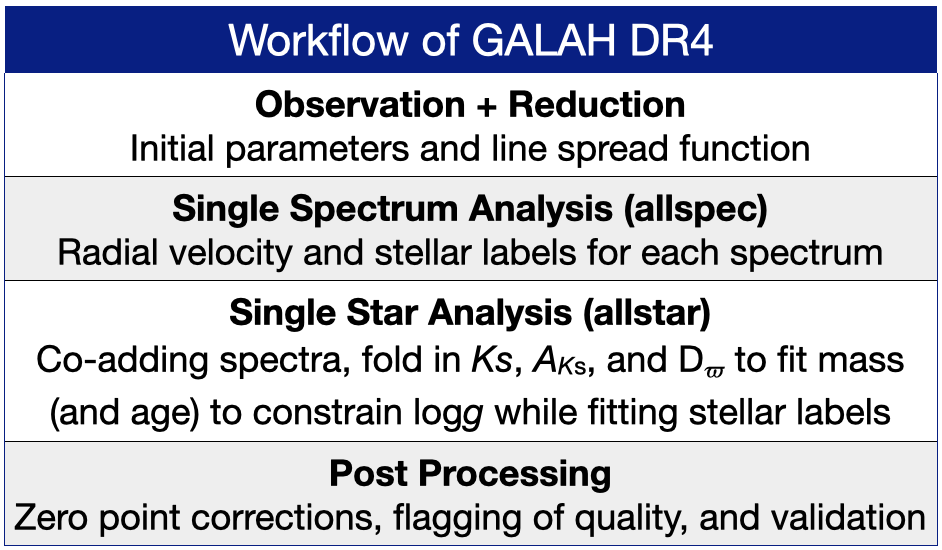
\includegraphics[width=\textwidth]{figures/workflow_galah_dr4.png}
 \caption{\textbf{Workflow of GALAH DR4.}}
 \label{fig:workflow_galah_dr4}
\end{figure}

%%%%%%%%%%%%%%%%%%%%%%%%%%%%%%%%%%%%%%%%%%%%%%%%%%%%%%%%%%%%%%%%%%%%%%%%%
\section{DATA}
\label{sec:data}
%%%%%%%%%%%%%%%%%%%%%%%%%%%%%%%%%%%%%%%%%%%%%%%%%%%%%%%%%%%%%%%%%%%%%%%%%

The GALAH Survey uses the 3.9-metre Anglo-Australian Telescope at Siding Spring Observatory on Gamilaraay Country and its Two-Degree Field positioning system (2dF) top end \citep{Lewis2002}. 2dF magnetically places up to 400 fibre entrances on one of two metal field plates, which can be tumbled to allow observing of one set of fibres while configuring the other. Light is delivered through the fibres to the High Efficiency and Resolution Multi-Element Spectrograph (HERMES) spectrograph \citep{Barden2010, Brzeski2011, Heijmans2012, Farrell2014, Sheinis2015} and dispersed into four non-contiguous wavelength bands in the optical that cover $\sim 1000\,\text{\AA}$ in the range of $4713-4903$ (blue CCD or CCD1), $5648-5873$ (green / CCD2), $6478-6737$ (red / CCD3), and $7585-7887\,\text{\AA}$ (infrared IR / CCD4). The data used in this data release is primarily based on observations of stars with said setup, but also makes use of auxiliary photometric and astrometric information for the stars where available.

In this Section, we describe which stars we have targeted as part of configured fields \citep{Miszalski2006} and observed (Sec.~\ref{sec:target_selection_observations}) with the 2dF-HERMES setup, including the first description of the second phase of GALAH observations (GALAH Phase 2) with a sharper focus on main-sequence turnoff stars to estimate more precise ages. In Sec.~\ref{sec:spectroscopic_data_from_galah_observations}, we briefly summarise the properties of the spectroscopic data and how they were reduced to one-dimensional spectra. We also point out major changes in the observations and reductions with respect to the previous (third) data release \citep{Buder2021}. We further elaborate on the auxiliary information that was used for the analysis in Sec.~\ref{sec:non-spec_data}.

\begin{figure*}[ht]
 \centering
 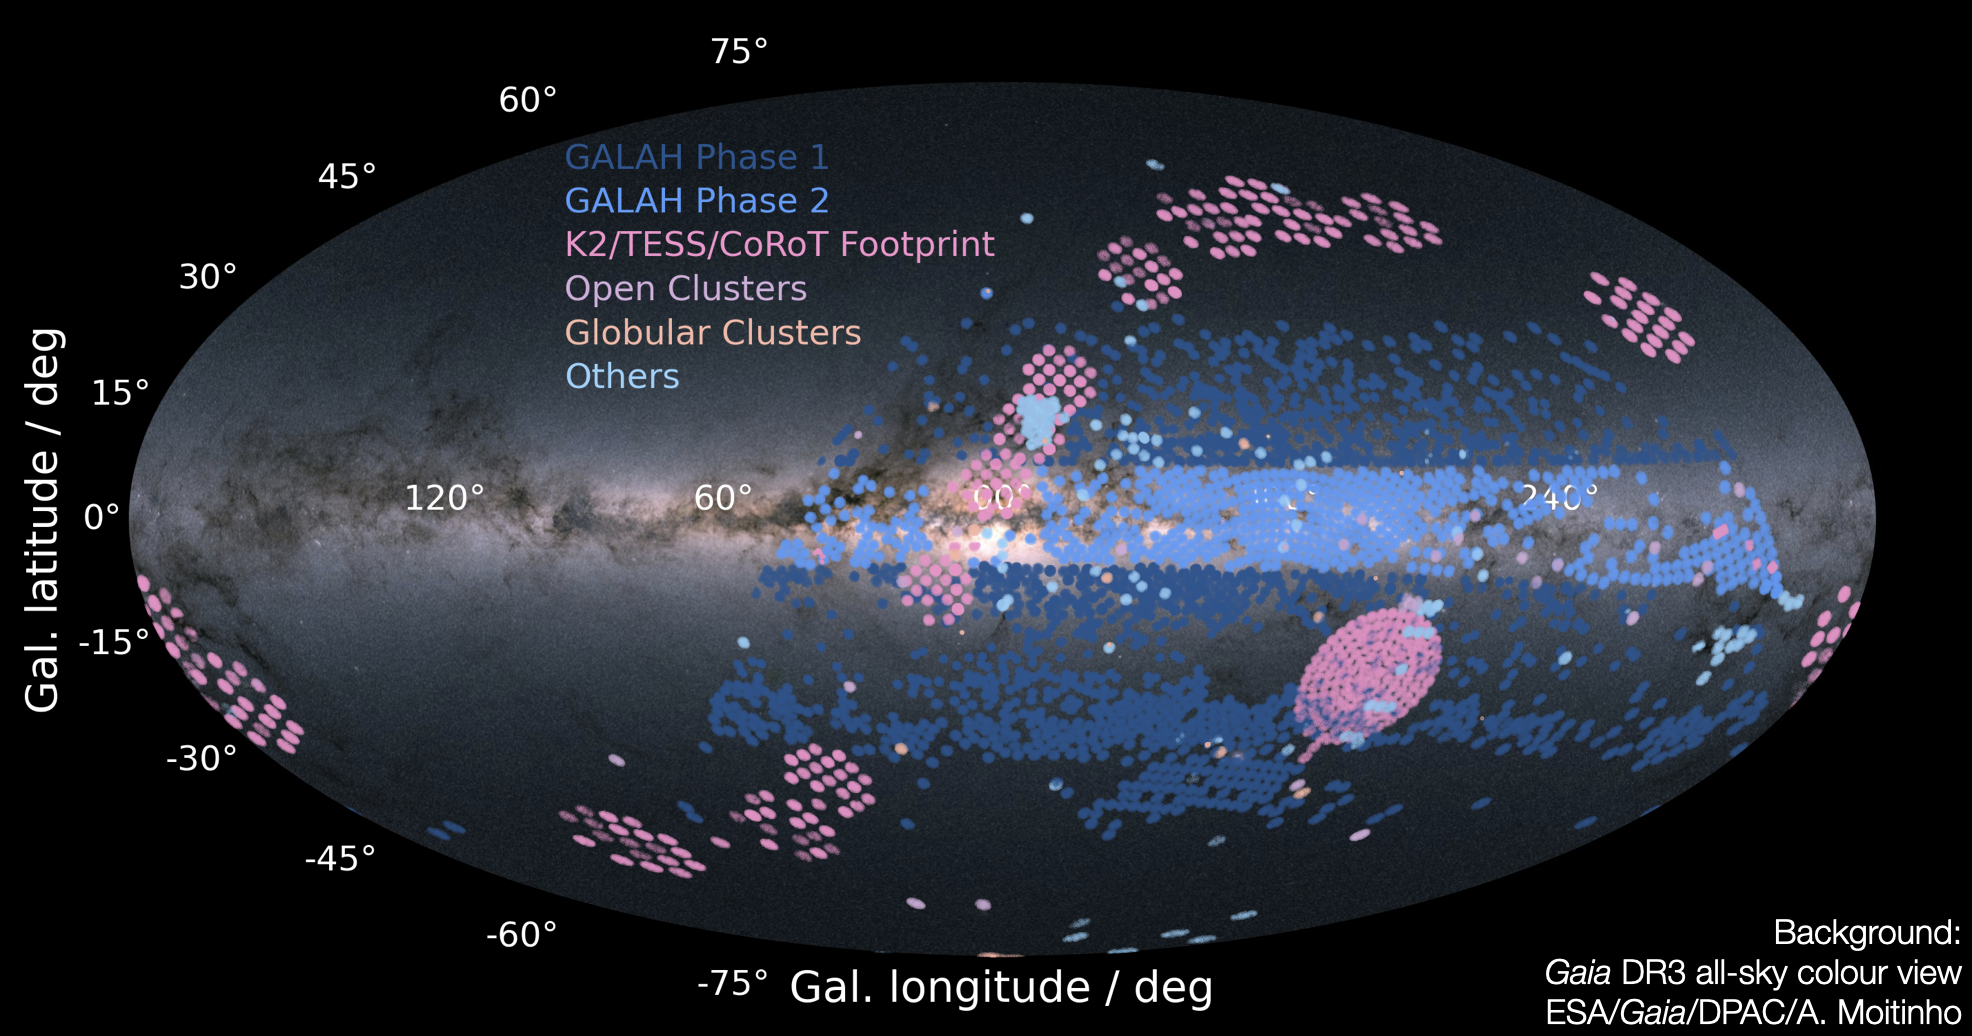
\includegraphics[width=\textwidth]{figures/galah_dr4_skymap_gaiadr3.png}
 \caption{\textbf{Overview of the distribution of stars included in this fourth GALAH data release in Galactic coordinates with the centre of the Galaxy at the origin and the \Gaia DR3 all-sky colour view \citep{GaiaDR3} as background.}
Shown are the targets of GALAH Phase 1 (dark blue) and Phase 2 (medium blue), the targets of the K2-HERMES follow-up along the ecliptic and TESS-HERMES in the TESS Southern Continuous Viewing Zone as well as CoRoT fields (pink). Both open and globular cluster points are shown in purple and orange, respectively. All other targets are shown in in light blue across the sky.
}
 \label{fig:galah_dr4_skymap_gaiadr3}
\end{figure*}

%%%%%%%%%%%%%%%%%%%%%%%%%%%%%%%%%%%%%%%%%%%%%%%%%%%%%%%%%%%%%%%%%%%%%%%%%
\subsection{Target selection and observational setup} \label{sec:target_selection_observations}
%%%%%%%%%%%%%%%%%%%%%%%%%%%%%%%%%%%%%%%%%%%%%%%%%%%%%%%%%%%%%%%%%%%%%%%%%

GALAH DR4 is a combination of the main GALAH survey and additional projects to observe asteroseismic targets from the K2 \citep{Sharma2019} and TESS missions \citep{Sharma2018}, as well as hand-picked and random observations as part of other programs. Additional proposals with 2dF-HERMES have contributed targeted observations of globular cluster members (PI M. McKenzie and PI M. Howell), open clusters (PI G. De Silva and PI J. Kos), young stellar associations (PI J. Kos), and halo stars (PI S. Buder) in addition to their observation through the main surveys. The column \texttt{survey\_name} in our catalogues denotes this origin. An all-sky view of GALAH DR4 is shown in Fig.~\ref{fig:galah_dr4_skymap_gaiadr3}.

\subsubsection{Target selection for GALAH Phase 1 and 2}

For GALAH Phase 1, we used the 2MASS photometric survey \citep{Skrutskie2006} with its $J$ and $Ks$ filters as a parent sample from which we selected stars within estimated visual magnitudes
\begin{equation}
V_\mathrm{JK} = K_S+2(J-K_S+0.14)+0.382e^{((J-K_S-0.2)/0.5)}.
\end{equation}

For GALAH Phase 1, a tiling pattern (with unique \texttt{field\_id} entries) with $2\,\mathrm{deg}$ fields of view below declination $\delta < +10\,\mathrm{deg}$ were created for regions with Galactic latitude $\vert b \vert > 10\,\mathrm{deg}$ to avoid crowding and strong extinction. For each tile, a selection of 400 stars within magnitudes $9 < V_\mathrm{JK} < 12$ for a bright magnitude cut and $12 < V_\mathrm{JK} < 14$ for the nominal magnitude cut is randomly selected from the complete parent sample of 2MASS. This typically selects 2/3 main sequence and turnoff stars and 1/3 evolved stars.

For GALAH Phase 2, a stronger focus on turn-off stars was implemented with the photometric and astrometric information of \Gaia data release 2 as a parent sample. For each field, we therefore first allocate fibres to stars with absolute magnitude between $2 < M_G < 4$, where
\begin{equation}
M_G = \texttt{phot\_g\_mean\_mag} + 5 \cdot \log_{10} \left( \frac{\texttt{parallax}}{100\,\mathrm{mas}} \right)
\end{equation}
with $G$ magnitude and parallax measurements from \Gaia DR2 \citep{Brown2018, Evans2018, Lindegren2018}. Remaining fibres are again filled with targets as done in Phase 1.

\subsubsection{Observational setup}

\begin{figure*}[ht]
 \centering
 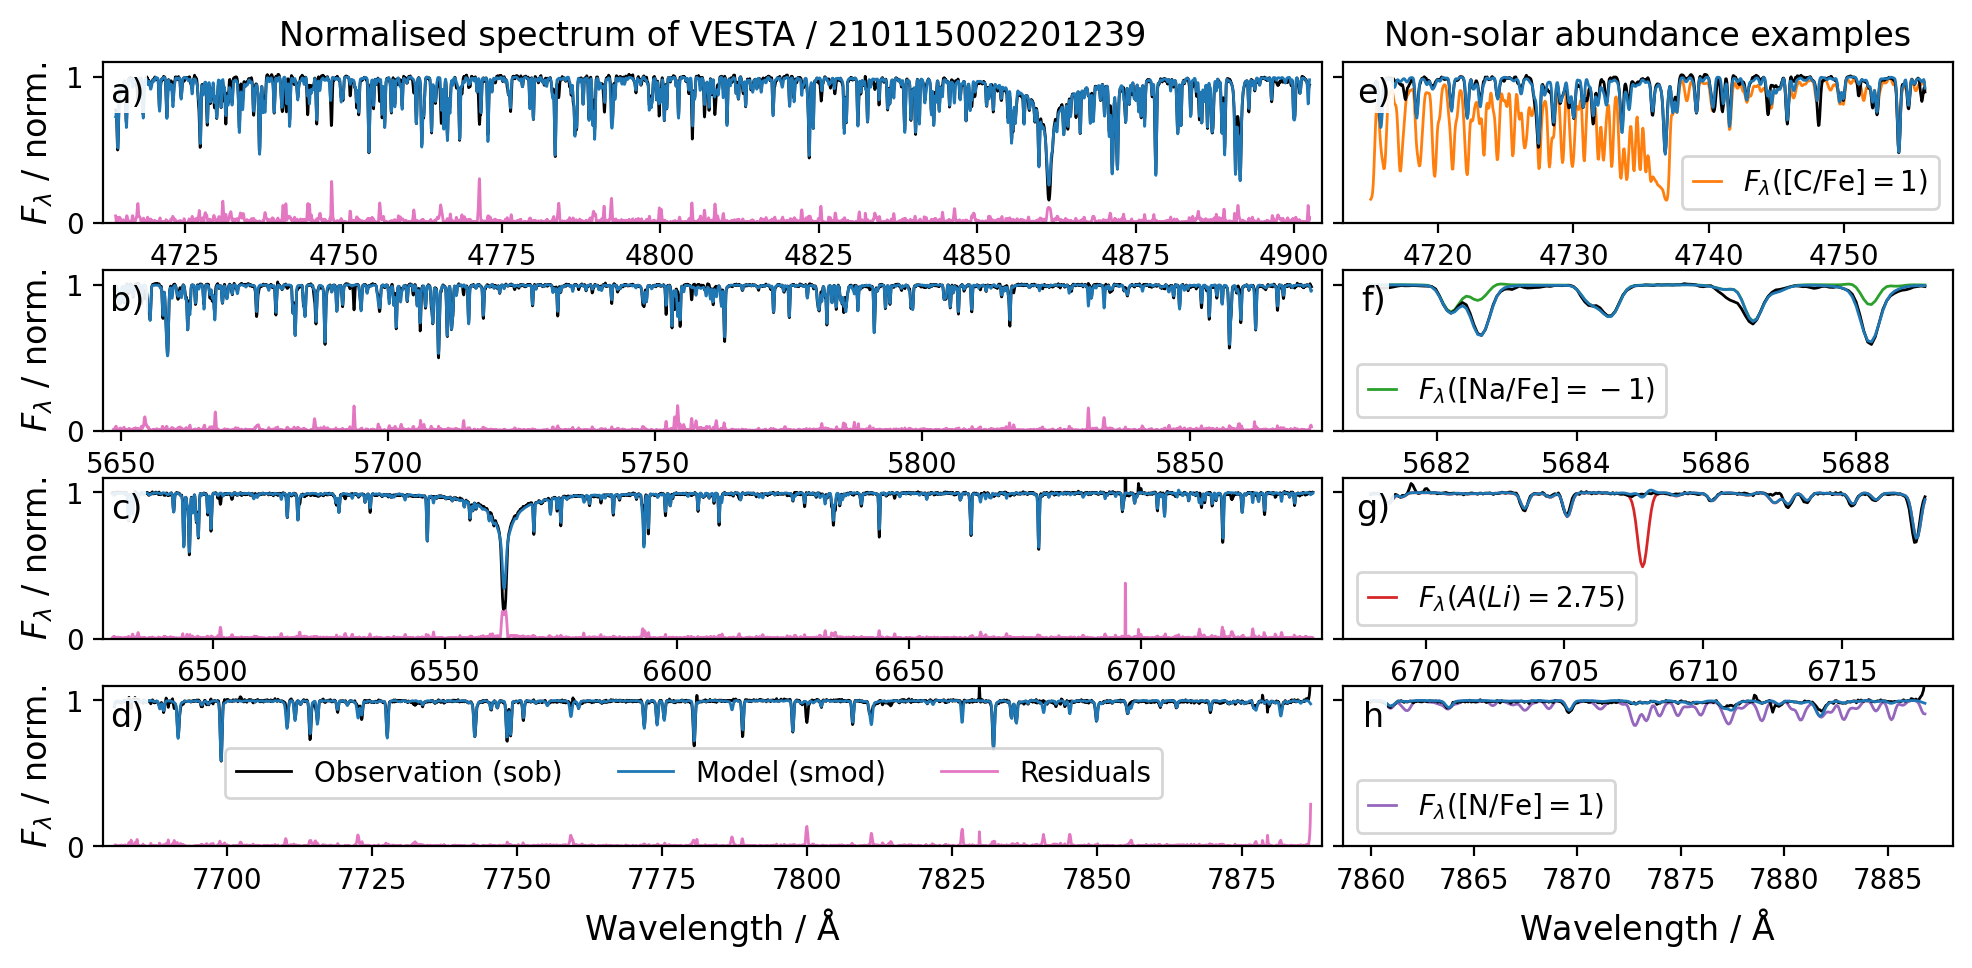
\includegraphics[width=\textwidth]{figures/210115002201239_abundance_examples.png}
 \caption{\textbf{Comparison of normalised observed (black) and synthetic spectra (blue) of the asteroid 4 Vesta with solar composition as well as examples of synthetic spectra with non-solar abundances.}
 \textbf{Panels a-d)} show the observed and best-fit synthetic spectrum as well as their absolute residual (pink) for the four wavelength channels of the HERMES spectrograph.
 \textbf{Panel e)} shows the beginning of the blue CCD 1 (left-most part of panel a) with an additional synthetic spectrum with ten times higher [C/Fe] in orange, for which the $\mathrm{C}_2$  Swan bands are prominent.
 \textbf{Panel f)} shows the beginning of the green CCD 2 (left-most part of panel b) and exemplifies with a synthetic spectrum in green that also has a ten times lower [Na/Fe] abundance (for example, in accreted stars) can still be reliably detected. 
 \textbf{Panel g)} shows the end of the red CCD 3 with a synthetic spectrum of primordial Li abundance of $\mathrm{A(Li)} = 2.75$ in red. While this abundance could be detected, the line for the Solar value $\mathrm{A(Li)} = 1.05$ is barely detectable.
 \textbf{Panel h)} shows the end of the infrared CCD 4, which would show strong molecular absorption features of the CN molecule for $\mathrm{[N/Fe]} = +1$ (purple).
 }
 \label{fig:210115002201239_abundance_examples}
\end{figure*}

We list the observations under various sub-programs in Table~\ref{tab:field_ids}. Except for 2\,935 spectroscopic observations with the high-resolution mode of HERMES ($R \sim 42\,000$) on 7, 8, 10, 11 and 12 February 2014, all observations were made in the low-resolution mode ($R \sim 28\,000$) with different total exposure times chosen for different programs, but typically between 60 and 90 minutes. Under sufficient conditions (no clouds and seeing below $2\,\mathrm{arcsec}$), GALAH Phase 1 and TESS-HERMES observed $3 \times 6$ minutes for bright targets ($9 < V_\mathrm{JK} < 12$) and $3 \times 20$ minutes for the majority of targets ($12 < V_\mathrm{JK} < 14$).


\begin{table}
\centering
 \caption{\textbf{Overview of stars observed for the programs included in this data release.} Numbers of open and globular cluster observations were estimated after observations as described in Sec.~\ref{sec:oc_gc}. We have observed 30 globular clusters (23 with $\geq$ 5 stars) and 361 open clusters (109 with $\geq$ 5 stars).}
\label{tab:field_ids}
\begin{tabular}{crcr}
\hline \hline
Program & No. Stars & Program & No. Stars \\
\hline
galah\_bright & 67\,680 & 
k2\_hermes & 117\,736\\
galah\_main & 434\,901 & 
tess\_hermes & 37\,129\\
galah\_faint & 33\,907 & 
globular clusters & 2\,509\\ % matched with Vasiliev and Baumgardt
galah\_phase2 & 172\,494 & 
open clusters & 3\,706\\ % matched with Cantat-Gaudin members
commissioning & 2\,625 & 
other & 44\,901\\
  \hline
 \end{tabular}
\end{table}

\begin{table}
    \centering
    \caption{Data product 1: FITS files of reduced spectra.}
    \label{tab:reduction_fits}
    \begin{tabular}{cc}
    \hline \hline
    FITS Ext. & Description \\
    \hline
    Ext. 0 & Un-normalised signal~/~counts \\
    Ext. 1 & Normalised signal (by reduction pipeline) \\
    Ext. 2 & Relative uncertainty of signal \\
    Ext. 3 & Subtracted sky signal~/~counts \\
    Ext. 4 & Applied telluric correction \\
    Ext. 5 & Scattered light~/~counts \\
    Ext. 6 & Cross-talk \\
    Ext. 7 & Resolution profile~/~FWHM \\
    \hline
    \end{tabular}
\end{table}

GALAH Phase 2 extended these times to $3 \times 10$ and $3 \times 30$ minutes, respectively, and included repeat observations of GALAH Phase 1 main targets with another $3 \times 15$ minutes. K2-HERMES observations targeted stars with $13 < V_\mathrm{JK} < 15$ or even $13 < V_\mathrm{JK} < 15.8$ to complement the K2 Galactic Archaeology Program \citep{Stello2015}. These fields were observed for 2 hours, similar to most globular and open cluster stars. Worse seeing conditions or thin clouds triggered between one ($2 < \mathrm{seeing} < 2.5\,\mathrm{arcsec}$) and 3 ($2.5 < \mathrm{seeing} < 3\,\mathrm{arcsec}$) additional exposures. In addition to the science frames, quartz fibre flat and ThXe arc lamp observations were taken directly before or after each set of science exposures, and bias frames were taken at the beginning or end of each observing night.

%%%%%%%%%%%%%%%%%%%%%%%%%%%%%%%%%%%%%%%%%%%%%%%%%%%%%%%%%%%%%%%%%%%%%%%%%
\subsection{Spectroscopic data from GALAH observations}
\label{sec:spectroscopic_data_from_galah_observations}
%%%%%%%%%%%%%%%%%%%%%%%%%%%%%%%%%%%%%%%%%%%%%%%%%%%%%%%%%%%%%%%%%%%%%%%%%

Since the commissioning of the HERMES spectrograph in late 2013 until 6 August 2023, the GALAH collaboration and its partners have observed and successfully reduced \allspecnumber spectra of \allstarnumber stars. Each single observation is given a unique \texttt{sobject\_} YYMMDDRRR01FFF that is based on its year (YY), month (MM), and day (DD) of observations, its exposure run number (RRRR), and the used fibre (FFF). A reduced example spectrum of the asteroid 4 Vesta (observed on 15 Januar 2014 during run 22 through fibre 239 with \texttt{sobject\_id} 210115002201239) is shown in Fig.~\ref{fig:210115002201239_abundance_examples} and used as a reference for a Solar spectrum. The reduction process to create FITS files of reduced spectra from two-dimensional images of the cameras employs an updated and publicly available \href{https://github.com/sheliak/galah_reduction/blob/master/extract6.0.py}{version 6} of the already well-tested reduction pipeline \citep{Kos2017}. The file extensions are listed in Tab.~\ref{tab:reduction_fits} and created as follows.

Science frames are corrected by removing the bias, dividing out the different gain of the two readout amplifiers per CCD, flagging bad pixels, and dividing by master flatfield frames, as well as removing cosmic rays and scattered light. Subsequently, apertures for each fibre trace are identified and used to extract the individual spectra. 

Wavelength calibrations are performed via Chebyshev polynomial functions based on the ThXe arc frames and the spectra are interpolated onto a linearly increasing wavelength grid. The starting wavelength \texttt{CRVAL1} and dispersion \texttt{CDELT1} are saved in the headers of each FITS file.

Finally, sky lines are subtracted and telluric features removed, before a barycentric correction is applied to create the `reduced' spectra that are saved in extension~1 of the reduction pipeline FITS files and used for the subsequent analysis. 

Fractional noise/uncertainties are saved in extension~2 and calculated from the square root of the sum of squared flux, sky features (extension~3), scattered light (extension~5), and crosstalk (extension~6) measurements as well as the squared readout noise.

The wavelength dependent line spread functions (LSFs) are measured from the arc calibration frames for each spectrum and CCD by fitting modified Gaussian distributions with a boxiness parameter $b$ and full width half maximum \texttt{fwhm} for each wavelength point in the spectrum, that is
\begin{align}
    \exp \left(-0.693147 \cdot \vert 2 \cdot \textbf{\textit{x}}/\texttt{fwhm} \vert^\texttt{b}\right) \label{eq:lsf}
\end{align}
The array $\textbf{\textit{x}}$ then includes the pixels around each wavelength step that are used to apply the convolution from higher resolution to GALAH resolution spectra. The fitted values of \texttt{fwhm} are saved in extension~7 with $b$ saved in the headers.

The achieved Signal-to-Noise Ratio (SNR) of the individual exposures depends on the spectral types, reddening, and observational conditions. Especially the repeat observations of previous pointings have increased the SNR for co-added spectra with respect to GALAH DR3. This can be appreciated from Fig.~\ref{fig:snr_distribution}, where we plot the cumulative distribution function for all stars of GALAH DR3 (dashed lines) and GALAH DR4 (solid lines) for the different CCDs. 

\begin{figure}[ht]
    \centering
    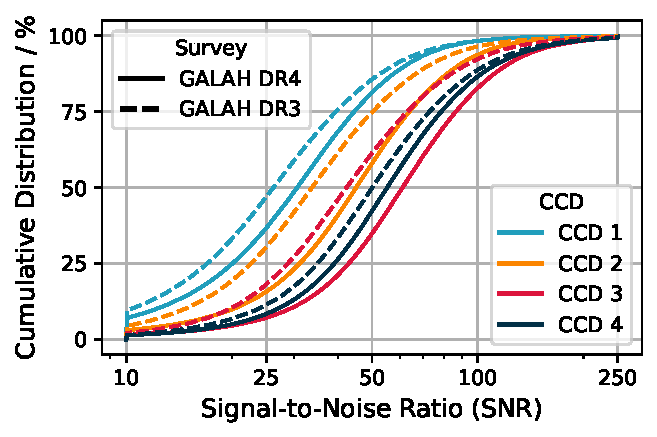
\includegraphics[width=\columnwidth]{figures/snr_distribution.pdf}
    \caption{Cumulative Distribution Function (CDF) of the logarithmic Signal-to-Noise Ratio (SNR) for the 4 CCDs of the HERMES spectrograph comparing GALAH DR4 (solid lines) and GALAH DR3 (dashed lines).}
    \label{fig:snr_distribution}
\end{figure}

%%%%%%%%%%%%%%%%%%%%%%%%%%%%%%%%%%%%%%%%%%%%%%%%%%%%%%%%%%%%%%%%%%%%%%%%%
\subsection{Auxiliary data from \Gaia, 2MASS, and literature} \label{sec:non-spec_data}
%%%%%%%%%%%%%%%%%%%%%%%%%%%%%%%%%%%%%%%%%%%%%%%%%%%%%%%%%%%%%%%%%%%%%%%%%

%SELECT
%galah.sobject_id,
%tmass.designation as tmass_id,
%tmass.ph_qual as tmass_ph_qual,
%tmass.ra as raj2000,
%tmass.dec as dej2000,
%tmass.j_m, tmass.j_msigcom,
%tmass.h_m, tmass.h_msigcom,
%tmass.ks_m, tmass.ks_msigcom,
%calj.r_med_geo,calj.r_lo_geo,calj.r_hi_geo,
%calj.r_med_photogeo,calj.r_lo_photogeo,calj.r_hi_photogeo,
%calj.flag as calj_flag,
%gaia.*
%FROM gaiadr3.gaia_source as gaia
%LEFT OUTER JOIN
%	external.gaiaedr3_distance as calj
%	ON calj.source_id = gaia.source_id
%LEFT OUTER JOIN
%	gaiadr3.tmass_psc_xsc_best_neighbour AS tmassxmatch
%	ON tmassxmatch.source_id = gaia.source_id
%LEFT OUTER JOIN
%	gaiadr3.tmass_psc_xsc_join AS tmass_join
%	ON tmass_join.clean_tmass_psc_xsc_oid = tmassxmatch.clean_tmass_psc_xsc_oid
%LEFT OUTER JOIN
%	gaiadr1.tmass_original_valid as tmass
%	ON tmass.designation = tmass_join.original_psc_source_id
%INNER JOIN
%	user_sbuder.dr6_0_230101_unique_ids as galah
%	ON galah.tmass_id = tmass.designation

To support our spectroscopic analysis, we make use of astrometric and photometric information from the \Gaia satellite \citep{Gaia-Collaboration2016} and 2MASS survey \citep{Skrutskie2006}, which is available for essentially all our targets. We further use the value-added catalogues, like distance estimates for field stars by \citep{BailerJones2021} as well as open and globular cluster membership probabilities from \citet{CantatGaudin2020} as well as \citet{Vasiliev2021} and \citet{Baumgardt2021}.

\subsubsection{\Gaia DR3}

We crossmatch our observations to the \Gaia DR3 catalogue \citep{Brown2021,GaiaDR3} using the 2MASS ID, via the nearest neighbour crossmatches provided as part of \Gaia DR3 \citep{Torra2021}. 
911\,754 (99.0\,\%) also have astrometric information \citep{Lindegren2021a} and 849\,867 (93.0\,\%) have radial velocity estimates \citep{Katz2023}. We apply the corrections to both photometric \citep{Riello2021} and astrometric \citep{Lindegren2021b} information. Where possible we prefer the photogeometric distances over the geometric distances from \citep{BailerJones2021}. Where neither are available, we further try to find parallaxes from \cite{vanLeeuwen2007}. The average parallax uncertainty of the GALAH stars is $\sigma_{\varpi} / \varpi = 1.6_{-0.9}^{+2.6}\,\mathrm{\%}$. Only $2.3\,\%$ of GALAH stars have no parallax measurements or parallax measurements beyond $20\%$ uncertainty, for which the priors adopted by \citep{BailerJones2021} start to dominate distance estimates.

\subsubsection{2MASS, WISE, and extinction}

In addition to the excellent infrared photometry for 99.9\,\% of our sources from the 2MASS survey \citep{Skrutskie2006}, 98.7\,\% of them have far-infrared measurements from the WISE mission \citep{Cutri2013}. We therefore can estimate the extinction in the $K_S$ band via the RJCE method \citep{Majewski2011} $A_{K_S}  = 0.917 \cdot \left( H - W2 - 0.08 \right)$ for most stars. We confirm this estimate by estimating the extinction in $K_S$ via the extrapolation of the color extinction of $B-V$, that is, $A_{K_S} \sim 0.36 \cdot E(B-V)$ \citep{Cardelli1989}. We revert to this value if it is less than half the value of the RJCE estimate, or if either of the H and W2 bands does not have an excellent quality flag `A'. For negative estimates by the RJCE method and very nearby stars ($<100\,\mathrm{pc}$) we null the value.

\subsubsection{Open and Globular Cluster members and distances} \label{sec:oc_gc}

We identify open cluster members using the membership catalogue from \citet{CantatGaudin2020} via crossmatch with the \Gaia \texttt{source\_id} and adjust their parallaxes and distance estimates to the average cluster values if the latter are more precise. We identify globular cluster members (with more than 70\% probability) via the membership catalogue from \citet{Vasiliev2021} by crossmatching with the \Gaia \texttt{source\_id}. We then adjust the parallaxes and distances for the member stars to the mean values listed by \citet{Baumgardt2021}.

%%%%%%%%%%%%%%%%%%%%%%%%%%%%%%%%%%%%%%%%%%%%%%%%%%%%%%%%%%%%%%%%%%%%%%%%%
\section{SYNTHETIC SPECTRA FOR 2DF-HERMES}
\label{sec:synthetic_spectra}
%%%%%%%%%%%%%%%%%%%%%%%%%%%%%%%%%%%%%%%%%%%%%%%%%%%%%%%%%%%%%%%%%%%%%%%%%

The aim of our spectroscopic analysis is to estimate the best set of stellar properties (labels) that influence a stellar spectrum by minimising the difference between observed stellar spectra and synthetic ones that were created with those best stellar labels. In our endeavour to push the limits even further, we are advancing our analysis to fit all 31 elemental abundances and stellar parameters across the full GALAH wavelength range simultaneously with the appropriate model spectrum.

To make this computationally feasible, we follow an idea reported by \citet{Rix2016} and create flexible models for smaller regions of the parameter space from only a limited number of \textit{ab initio} models \citep[see also][]{Ting2016b}. Our \textit{ab initio} models are calculated with Spectroscopy Made Easy \citep[\sme][]{Valenti1996,Piskunov2017} for the whole wavelength range and all visible atomic and molecular lines for random selections of elemental abundances and stellar parameters within the range of \marcs atmospheres \citep{Gustafsson2008} at much higher resolution and sampling than our HERMES spectra. We then select subsets of these spectra within a restricted space of the three main spectroscopic parameters \Teff, \logg, and \feh. This idea is comparable to selecting Solar or stellar twin spectra when analysing the Sun \citep[see e.g.]{Nissen2015} or differential abundance analysis of globular cluster stars \citep[e.g.]{Yong2013, Monty2023}. As they reduce the impact of several systematic issues of line data and atmospheric effect, these approaches have been highly successful \citep{Nissen2018}. For each subset, we train a neural network that correlates stellar flux and labels (stellar parameters and abundances) similar to \textit{The Payne} \citep{Ting2019}. With these models, we can then create model spectra with all lines over the whole wavelength range for any combination of element abundances within this restricted parameter space within less than a second (as compared to minutes or hours for physics-driven syntheses). 

Another reason to create smaller training sets rather than a "one-fit-all" approach was the limited flexibility of both quadratic and non-linear interpolation routines within computationally reasonable model sizes and ability to test the model accuracy over the full parameter space. Surveys like GALAH, RAVE and APOGEE aim to fit basically all types of spectra at once. This means we demand one model to predict Sun-like stars, red clump stars, metal-poor stars with almost no absorption features, cool evolved stars with strong molecular features, and hot stars with shallow and broad lines - all at once and for up to 31 elemental abundances. As one can imagine, this is an impossible task and has led to numerous systematic trends in catalogues for the most extreme cases that use such model interpolations \citep{Casey2016,Buder2018,Ting2019}. In this data release, we therefore purposefully limit the spectral complexity by creating smaller models. The hot star model therefore does not need to also predict the strong molecular absorption features of a cool star. We discuss the possible caveats and disadvantages of this approach and our particular implementation in Sec.~\ref{sec:caveats}.

In this section, we lay out how we create smaller bins in the parameter space from which we sample a training set (Sec.~\ref{sec:higher_resolution_synthetic_spectra}) rather than using one training set for all stars. We describe how we create the parent sample of high-resolution synthetic stellar spectra (Sec.~\ref{sec:higher_resolution_synthetic_spectra}) and train neural networks to quickly predict/interpolate new synthetic spectra (Sec.~\ref{sec:interpolating_synthetic_spectra_with_neural_networks}).

%%%%%%%%%%%%%%%%%%%%%%%%%%%%%%%%%%%%%%%%%%%%%%%%%%%%%%%%%%%%%%%%%%%%%%%%%
\subsection{Stellar twin training sets rather than one-fits-all}
\label{sec:spectrum_grid}
%%%%%%%%%%%%%%%%%%%%%%%%%%%%%%%%%%%%%%%%%%%%%%%%%%%%%%%%%%%%%%%%%%%%%%%%%

\begin{figure}[ht]
 \centering
 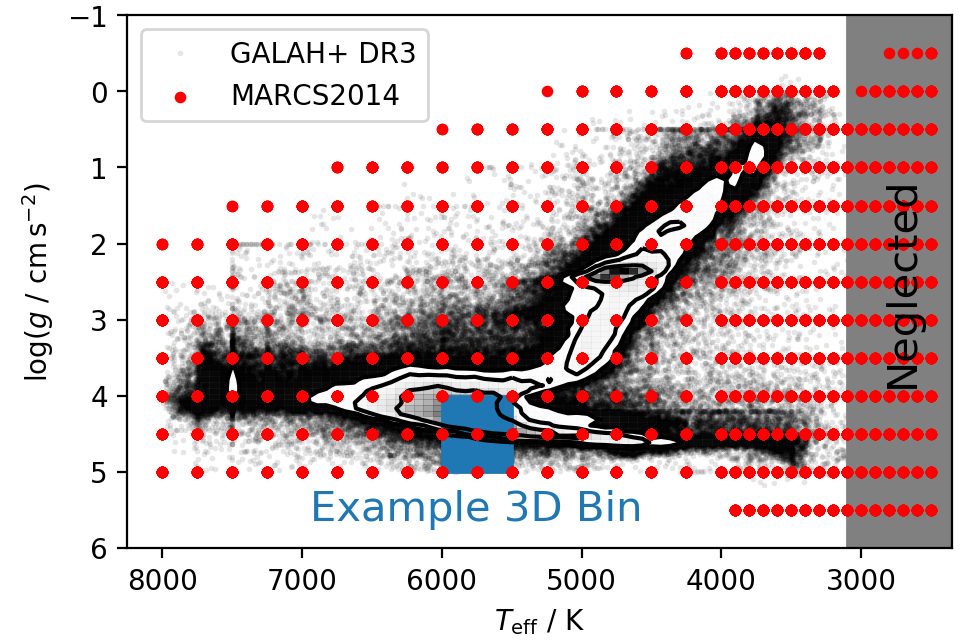
\includegraphics[width=\textwidth]{figures/teff_logg_grid_coverage.png}
 \caption{\textbf{Coverage in \Teff and \logg of the MARCS2014 grid (red) and GALAH DR3 (black, including density countours).} Shown is also an example of one of the 3D bins used to create models with \TheCannon. MARCS grid points \Teff$ < 3100\K$ or \feh$<-3\dex$ are neglected throughout GALAH DR4.}
 \label{fig:teff_logg_grid_coverage}
\end{figure}

The base grid for our training set computation is the \marcs grid \citep{Gustafsson2008}, which is shown with red points in Fig.~\ref{fig:teff_logg_grid_coverage}. Following the aforementioned idea of restricting ourselves to stellar siblings, we create multiple 3-dimensional bins in \Teff, \logg, and \feh within $\pm 1$ grid points in \Teff (with either $\pm 250$ or $\pm 100\K$), \logg ($\pm 0.5\dex$), and \feh ($\pm 0.5$ or $\pm 0.25\dex $). An example box is shown for Solar siblings as a blue box in Fig.~\ref{fig:teff_logg_grid_coverage}, which is centred on $T_\text{eff} = 5750\pm250\K$, $\log g = 4.5\pm0.5\dex$ and $\mathrm{[Fe/H]} = 0.0\pm0.25\dex$.

Within these bins we sample 280\footnote{This number is chosen to match the 28 CPUs of our computing nodes.} synthetic spectra with no rotational broadening, which are later broadened with different rotational velocities \vsini to create between 1680 and 2240 training set spectra for each bin. For clarity, we explain the parameter and abundance sampling for an example 3D bin centred on $T_\text{eff} = 5750\pm250\K$, $\log g = 4.5\pm0.5\dex$ and $\mathrm{[Fe/H]} = 0.0\pm0.25\dex$ (see blue box in Fig.~\ref{fig:teff_logg_grid_coverage}).

\begin{figure*}[ht]
 \centering
 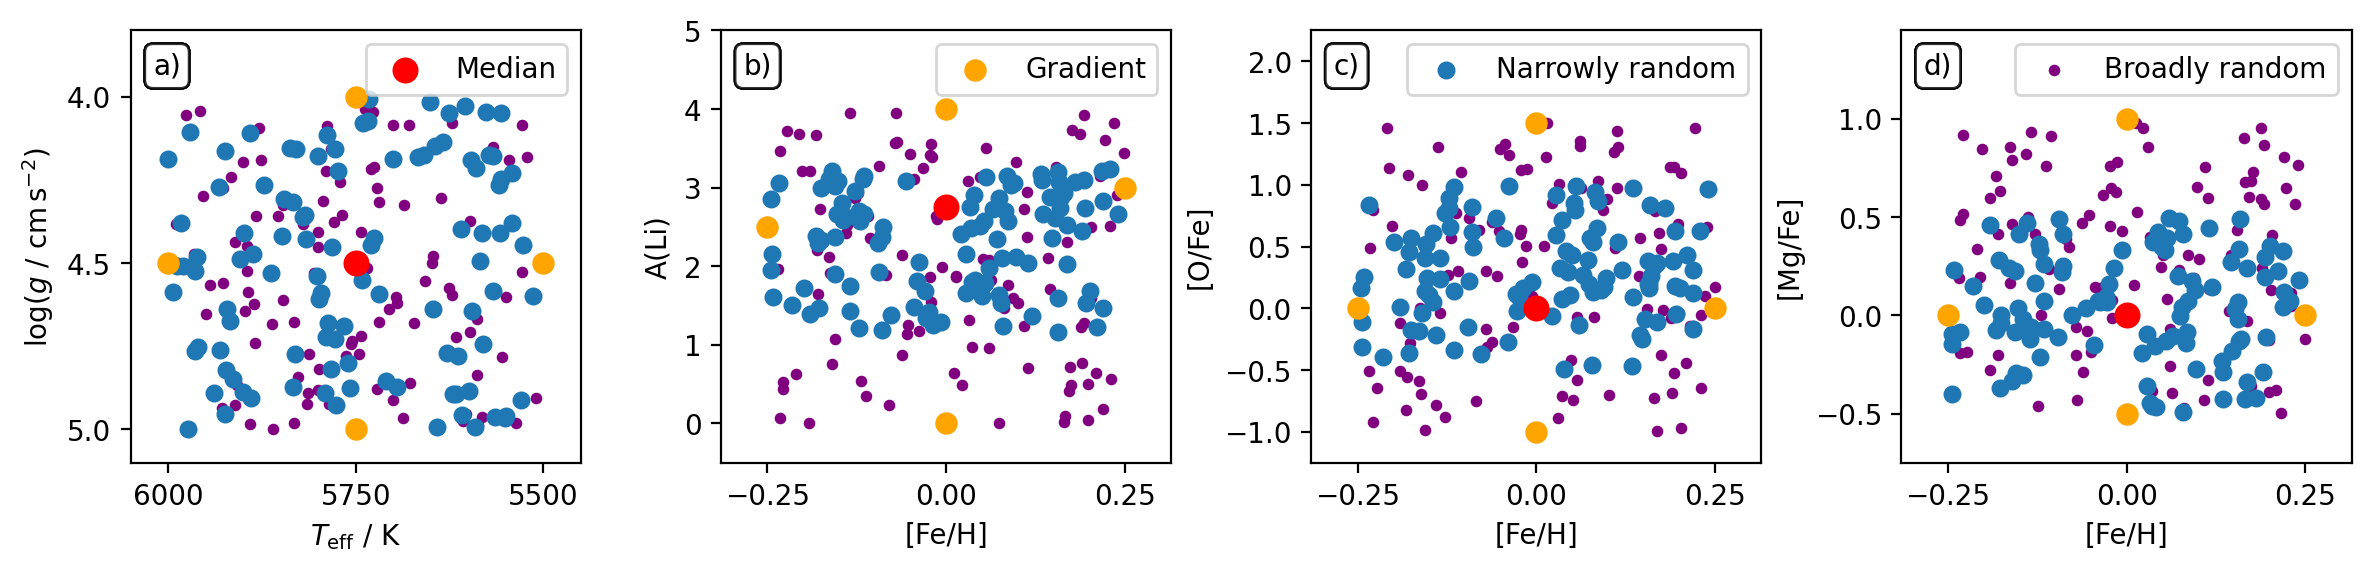
\includegraphics[width=\textwidth]{figures/example_3d_bin_sample.png}
 \caption{\textbf{Coverage of stellar parameters and abundances for one of the 3D bins.} Shown is the example of the Solar 3D bin ($T_\mathrm{eff}~/~\mathrm{K} = 5750$, $\log g~/~\mathrm{dex} = 4.5$, $\mathrm{[Fe/H]}~/~\mathrm{dex} = 0.0$). \textbf{Panel a):} \Teff and \logg, \textbf{Panel b):} [Fe/H] vs. A(Li), \textbf{Panel c):} [Fe/H] vs. [O/Fe], \textbf{Panel d):} [Fe/H] vs. [Mg/Fe]. While \Teff, \logg, and \feh are sampled randomly within the 3D bin, the abundances are sampled both narrowly (blue) and broadly (purple) within limits as described in the text. Red points indicate the median label values and orange points the adjusted label values to test the gradient change of spectra with individual labels.}
 \label{fig:example_3d_bin_sample}
\end{figure*}


\begin{table*}[ht]
\centering
 \caption{Example of boundaries for the uniform sampling of synthetic spectrum labels (stellar parameters and elemental abundances) for the 3-dimensional bin of Solar siblings \texttt{5750\_4.50\_0.00}.}
\label{tab:sampling_xfe}
\begin{tabular}{lclclc}
\hline \hline
Parameter & Sampling & Element & Sampling Narrow & Element & Sampling Broad \\
\hline
$T_\text{eff}~/~\K$ & 5500..5750..6000 & $\mathrm{A(Li)}$ & {1.05..2.75..3.26} & $\mathrm{A(Li)}$ & {0.00..4.00} \\
$\log g~/~\dex$ & 4.0..4.5..5.0 &  $\mathrm{C,~N,~O}$ & {-0.5..0.0..1.0} & $\mathrm{C,~N,~O}$ & {-1.0..1.5} \\
$\mathrm{[Fe/H]}~/~\dex$ & {-0.25..0.0..0.25} & $\mathrm{Y,~Ba,~La,~Ce,~Nd}$ & {-0.5..0.0..1.0} & $\mathrm{Y,~Ba,~La,~Ce,~Nd}$ & {-1.0..1.5} \\
$v_\text{mic}~/~\kms$ & {0.5,1.5,4.0}, but see Eq.~\ref{eq:vmic_initial} & $\mathrm{[X/Fe]~for~Mg,~Si,~Ti}$  &  {-0.5..0.0..0.5}& $\mathrm{[X/Fe]~for~Mg,~Si,~Ti}$ & {-0.5..1.0} \\
$v \sin i~/~\kms$ & 0.0\text{, but see Eq.~\ref{eq:vsini}} & $\mathrm{[X/Fe]~for~all~other~elements}$ & {-0.5..0.0..0.5} & $\mathrm{[X/Fe]~for~all~other~elements}$ & {-1.0..1.0}  \\
\hline \hline
\end{tabular}
\end{table*}

Stellar parameters (\Teff, \logg, \feh, \vmic) and elemental abundances [X/Fe] of all 30 elements are randomly sampled within reasonable limits (see examples in Tab.~\ref{tab:sampling_xfe}) and fed into \sme to create self-consistent synthetic spectra over the full HERMES wavelength range for \marcs atmospheres. 

\vmic values are sampled uniformly between the upper and lower limits of the empirical relation from GALAH DR3 \citep[Eqs.~4 and 5 from][]{Buder2021} and an adjusted version of the relation by \citet{DutraFerreira2016}. The latter has been adjusted for $T_\text{eff}^\prime = T_\text{eff} - 5500\,\mathrm{K}$ as well as $\log g^\prime = \log g - 4.0$ to return:
\begin{align} 
v_\text{mic} = \begin{array}{l}
1.198 + 3.16 \cdot 10^{-4} \cdot T_\text{eff}^\prime - 0.253 \cdot \log g^\prime \\ - 2.86\cdot 10^{-4} \cdot T_\text{eff}^\prime \cdot \log g^\prime + 0.165 \cdot (\log g^\prime)^2
\end{array} \label{eq:vmic_initial}
\end{align}

%%%%%%%%%%%%%%%%%%%%%%%%%%%%%%%%%%%%%%%%%%%%%%%%%%%%%%%%%%%%%%%%%%%%%%%%%
\subsection{Higher-resolution synthetic spectra with \sme}
\label{sec:higher_resolution_synthetic_spectra}
%%%%%%%%%%%%%%%%%%%%%%%%%%%%%%%%%%%%%%%%%%%%%%%%%%%%%%%%%%%%%%%%%%%%%%%%%

We create training sets from high-resolution stellar spectra for each smaller 3D bin region of the parameter space. We compute over-sampled synthetic intensity spectra at ten times higher resolution than the typical GALAH resolution with \sme for seven equal-area angles of a stellar surface (see Fig.~\ref{fig:sme_mu_output}).

\begin{figure*}[ht]
 \centering
 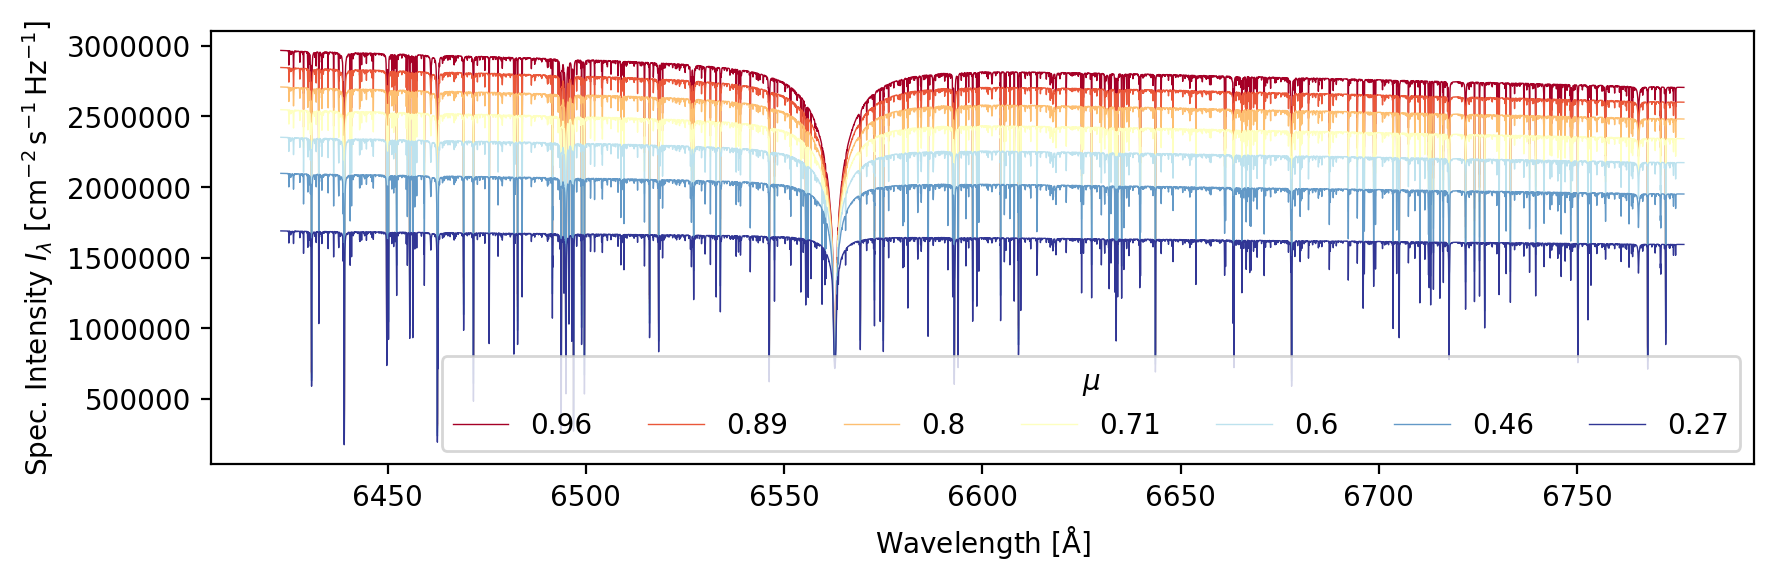
\includegraphics[width=\textwidth]{figures/solar_twin_specific_intensity.png}
 \caption{\textbf{Example output of \sme for a solar spectrum in HERMES CCD3 (around the Balmer $\mathrm{H}_\upalpha$ line).} Shown are the specific intensities (\texttt{sme.sint}) as a function of the viewing angle $\mu = \cos \theta$. }
 \label{fig:sme_mu_output}
\end{figure*}

For each spectrum, we first run a test on all available lines in the GALAH linelist. We use the same linelist as in GALAH DR3 \citep{Buder2021}. This linelist was adapted from the linelist by \citet{Heiter2021} and implements numerous updates to line data, such as updates or corrections of $\log gf$ values in the GALAH wavelength range. The test is used to restrict the myriad of possible molecular lines to the visible ones with \textsc{sme}.depth above 0.001, while keeping all atomic lines for the final synthesis.

Spectra are computed at a resolution of $R = 300,000$ on a fine wavelength grid with 60,819 pixels spread over the extended wavelengths $4675.1-4949.9$, $5624.1-5900.9$, $6424.1-6775.9$, and $7549.1-7925.9 \Angstroem$. We note that these extend significantly beyond the actual GALAH wavelength range.

We use 1D \marcs atmospheres from the \marcs grid \citep[][version 2014]{Gustafsson2008} and interpolate them for combinations of \Teff, \logg, and \feh. We use grids of non-LTE departure coefficients by \citet{Amarsi2020} for atomic lines of H, Li, C, N, O, Na, Mg, Al, Si, K, Ca, Mn, and Ba. For all except C, we use grids that include background scattering.

Our synthetic grid explicitly includes C and N abundances. C was previously included in the analysis of GALAH DR3, but limited to the atomic C line. The analysis thus neglected the molecular absorption features of $\mathrm{C_2}$ and CN at the beginning of CCD1 and end of CCD4, respectively. With the new self-consistent grid, we can include these features, as they hold valuable information for both C and N, as well as several other features through the molecular equilibrium in stars \citep[see e.g.][]{Ting2018}.

To be able to test that the flux-label correlations found by our polynomial interpolation are limited to reasonable wavelength ranges, we also calculate one spectrum that is exactly in the middle of the parameter range and additional spectra, where we increase the value of one label at a time (e.g. increase [O/Fe] by $1\dex$) to test the response in the synthetic spectrum.

To save computational costs, we compute synthetic spectra with no rotational or macroturbulence broadening ($v_\text{mac} = v\sin i = 0\kms$), but save the continuum flux (\texttt{sme.cmod}) and the specific intensities (\texttt{sme.sint}) as a function of the equal-area midpoints of each equal-area annulus $\mu$ (see Fig.~\ref{fig:sme_mu_output}). We then apply the broadening of spectra due to rotation (\vsini) with the flux integration code of the python-implementation \textsc{PySME} \citep{Wehrhahn2021} of \sme \citep{Piskunov2017}. Depending on the expected rotational velocities (increasing with temperature) we sample a range of
\begin{align} \label{eq:vsini}
    v \sin i~/~\kms \in \{ 1.5, 3, 6, 9, 12, 18, 24, 36\}.
\end{align}

Note that $v \sin i = 24 \kms$ is only included for bins with \Teff$\geq 5000\,\mathrm{K}$ and $v \sin i = 36 \kms$ for those with \Teff$\geq 6000\,\mathrm{K}$.

% The decision for these values was made based on the distribution of \vsini ($7.2_{-1.6}^{4.9}\kms$ with 90\% between 4.7 and $29.0\kms$) in GALAH+ DR3 \citep{Buder2021} and comparison with the grid values used by APOGEE DR16 \citep{Joensson2020}.

%%%%%%%%%%%%%%%%%%%%%%%%%%%%%%%%%%%%%%%%%%%%%%%%%%%%%%%%%%%%%%%%%%%%%%%%
\subsection{Interpolating synthetic spectra with neural networks} \label{sec:interpolating_synthetic_spectra_with_neural_networks}
%%%%%%%%%%%%%%%%%%%%%%%%%%%%%%%%%%%%%%%%%%%%%%%%%%%%%%%%%%%%%%%%%%%%%%%%

To allow a fast interpolation with new and different stellar labels, we use the method of training descriptive models to connect stellar fluxes at given pixels from a combination of stellar labels. This method is well established in stellar spectroscopy through the successful applications of quadratic models with \textit{The Cannon} \citep[see e.g.][]{Ness2015, Ness2016, Casey2016, Casey2017, Ho2017, Buder2018} as well as neural networks with \textit{The Payne} \citep[see e.g.][]{Ting2019, Xiang2019, Xiang2021}. Because of the needed flexibility\footnote{For a more detailed discussion on the advantages of neural networks for predicting spectra see \citet{Ting2019}.} to predict synthetic spectra with 36 stellar labels for a large parameter space, we are also choosing neural networks to interpolate between our synthetic spectra in this data release.

In this work, we utilize the neural network architecture and training algorithms from the spectrum interpolation framework of \textit{The Payne} \citep{Ting2019}. While we do not implement the full functionality of \textit{The Payne}, we specifically adopt its spectrum interpolation capabilities. Unlike the version originally published by \citet{Ting2019}, we use the architecture of the latest available version of \textit{The Payne}. This modified architecture connects stellar labels $\boldsymbol{\ell}$ with the flux $f$ at each wavelength pixel $\lambda$ via
\begin{equation}
f_\lambda = w \cdot \mathrm{lReLU} \bigg( \tilde{w}_\lambda^i \cdot \mathrm{lReLU}  \Big( w^k_{\lambda i} \ell_k + b_{\lambda i} \Big) + \tilde{b} \bigg) + \bar{f}_\lambda,
\label{eq:neural_network_function}
\end{equation}
which encapsulates the so-called layers of a neural network with $i = 300$ neurons and where we use the default leaky Rectified Linear Unit ($\mathrm{lReLU}$)
\begin{equation}
    \mathrm{lReLU} (x) =  \begin{cases}
        x \qquad &x \geq 0 \\
        0.01 x \qquad &x < 0.
    \end{cases}
\end{equation}

After optimizing the loss function for $10^4$ steps, we consider the network trained with an optimized combination of three sets of weights and biases within the minimum and maximum ranges of each label. We discuss the caveats of this particular neural network architecture and training setup in Section~\ref{sec:caveats}. The trained networks can then be used with new input labels to quickly create synthetic spectra for the label optimization.

%%%%%%%%%%%%%%%%%%%%%%%%%%%%%%%%%%%%%%%%%%%%%%%%%%%%%%%%%%%%%%%%%%%%%%%%%
\section{SINGLE SPECTRUM ANALYSIS (ALLSPEC)}
\label{sec:allspec_analysis}
%%%%%%%%%%%%%%%%%%%%%%%%%%%%%%%%%%%%%%%%%%%%%%%%%%%%%%%%%%%%%%%%%%%%%%%%%

As outlined in Sec.~\ref{sec:introduction}, the workflow of GALAH DR4 includes a first analysis step of all observed spectra without taking non-spectroscopic information for the optimization. This allows us to identify shifts in radial velocity between separate spectroscopic observations of the same star\footnote{While repeat observations were only done for quality assurance in GALAH Phase 1, a significant number of repeat observations was performed as part of Phase 2.} and a more accurate co-adding of spectra for the \texttt{allstar} analysis (see Sec.~\ref{sec:allstar_analysis}). Another motivation for this step is to get a first estimate of stellar labels without potentially biased photometric and astrometric information, for example for binary stars.

The optimization of stellar labels is thus aiming to minimise the absolute difference between synthetic and observed spectra, weighted by their uncertainty. Starting from a set of initial labels (Sec.~\ref{sec:initial_stellar_labels}), we create high-resolution synthetic spectra and convolve them to the resolution and wavelength grid of each observed spectrum. We remind ourselves that in GALAH DR3, we used a repeated combination of spectrum normalisation followed by stellar parameter optimization and a subsequent fit of individual elements with fixed stellar parameters. In the analysis of GALAH DR4, we perform an on-the-fly re-normalisation of the observed spectrum for every change of the simultaneously fitted stellar parameters and elemental abundances. This allows a more accurate comparison of synthetic and observed spectra (Sec.~\ref{sec:comparison_synthetic_spectra_to_observations}) and thus a more accurate stellar label optimization (see Sec.~\ref{sec:stellar_label_optimization}).

%%%%%%%%%%%%%%%%%%%%%%%%%%%%%%%%%%%%%%%%%%%%%%%%%%%%%%%%%%%%%%%%%%%%%%%%%
\subsection{Initial stellar labels}
\label{sec:initial_stellar_labels}
%%%%%%%%%%%%%%%%%%%%%%%%%%%%%%%%%%%%%%%%%%%%%%%%%%%%%%%%%%%%%%%%%%%%%%%%%

% https://github.com/svenbuder/GALAH_DR4/blob/main/spectrum_analysis/galah_dr4_initial_parameters.ipynb

Initial values of all stellar labels are needed for creating a first synthetic spectrum. For \vrad, \Teff, \logg, and \vsini we use a combination of sources. Where possible, we use the previous estimates from GALAH DR3 \citep{Buder2021}, and otherwise use estimates from the GALAH DR4 reduction pipeline (Sec.~\ref{sec:spectroscopic_data_from_galah_observations}). Because of the limited accuracy of the latter for cool stars with $T_\text{eff} < 4000\,\mathrm{K}$ as well as the hottest stars with $T_\text{eff} > 6500\,\mathrm{K}$, we perform a consistency check with photometric information from \Gaia DR3 \citep{Brown2021} and 2MASS \citep{Skrutskie2006}. For most of the aforementioned cool and hot stars, we therefore prefer the parameters from the \Gaia DR3 photometric pipeline GSP-Phot \citep{Andrae2022,Fouesneau2022} as initial values.

In selected cases, we further adjust the starting parameters toward reasonable limits, for example for hot stars which are likely to be young and close to Solar metallicity. Furthermore, we recalculate the initial \vmic based on Eq.~\ref{eq:vmic_initial} and limit rotational broadening values to $3 \leq v \sin i \leq 10\,\mathrm{km\,s^{-1}}$ for stars below $T_\text{eff} = 5500\,\mathrm{K}$ and $3 \leq v \sin i \leq 20\,\mathrm{km\,s^{-1}}$ for hotter stars. The explicit choices of starting values for \Teff, \logg, \feh, \vmic, and \vsini are described in our \href{https://github.com/svenbuder/GALAH_DR4/blob/main/spectrum_analysis/galah_dr4_initial_parameters.ipynb}{online repository} and are depicted in Fig.~\ref{fig:initial_parameters}.

Based on the value of \feh we apply an offset to the $\upalpha$-process elements O, Mg, Si, Ca, and Ti. The initial value is 0.4 for $\mathrm{[Fe/H]} < -1$, 0.0 for $\mathrm{[Fe/H]} > 0$, and $-0.4 \times \mathrm{[Fe/H]}$ for $-1 \leq \mathrm{[Fe/H]} \leq 0$. All other abundances are initialised at $\mathrm{[X/Fe]} = 0$.

%%%%%%%%%%%%%%%%%%%%%%%%%%%%%%%%%%%%%%%%%%%%%%%%%%%%%%%%%%%%%%%%%%%%%%%%%
\subsection{Comparison of synthetic spectra to observations}
\label{sec:comparison_synthetic_spectra_to_observations}
%%%%%%%%%%%%%%%%%%%%%%%%%%%%%%%%%%%%%%%%%%%%%%%%%%%%%%%%%%%%%%%%%%%%%%%%%

The major aim of our spectroscopic analysis is to predict the best set of stellar labels by minimising the uncertainty-weighted difference between observed and synthetic spectra. In this section, we describe several important steps to enable the pixel-level comparison of the higher resolution, oversampled synthetic spectra created with the neural networks from Sec.~\ref{sec:interpolating_synthetic_spectra_with_neural_networks} and the observational data at actually measured resolution and sampling (presented in Sec.~\ref{sec:spectroscopic_data_from_galah_observations}).

\subsubsection{Downgrading of synthetic spectra to observed resolution}

Because dedicated line-spread-function measurements are available for every spectrum (see Sec.~\ref{sec:spectroscopic_data_from_galah_observations}), we use this information to downgrade our synthetic spectrum to the measured resolution of each observation. We then interpolate the over-sampled synthetic spectrum onto the observed wavelength grid.

\subsubsection{On-the-fly re-normalisation of observed spectra}

Measurements of the GALAH flux and flux uncertainty are reported in counts by the reduction pipeline. To compare with our synthetic spectra, which are normalised to the continuum, we fit an outlier-robust polynomial function to the ratio of observed and synthetic spectrum and re-normalise our observed spectra and their uncertainties via this normalisation function.

This specific approach is similar to the internal routine of \sme \citep{Piskunov2017} and has the important advantage that no continuum points have to be defined. This is advantageous because we try to cover the full parameter range of FGKM stars for which positions of continuum points -- corresponding to 1 on a (pseudo-)continuum-normalised spectrum -- differ significantly or for which continuum points may not even be present (as is the case for M stars).

We make two additional adjustments to the reduced spectra, which come in the form of counts and uncertainty per wavelength, $f_\lambda$ and $\sigma_{f,\lambda}$.

\begin{figure*}[ht]
\centering
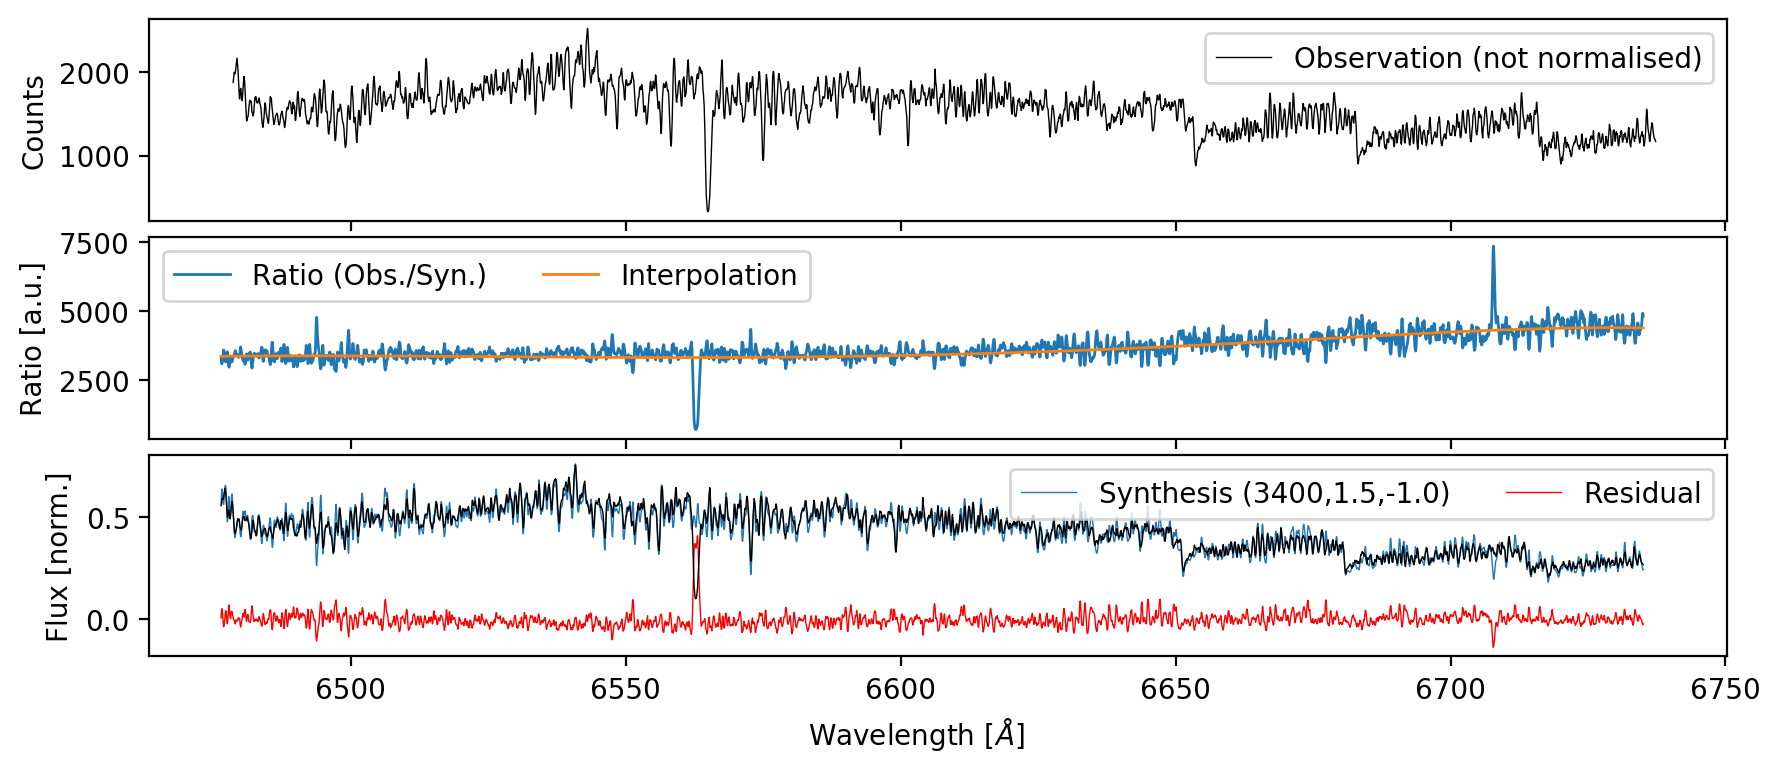
\includegraphics[width=\textwidth]{figures/Nuisance_example.png}
\caption{
\textbf{Example of normalisation for GALAH DR4 for a model spectrum ($T_\mathrm{eff} = 3400\,\mathrm{K}$, $\log g = 1.5$, $\mathrm{[Fe/H] = -1.0}$) that is selected during the label optimization.}
\textbf{Panel (a):} Observed spectrum (counts).
\textbf{Panel (b):} Ratio (blue) of observed spectrum and model spectrum as well as Chebyshev polynomial fit (orange).
\textbf{Panel (c):} Normalised observed spectrum (black) compared to the model spectrum (blue). Residuals (red) can then be used as input for the likelihood function.
}
\label{fig:ratio_normalisation}
\end{figure*}

As we compare the observation to model spectra, we do not have to restrict ourselves to an \textit{a priori} normalisation, but can take into account the residual information on the continuum in parts of the spectrum. For each model spectrum that we compare to, we therefore perform a normalisation by fitting a Chebyshev polynomial with outlier clipping to the ratio of model and observation (see Fig.~\ref{fig:ratio_normalisation}). This allows us to both overcome previous shortcomings of the synthetic analysis in GALAH+ DR3 \citep{Buder2021}, which had to be restricted to small wavelength segments and assumed a linear relation for those. Our new approach allows us to properly assess the structure of deep and steep molecular features that can dominate spectra of cool stars and carry significant information on \Teff as well as \vrad.

% \SB{Describe here the tests we do to make sure this actually provides a smooth transition between the different labels. Tests of the Cannon models show, that they can reproduce the spectra and their labels within for example $1\K$ \Teff, $0.01\dex$ \logg, and $0.01\dex$ \feh for the grid edges. But more thorough testing is needed.}
% \SB{Also keep in mind the issues found for \TheCannon with only 2 models applied to RAVE \citep{Casey2017}.}

%%%%%%%%%%%%%%%%%%%%%%%%%%%%%%%%%%%%%%%%%%%%%%%%%%%%%%%%%%%%%%%%%%%%%%%%%
\subsection{Stellar label optimization}
\label{sec:stellar_label_optimization}
%%%%%%%%%%%%%%%%%%%%%%%%%%%%%%%%%%%%%%%%%%%%%%%%%%%%%%%%%%%%%%%%%%%%%%%%%

In up to four major loops, we optimize the radial velocities and all other stellar labels and report a) their values, b) their co-variances, c) the best fit synthetic and re-normalised spectra along with d) their uncertainties and e) masks that indicate which pixels were used in the final optimization.

Starting from the initial values, a first synthetic spectrum is computed and compared with the observation in order to assess the initial radial velocity. This is done by applying the \textsc{scipy.signal.find\_peaks} algorithm on the normalised inverse residuals of non-shifted observed and synthetic spectra, when the latter is shifted by $v_\text{rad} = -1000..(2)..1000\kms$ (see Fig.~\ref{fig:181221003101356_single_fit_rv}a). If no peak is found, the initial \vrad value is used hereafter. If more than one peak is found (see Fig.~\ref{fig:181221003101356_single_fit_rv} with \Gaia DR3 agreeing with the systemic radial velocity), the two strongest peaks are reported. For the purpose of the single star analysis, a narrower search is conducted around the highest peak with a \vrad shift of $-20.00..(0.04)..20.00\kms$ around said peak by fitting a Gaussian function to the inverse of the residuals that were normalised with the smallest residual values (see Fig.~\ref{fig:181221003101356_single_fit_rv}c). The mean of this fit and its uncertainty are reported by the pipeline.

\begin{figure}[hbt]
\centering
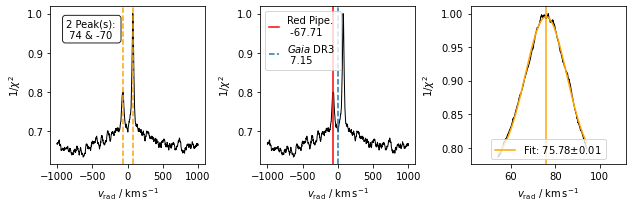
\includegraphics[width=\textwidth]{figures/181221003101356_single_fit_rv.png}
\caption{\textbf{Output of the radial velocity fitting step.} \textbf{Panel a)} shows the initial broad search on a \vrad array of $-1000..(2)..1000\kms$. In the case of 2MASS J06084657-7815235, two peaks (yellow, dashed) are visible for this double-lined spectroscopic binary. \textbf{Panel b)} shows the same plot, but overlaid with the GALAH DR4 reduction pipeline (red) and \Gaia DR3 (blue, dashed) estimates or \vrad. \textbf{Panel c)} shows the narrow window of $-20.00..(0.04)..20.00\kms$ around the highest peak and the Gaussian fit (yellow) to it.}
\label{fig:181221003101356_single_fit_rv}
\end{figure}

The centerpiece of our optimization is the \textsc{scipy.optimize} module's \textsc{curve\_fit} function \citep{scipy}, which we call with counts and uncertainties (our absolute sigmas) as input for a placeholder function that self-consistently re-normalises the observed spectrum. We estimate the labels via the least squares optimization within less than $10^4$ iterations and a desired relative error (\texttt{xtol}) below $10^{-4}$.

For each optimization loop, a new, best-fit 3D bin and neural network is identified via a grid search in the \TLF dimensions with \textsc{sklearn.cKDtree}. If the stellar labels that are being fitted have changed (for example if an element is deemed not detectable for the new 3D bin during the neural network training), the label and its value are either deleted or initialised with $\mathrm{[X/Fe]} = 0$.

While the optimization has not converged (the final parameters \TLF are not within the current 3D bin), the optimization is repeated, starting with the previous best-fit parameters as starting guesses.

We measured the time taken for the individual steps in the \textsc{curve\_fit} function's execution to be approximately $80\,\mathrm{ms}$. The total fitting process for stellar labels, including input/output overheads, was timed at $89_{-29}^{+77}\,\mathrm{s}$ for the \texttt{allspec} module, and $125_{-33}^{+81}\,\mathrm{s}$ for the more complex \texttt{allstar} module.

\begin{figure*}[ht]
\centering  
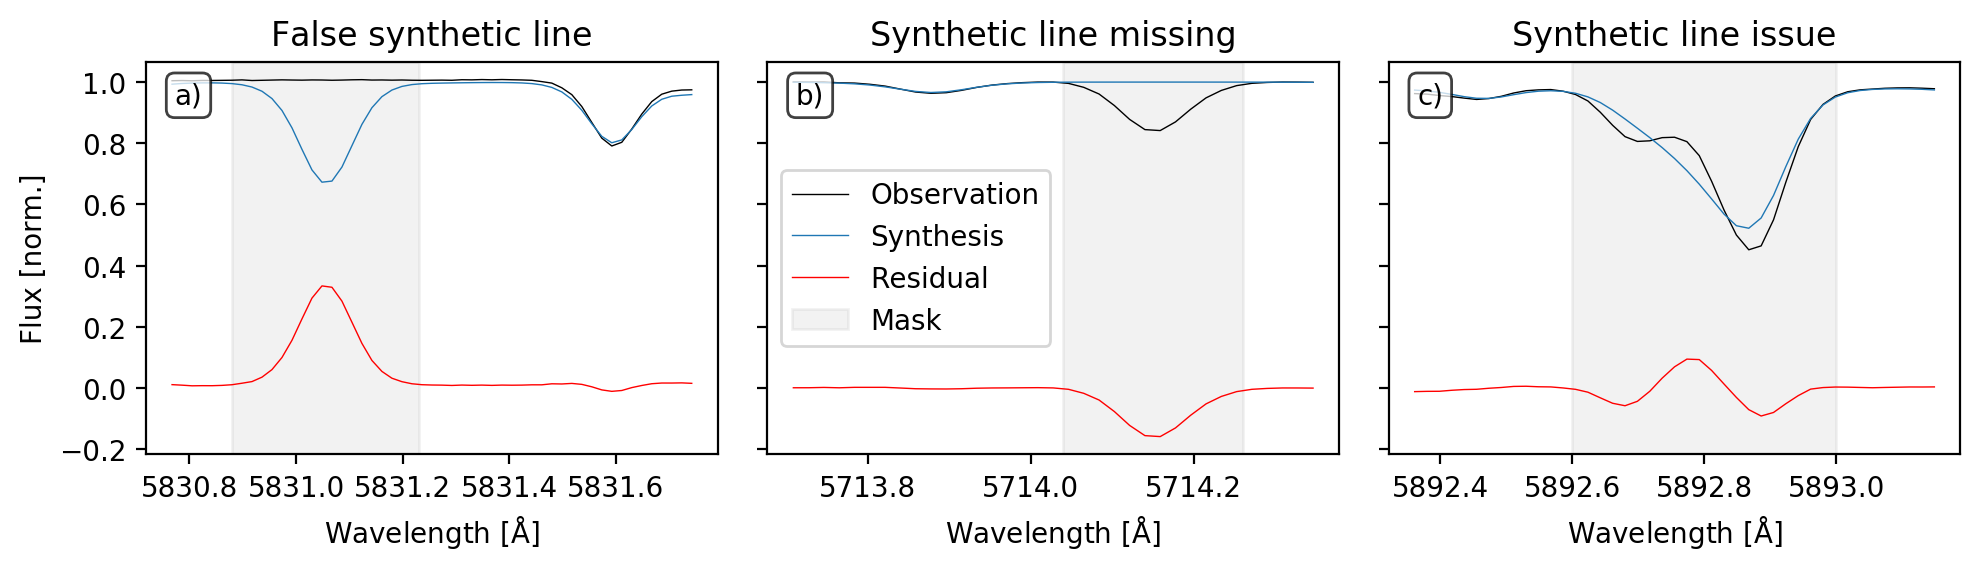
\includegraphics[width=\textwidth]{figures/example_masking_sun.png}
\caption{\textbf{Examples of masks applied to unreliable pixels for the spectrum fitting, which is done by the minimisation of residuals (red) between observation (black) and synthesis (blue).} \textbf{Panel a)} shows a strong synthetic line, where no line is observed in the data. \textbf{Panel b)} shows an observed line without any line being synthesised. \textbf{Panel c)} shows significant disagreement between the two observed lines and the synthesis.} \label{fig:example_masking_sun}
\end{figure*}

\subsubsection{Which stellar labels are optimized?} \label{sec:which_labels_are_optimized}

%% This paragraph is based on the combination of 
%% spectrum_interpolation/galah_dr4_grid_interpolation_recommend_labels.ipynb
%% and
%% spectrum_analysis/galah_dr4_spectrum_analysis_single.ipynb

As part of the synthetic grid computations, we have perturbed each label of stellar parameters and elemental abundances individually to our chosen maximum and minimum ranges (see Sec.~\ref{sec:spectrum_grid}). This allows us to also judge which stellar labels to fit for each given star. We choose to fit a stellar label if either of these two cases applies to said label for the GALAH wavelength range when neglecting the cores of the Balmer lines: Does the spectrum between minimum and maximum label value at any pixel change more than a certain threshold (0.07 of the normalised spectrum)? Does the spectrum between minimum and maximum label value change by more than 0.005 of the normalised spectrum for at least 25\% of the spectrum? While the first case is constructed for atomic lines, such as \ion{Li}{i} 6708\,\AA, the second case is addressing in particular molecular lines like the $\mathrm{C_2}$ and $\mathrm{CN}$ lines. For stars that are missing data from the infrared arm of HERMES (CCD4) we fix the abundances of N, O, L, and Rb to the scaled-Solar values.

Initial tests of the pipeline have revealed that in cases where the initial parameter estimates deviate significantly from the final values, several elemental abundance estimates were shifted towards their boundaries, leading to a masking of their elemental abundance lines by the masking module (Sec.~\ref{sec:masking_of_unreliable_wavelength_regions}) at the beginning of each optimization loop. To minimise this effect, we therefore shift the interim abundance values towards the narrow label boundaries. In practise, we limit the initial and interim abundances to 1.05..3.26 for A(Li), $\mathrm{[X/Fe]} = -0.5..1.0$ for C, N, O, Y, Ba, La, Ce, and Nd, and $\mathrm{[X/Fe]} = -0.5..0.5$ for all other elements before optimizing them again. For warm and hot stars ($T_\text{eff} > 6000\K$), this effect was seen to affect multiple abundances, such that we needed to implement a zeroing of all abundances except Li for stars above $6000\K$, which would on average be expected to be young and have a Solar-like composition.

\subsubsection{Masking of unreliable wavelength regions} \label{sec:masking_of_unreliable_wavelength_regions}

Not all pixels of the observed or synthetic spectra might prove useful for estimating reliable stellar labels. Observations can include bad pixels/patterns and incorrect corrections (for example of telluric or sky lines). Flux predictions of synthetic spectra are only as good as the input physics (limited for example for specific lines via uncertain oscillator strengths).

% Based on https://github.com/svenbuder/GALAH_DR4/blob/main/spectrum_analysis/galah_dr4_solar_analysis.ipynb
To minimise the influence of inaccurate synthetic pixel predictions, we have compared a 2dF-HERMES observation of the asteroid 4~Vesta and a high-quality Solar spectrum by \citet{Hinkle2000} with the flux that would be predicted through our pipeline for a star with Solar labels ($T_\text{eff} = 5772\,\K$, $\log g = 4.438\dex$, $\mathrm{[Fe/H]} = 0.00\dex$, $v_\text{mic} = 1.06\,\kms$, $v \sin i = 1.6\,\kms$, $v_\text{mac} = 4.2\,\kms$ \citep{Prsa2016, Jofre2017}, and $\mathrm{[X/Fe]} = 0.00\dex$ for the default Solar abundance pattern for \marcs by \citet{Grevesse2007}).

We have identified all lines that showed differences of the normalised flux of more than $0.1$, lines where either a synthetic line or an observed one was completely missing, or lines that were significantly misaligned. Examples of masks\footnote{Example masks can be found in the GALAH DR4 repository  \href{https://github.com/svenbuder/GALAH_DR4/blob/main/spectrum_analysis/spectrum_masks}{here}.} are shown in Fig.~\ref{fig:example_masking_sun}. To avoid the influence of bad spectrum regions with an observational origin, we mask pixels where the synthetic and re-normalised observed spectrum differ by more than $5\sigma$ or a flux of 0.3 (0.4 before the initial optimization). To avoid the masking of lines that are vital for our spectroscopic analysis, we have created a list\footnote{The list is available in the GALAH DR4 repository \href{https://github.com/svenbuder/GALAH_DR4/blob/main/spectrum_analysis/spectrum_masks/vital_lines.fits}{here}.}  with segments of such lines that is mainly based on the previous element masks from GALAH DR3 \citep{Buder2021}. The final mask of pixels to use for the optimization then includes all vital line regions, as well as those wavelengths that do not show a too strong disagreement between observation and synthesis and are not deemed unreliable in their synthesis.

In addition to this default masking, we exclude pixels for each major iteration, for which the flux of observation and synthesis differ by more than $5 \sigma$ and 30\% of the normalised flux and by more than 100\% of the normalised flux for the vital line regions.

We further indirectly take into account the currently less constrained molecular data for cool stars in optical spectra, in particular towards the blue \citep[e.g.][]{Rains2021}. For presumably cool stars (with initial $T_\text{eff} < 4100\,\mathrm{K}$), we therefore double the observational uncertainty of the blue arm.

%%%%%%%%%%%%%%%%%%%%%%%%%%%%%%%%%%%%%%%%%%%%%%%%%%%%%%%%%%%%%%%%%%%%%%%%%
\section{SINGLE STAR ANALYSIS (ALLSTAR)}
\label{sec:allstar_analysis}
%%%%%%%%%%%%%%%%%%%%%%%%%%%%%%%%%%%%%%%%%%%%%%%%%%%%%%%%%%%%%%%%%%%%%%%%%

After the \texttt{allspec} module (Sec.~\ref{sec:allspec_analysis}) has been used to estimate spectroscopic labels for all spectra, we use the \texttt{allstar} module to co-add spectra and analyse one spectrum per star while taking into account photometric and astrometric information to constrain the surface gravities. The optimization of stellar spectroscopic parameters with the help of non-spectroscopic information was successfully applied for GALAH DR3 \citep{Buder2021}, using \Gaia DR2 distances \citep{BailerJones2018} to overcome spectroscopic degeneracies. For the co-adding, we test whether the radial velocity estimates of individual exposures agree within $2\sigma$. Below this threshold, we apply no radial velocity correction and fit a global radial velocity. Above this threshold (which is useful for single-lined spectroscopic binaries as shown in Fig.~\ref{fig:examples_flag_sp_2}), we apply a radial velocity correction before co-adding.

\begin{figure}[ht]
 \centering
 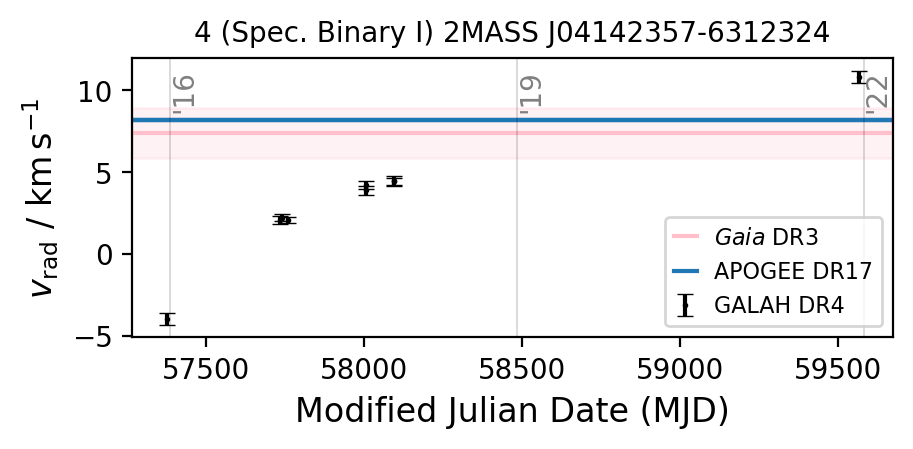
\includegraphics[width=\textwidth]{figures/examples_flag_sp_2.png}
 \caption{\textbf{Example of radial velocity evolution over time for a single-lined spectroscopic binary (SBI)}.}
 \label{fig:examples_flag_sp_2}
\end{figure}

To speed up computation, we use the mean results of the \texttt{allspec} analyses as initial stellar labels for the \texttt{allstar} analysis. All other methodology of the comparison of synthetic spectra to observations (Sec.~\ref{sec:comparison_synthetic_spectra_to_observations} and label optimization (Sec.~\ref{sec:stellar_label_optimization}) apply also to this module, with the exception of the optimization of \logg. Contrary to the \texttt{allspec} approach, we do not fit \logg in this module, but estimate the logarithmic surface gravity $\log g$ using a combination of its definition ($g \propto \frac{\mathcal{M}}{\mathcal{R}^2}$) and the Stefan-Boltzmann law relative to the Solar values:
\begin{equation}
\log g = \log g_\odot + \log \frac{\mathcal{M}}{\mathcal{M_\odot}} + 4 \log \frac{T_\mathrm{eff}}{T_\mathrm{eff,\odot}} - \log \frac{L_\mathrm{bol}}{L_\mathrm{bol,\odot}} \label{eq:logg}
\end{equation}

While we can use our spectroscopically determined $T_\mathrm{eff}$ in Eq. \ref{eq:logg}, the other values have to be estimated through models or non-spectroscopic information. The logarithmic bolometric luminosity, $L_\mathrm{bol}$, can be estimated from the bolometric magnitude, such that $\log \frac{L_\mathrm{bol}}{L_\mathrm{bol,\odot}} = -0.4 \cdot \left(M_\mathrm{bol} - M_\mathrm{bol,\odot} \right)$. The bolometric magnitude can be estimated from any given apparent magnitude, if we correct the latter by the distance modulus, bolometric correction, and extinction. Because essentially all stars in GALAH DR4 have outstanding infrared magnitudes available that suffer less from (uncertain) extinction corrections, we use $K_S$ as the magnitude to estimate our bolometric magnitudes and luminosities via
\begin{equation}
M_\mathrm{bol} = K_S - 5\cdot \log \frac{D_\varpi}{10} + BC(K_S) - A(K_S). \label{eq:mbol}
\end{equation}

While the values for $K_S$, $D_\varpi$, and $A(K_S)$ are readily available (see Sec.~\ref{sec:non-spec_data}), we need to estimate the bolometric correction from tabulated values using the routines provided by \citet{Casagrande2018}:
\begin{equation}
BC(K_S) = f(T_\mathrm{eff}, \log g, \mathrm{[Fe/H]})
\label{eq:bc_ks}
\end{equation}
We choose to assume an extinction value of $E(B-V) = 0\,\mathrm{mag}$ for this particular interpolation and post-correct the value by $A(K_S)$ based on the actual extinctions. The reason for this is that the latter values can exceed the maximum tabulated values of $E(B-V) = 0.72\,\mathrm{mag}$ by \citet{Casagrande2018}.

Because of the appearance of $\log g$ in Eq.~\ref{eq:bc_ks}, we iterate the calculation of $BC(K_S)$ and subsequently $\log g$ up to four times or until the latter value changes less than $0.02\,\mathrm{dex}$ between iterations. Similarly, we need to estimate the stellar masses (and ages as a byproduct) from tabulated values, that is,
\begin{equation}
\mathcal{M}, \tau = f(T_\mathrm{eff}, \log g, \mathrm{[Fe/H]}, L_\mathrm{bol,\odot})
\label{eq:mass_age}
\end{equation}
For this on-the-fly estimate of masses and ages we use an earlier version of the \texttt{ELLI} code by \cite{Lin2018} for a likelihood-weighted estimate with default uncertainties of $100\,\mathrm{K}$, $0.25\,\mathrm{dex}$, $0.2\,\mathrm{dex}$, and an average uncertainty of $L_\mathrm{bol,\odot}$ from propagated uncertainties of Eq.~\ref{eq:mbol}.

We interpolate over the default tables of {\sc parsec+colibri} isochrones \citep{Bressan2012, Marigo2017}, which cover the logarithmic ages of $\log (\tau~/~\mathrm{Gyr}) = 8.00..(0.01)..10.18$ by default and metallicities $\mathrm{[M/H]} = -2.75..(0.25)..-0.75$ as well as $\mathrm{[M/H]} = -0.6..(0.1)..0.7$. We exclude hot stars above $10\,000\,\mathrm{K}$ as well as extremely evolved white dwarf and extremely luminous giant stars ($\log g > 6\,\mathrm{dex}$ or $J - K_S > 2\,\mathrm{mag}$) as they fall far outside our spectroscopic pipeline range. We convert between the theoretical [M/H] and our measured [Fe/H] as well as an assumed $\mathrm{[\upalpha/Fe]}$ enhancement\footnote{We assume $\mathrm{[\upalpha/Fe]} = 0.4$ for $\mathrm{[Fe/H]} < -1$, $\mathrm{[\upalpha/Fe]} = 0.0$ for $\mathrm{[Fe/H]} > 0$ and linearly interpolate between these points for $-1 \leq \mathrm{[Fe/H]} \leq 0$.} via the correlation by \citet{Salaris2006}, $\mathrm{[M/H]} = \mathrm{[Fe/H]} + \log\left(10^{\mathrm{[\upalpha/Fe]}} \cdot 0.694 + 0.306 \right)$. For open clusters with age estimates below $1\,\mathrm{Gyr}$ as well as unevolved stars that are more luminous than expected from the oldest cool main sequence isochrone with matching $\mathrm{[M/H]}$, we sample $\log (\tau~/~\mathrm{Gyr}) = 6.19..(0.01)..10.18$. For globular cluster stars identified in the crossmatch with \citet{Baumgardt2021}, we limit the isochrones to a minimum age of $4.5\,\mathrm{Gyr}$.

\begin{figure*}[ht]
\centering
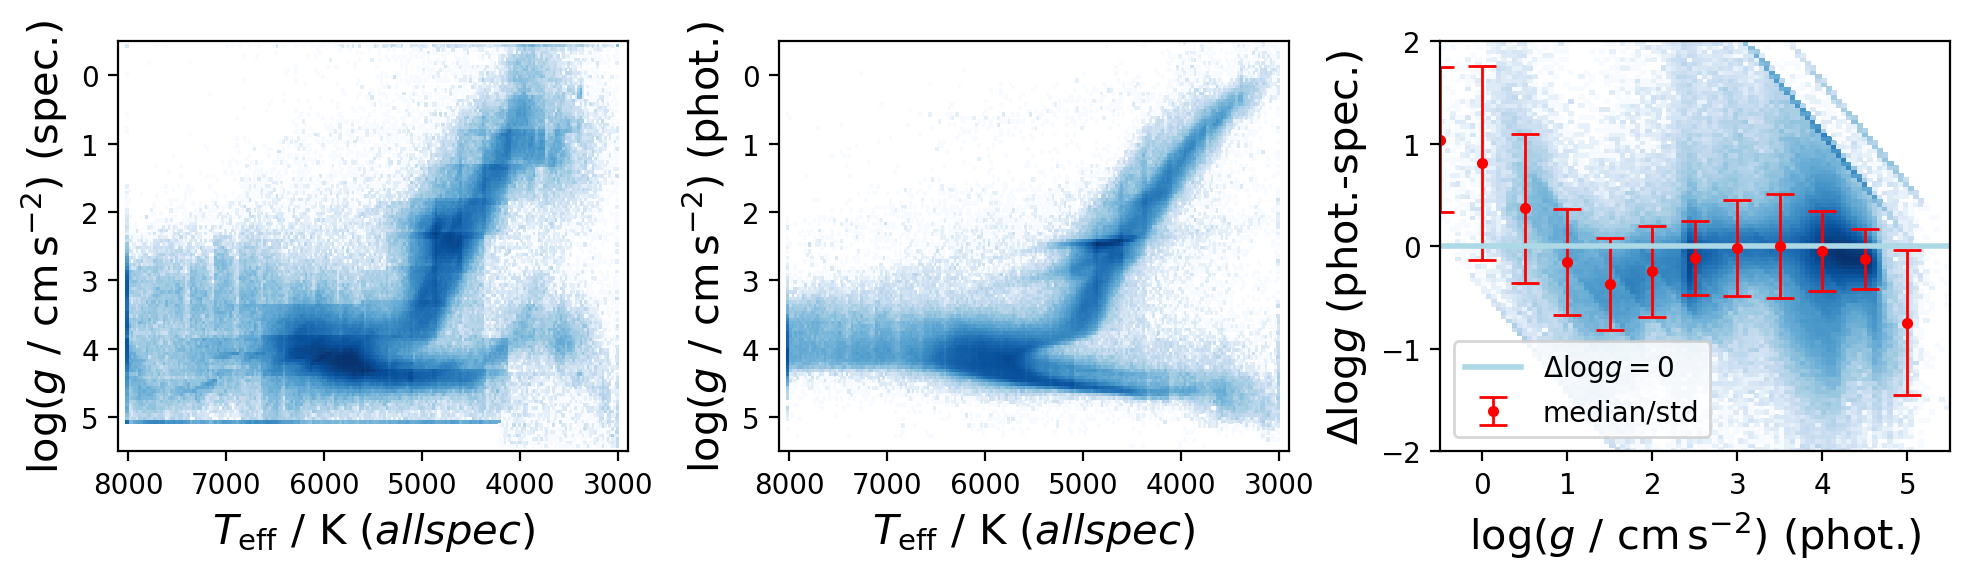
\includegraphics[width=\textwidth]{figures/dlogg_spec_plx.png}
\caption{\textbf{Comparison of spectroscopic and photometric \logg estimates in the \texttt{allspec} analysis}
\textbf{Panel a)} shows the distribution of spectroscopic \logg and \Teff from the \texttt{allspec} module.
\textbf{Panel b)} shows the distribution of the same \Teff and photometric \logg.
\textbf{Panel c)} shows the difference of photometric \logg and spectroscopic \logg as a function of photometric \logg. Red error bars indicate the $1\sigma$ percentiles of this difference in $0.5\,\mathrm{dex}$ bins.}
\label{fig:dlogg_spec_plx}
\end{figure*}

%%%%%%%%%%%%%%%%%%%%%%%%%%%%%%%%%%%%%%%%%%%%%%%%%%%%%%%%%%%%%%%%%%%%%%%%%
\section{POST-PROCESSING}
\label{sec:post_processing}
%%%%%%%%%%%%%%%%%%%%%%%%%%%%%%%%%%%%%%%%%%%%%%%%%%%%%%%%%%%%%%%%%%%%%%%%%

After the \texttt{allspec} and  \texttt{allstar} modules have been run for a night's data (see Secs.~\ref{sec:allspec_analysis} and \ref{sec:allstar_analysis}, respectively), a post-processing routine is used to estimate additional parameters from the residuals of the spectra (Sec.~\ref{sec:residual_analysis}), estimate and validate accuracy and precision uncertainties (Sec.~\ref{sec:uncertainty}), and perform quality assurance tests on a global scale (\texttt{flag\_sp}, see Sec.~\ref{sec:flag_sp}) as well as for the individual abundances of elements X (\texttt{flag\_X\_fe}, see Sec.~\ref{sec:flag_x_fe}).

\subsection{Analysis of spectral residuals} \label{sec:residual_analysis}

\subsubsection{Binary signatures} \label{sec:trigger_binary_module}

The residual spectrum of our best fitting single star analysis can help us to identify a second flux contributor to the observed spectrum. In our case, there are two points in the analysis where we can identify such an influence. Firstly, the residuals are visible in the $\chi^2$ distribution as a function of radial velocity shifts (see Fig.~\ref{fig:181221003101356_single_fit_rv}). While a single star would only show one peak (saved as \texttt{rv\_comp\_1}), a binary system like 2MASS J06084657-7815235 shows a second peak ($-70\,\mathrm{km\,s^{-1}}$ in addition to $74\,\mathrm{km\,s^{-1}}$) that is saved as \texttt{rv\_comp\_2}. Secondly, we perform an automatic search for reoccuring residuals as a function of radial velocity for a few selected lines. We chose the combination of strong lines in the spectra (Balmer lines, Fe lines at 4890 and $4891\,\text{\AA}$, Ni at $6644\,\text{\AA}$) as well as those with the largest expected wavelength shift in the infrared detector (O triplet at $7772-7775\,\text{\AA}$ as well as Mg at $7692\,\text{\AA}$). If we find several peaks with a reasonably similar radial velocity, the likely $X \in {16,50,84}^\text{th}$ percentiles of this radial velocity are saved in \texttt{sb2\_rv\_X}.

Because radial velocities from the \Gaia radial velocity spectrometer \citep{Katz2023} are reported in \Gaia DR3 for 94\% (774\,914) of the stars observed for GALAH DR4, we can also compare against those radial velocity estimates. For 6\% (50\,577) of our stars, we find a difference with respect to \Gaia DR3 larger than $10\,\mathrm{km\,s^{-1}}$. For these stars, as well as stars for which we estimate unrealistic \vmic and \vsini below $0\,\mathrm{km\,s^{-1}}$ in \texttt{allspec}. We note that the \texttt{allspec} analysis was run without boundary conditions for global parameters and thus also resulted in negative velocities, which are later flagged. \texttt{allstar}, however, was run with \vmic and \vsini forced to be above $0\,\mathrm{km\,s^{-1}}$.

\begin{figure*}[ht]
 \centering
 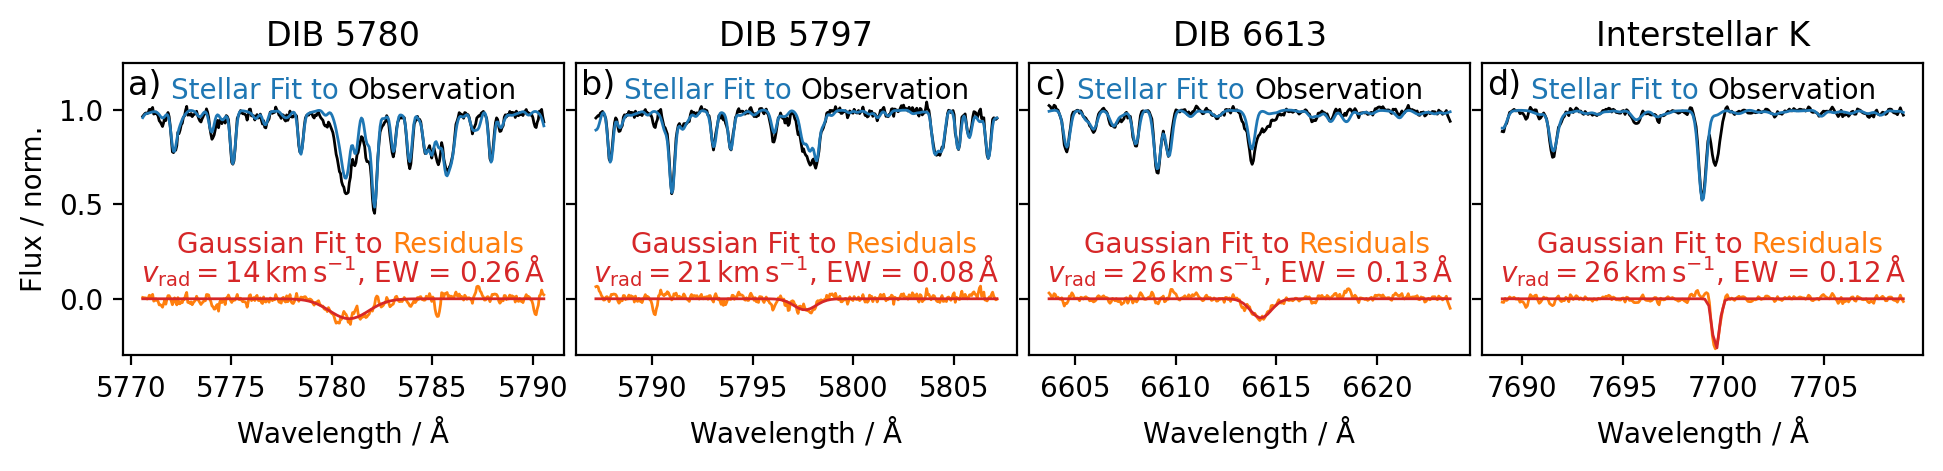
\includegraphics[width=\textwidth]{figures/example_dibs_06453479-0102137.png}
 \caption{\textbf{Example of three diffuse interstellar bands (DIBs) and interstellar K absorption for 2MASS J06453479-0102137 with an $E(B-V) = 0.84\,\mathrm{mag}$ value from \citet{Schlegel1998}.} Shown are the observation (black) and stellar fit (blue) as well as a Gaussian fit (red) to the residual (orange), resulting in an estimate of the equivalent width (EW) as well as radial velocity.} % 140314005201392
 \label{fig:example_dibs_06453479-0102137}
\end{figure*}

\subsubsection{Post-correction of {log\textit{g}} for \texttt{allspec} results}

While we estimate logarithmic surface gravities \logg solely from spectra in the \texttt{allspec} results, we also perform a post-processing estimate where we employ the methodology of Sec.~\ref{sec:allstar_analysis} while fixing all other stellar parameters. The approach of only using spectroscopic information confirmed the previous conclusions of GALAH DR1-DR3 that the spectroscopic information in HERMES spectra to estimate \logg is not sufficient for the majority of the parameter space for the given SNR. We show the spectroscopic \logg in Fig.~\ref{fig:dlogg_spec_plx}a and the photometric \logg and their difference in Figs.~\ref{fig:dlogg_spec_plx}b and c, respectively.

We see an overall good agreement of both \logg estimates for stars between $4250 < T_\text{eff} < 6500\,\mathrm{K}$. Hotter stars show a strong dispersion of spectroscopic \logg due to limited information from fewer and shallower lines. Cooler stars show a significant trend towards much lower \logg for main sequence stars and much higher \logg for cool evolved stars up to an order of $\Delta \log g$ of $1\,\mathrm{dex}$. This trend was previously seen in GALAH DR2 \citep{Buder2018} and is believed to be caused by the onset of molecular absorption features which suppress the continuum for almost the entire HERMES wavelength range (see for example Fig.~\ref{fig:ratio_normalisation}), thus introducing several degeneracies. In addition, we can notice a significantly lower precision of the spectroscopic \logg in comparison to the excellent precision of photometric \logg, for example in the red clump stars.

On closer inspection, we notice several trends in Fig.~\ref{fig:dlogg_spec_plx}a. Most notably, we see noding patterns along the \Teff and \logg grids where the \texttt{allspec} module switches between different neural network models. Our investigation of these noding effects is addressed in Sec.~\ref{sec:caveats}. In comparison to Fig.~\ref{fig:dlogg_spec_plx}b, where a clear equal-mass binary sequence is visible just above the cool main sequence, we do not see such a sequence in Fig.~\ref{fig:dlogg_spec_plx}a. The difference between spectroscopic and photometric \logg will therefore be useful to identify photometric binaries at least for the high quality spectra (where \logg precisions are below the single to binary system offset of $\Delta \log g = 0.3\,\mathrm{dex}$), as discussed in Sec.~\ref{sec:flag_sp}.

\subsubsection{Interstellar absorption}

Because we can create synthetic stellar spectra for the full wavelength range, we can now also trace interstellar absorption in the residuals of observed spectra. By default, we try to calculate the equivalent width via Gaussian fits to the three diffuse interstellar bands (5780.59, 5797.19, 6613.66\Angstroem) with central wavelengths identified by \citet{Vogrincic2023} as well as for interstellar K ($7698.9643\,\text{\AA}$), see Fig.~\ref{fig:example_dibs_06453479-0102137}. We report the equivalent widths \texttt{eq\_x}, standard deviations \texttt{sigma\_x} and radial velocities \texttt{rv\_x} for \texttt{x} in \texttt{k\_is} for interstellar K and \texttt{x} in \texttt{DIB\_5780}, \texttt{DIB\_5797}, and \texttt{DIB\_6613} for the DIBs. The coverage of interstellar material, estimated from \texttt{DIB\_5780}, within $D_\varpi < 5\,\mathrm{kpc}$ is shown in an all-sky map in Fig.~\ref{fig:galah_dr4_dibs_gaia_dr3_extinction}, with the GSPhot extinction by \citet{Andrae2023} in the background.

\begin{figure}[ht]
 \centering
 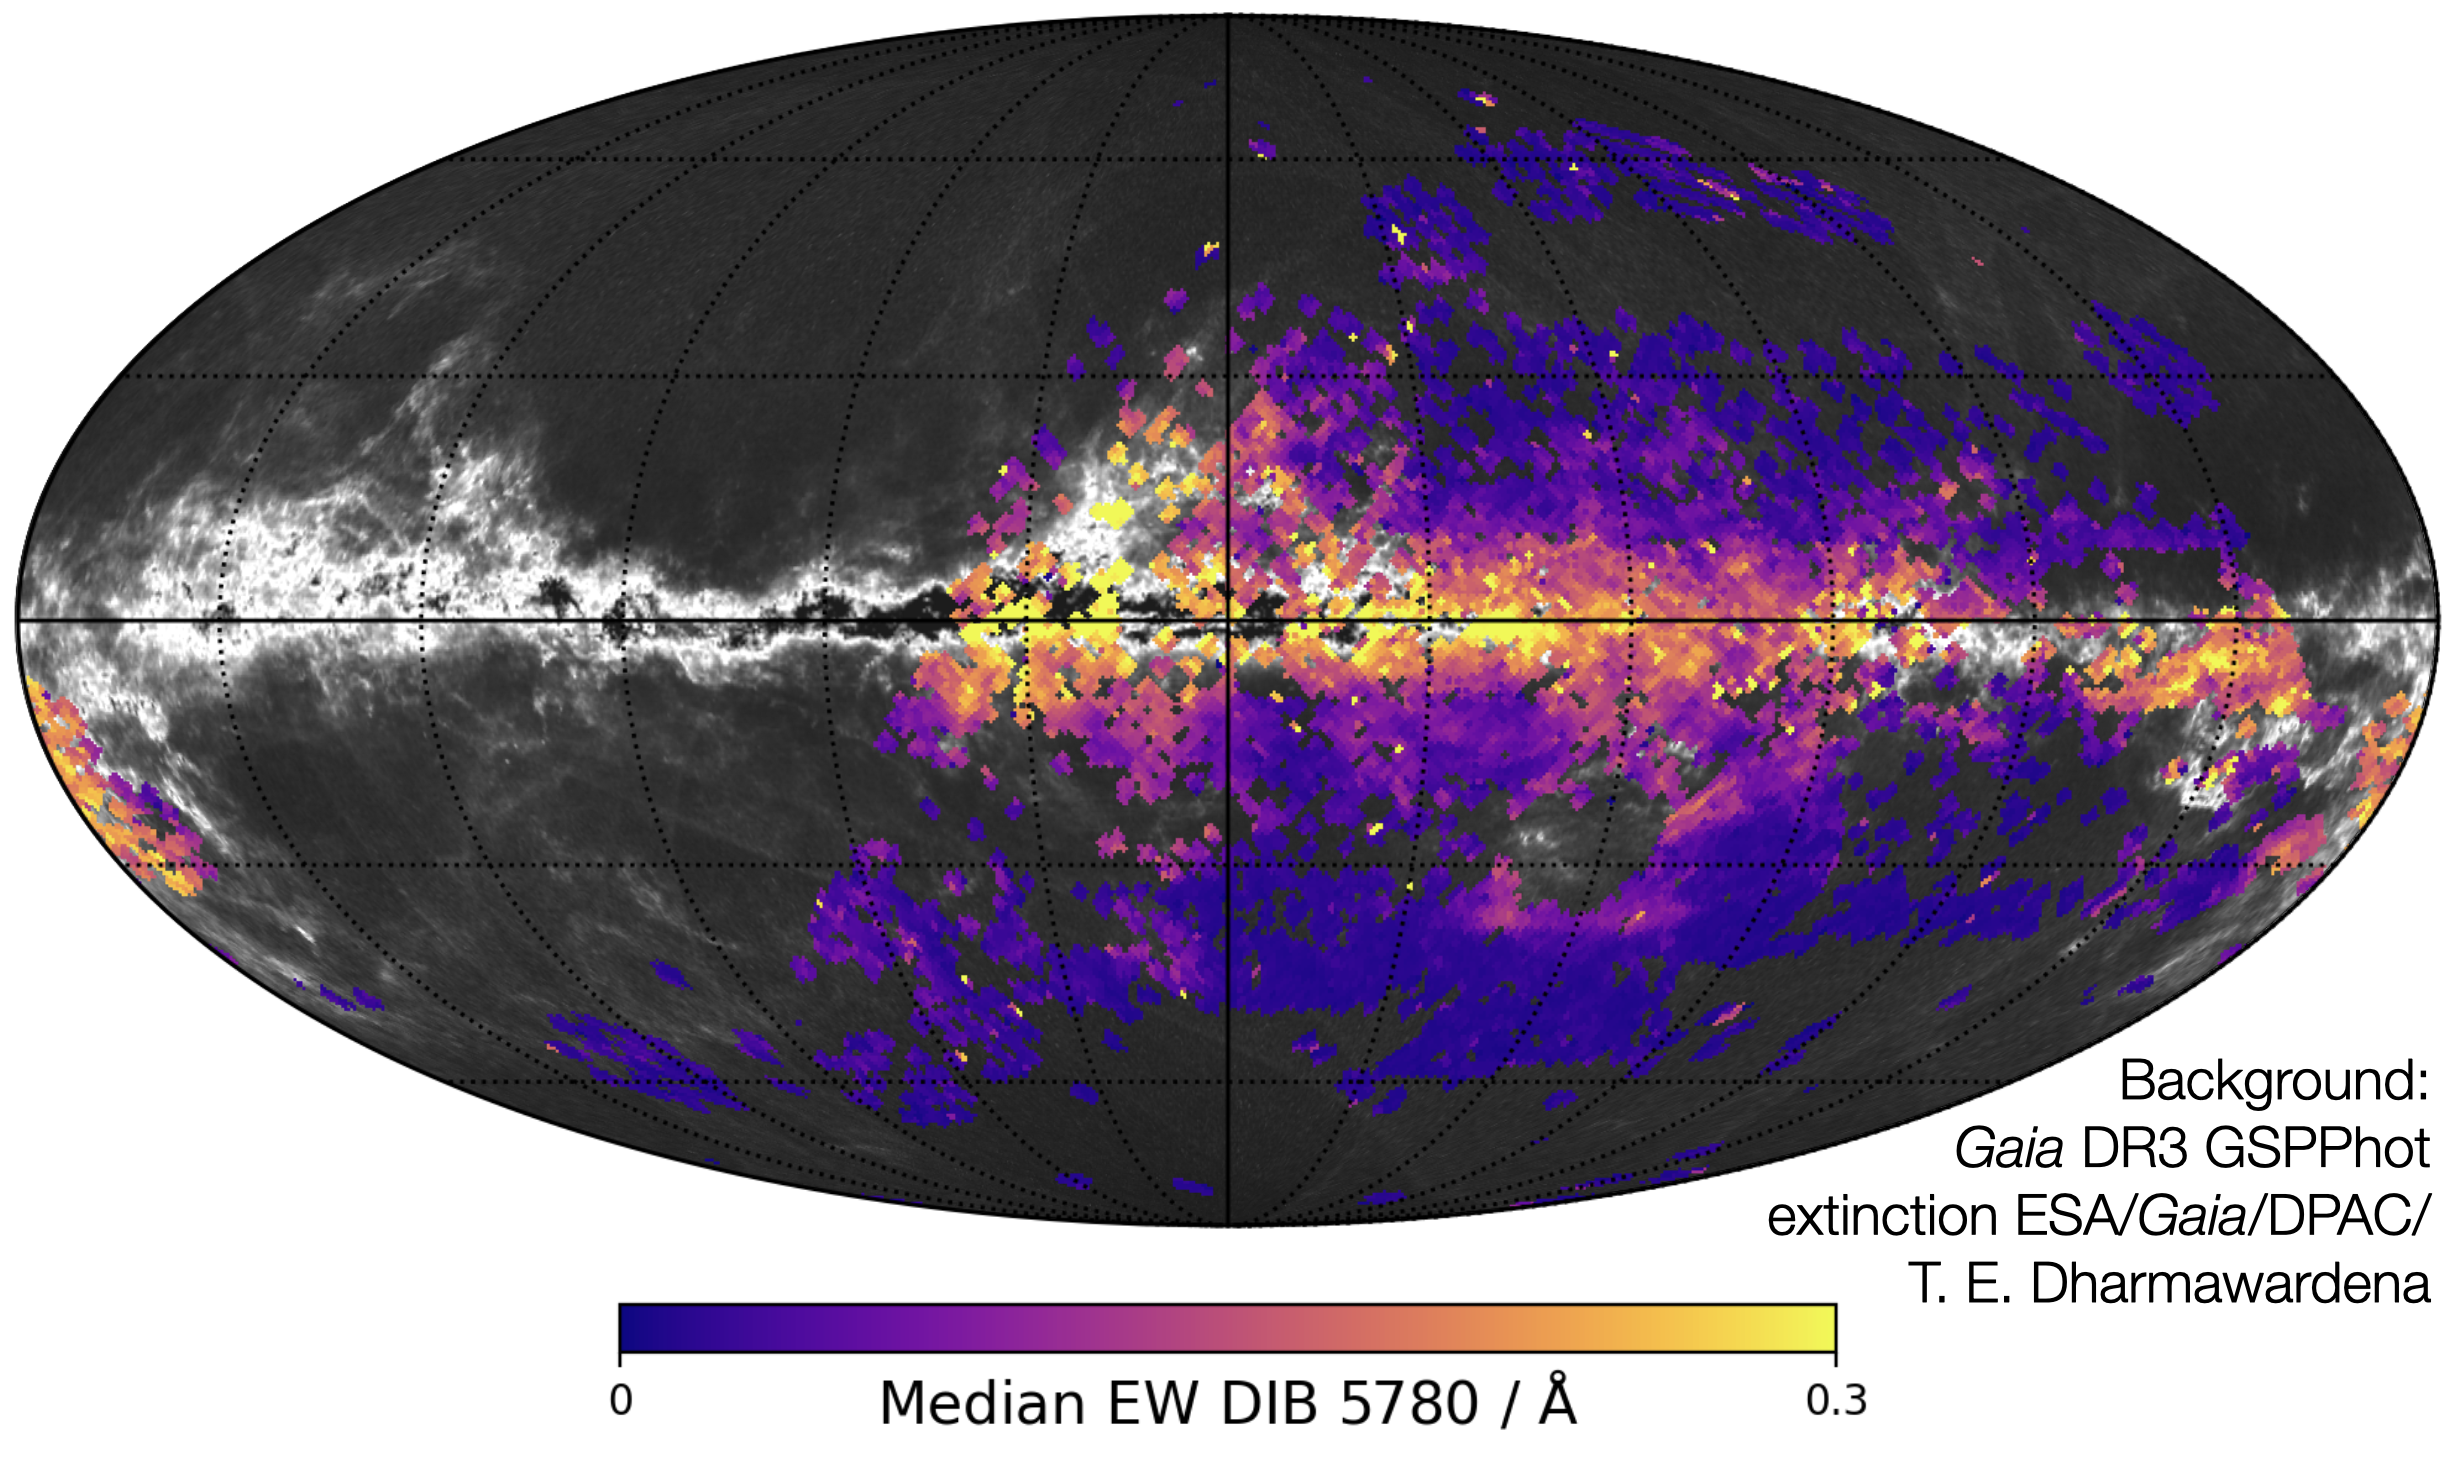
\includegraphics[width=\textwidth]{figures/galah_dr4_dibs_gaia_dr3_extinction.png}
 \caption{\textbf{All-sky map (l,b) of GALAH DR4 equivalent width measurements of the diffuse interstellar band around 5780\,\AA, with the GSPhot extinction by \citet{Andrae2023} in the background.}}
 \label{fig:galah_dr4_dibs_gaia_dr3_extinction}
\end{figure}

\begin{figure}[ht]
 \centering
 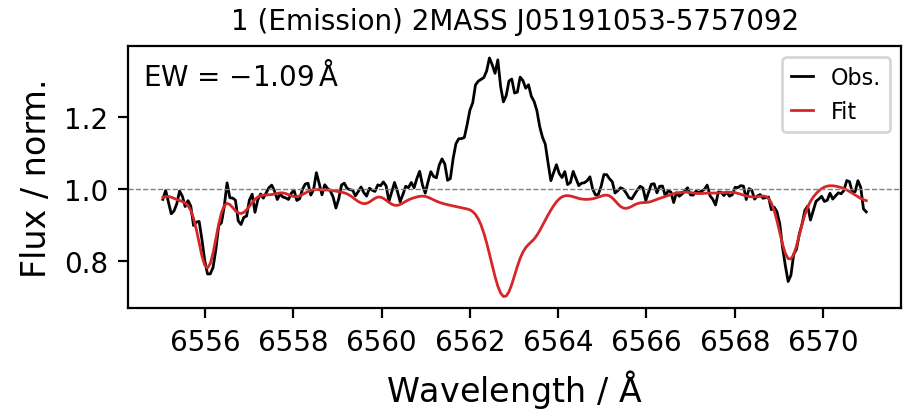
\includegraphics[width=\textwidth]{figures/examples_flag_sp_1.png}
 \caption{\textbf{Example of a star with clear emission in the Balmer lines (here $\mathrm{H_\upalpha}$). The bit indicating emission has been raised in the major quality flag \texttt{flag\_sp} for this star.}} \label{fig:examples_flag_sp_1}
\end{figure}

\subsubsection{Emission estimates for the Balmer lines}

The difference between synthetic and observed Balmer line absorption holds valuable information on active stars, as well as the known inaccuracy of the synthetic Balmer lines, as well as masses for evolved stars \citep{Bergemann2016} and possibly even information on unresolved binary systems \citep{Sayeed2024}. We therefore perform a trapezoidal integration around the Balmer lines at $4861.3230$ and $6562.7970\,\text{\AA}$ whose values we report in \texttt{ew\_h\_beta} and \texttt{ew\_h\_alpha}. By default we integrate in a window of $\pm 0.75$ and $1.25\,\text{\AA}$ for $\text{H}_\upbeta$ and $\text{H}_\upalpha$, respectively, and increase this window to $5\,\text{\AA}$ if the average observed, normalised flux within $\pm 0.5\,\text{\AA}$ of the Balmer line core exceeds 1. An example of such a star is shown in Fig.~\ref{fig:examples_flag_sp_1}, for which we measure a residual EW of $1.09\,\text{\AA}$. Most emission line stars in the GALAH sample are found the the region of pre-main-sequence and hot stars (see Fig.~\ref{fig:flag_sp_overview_allstar}a).


\begin{figure*}[ht]
 \centering
 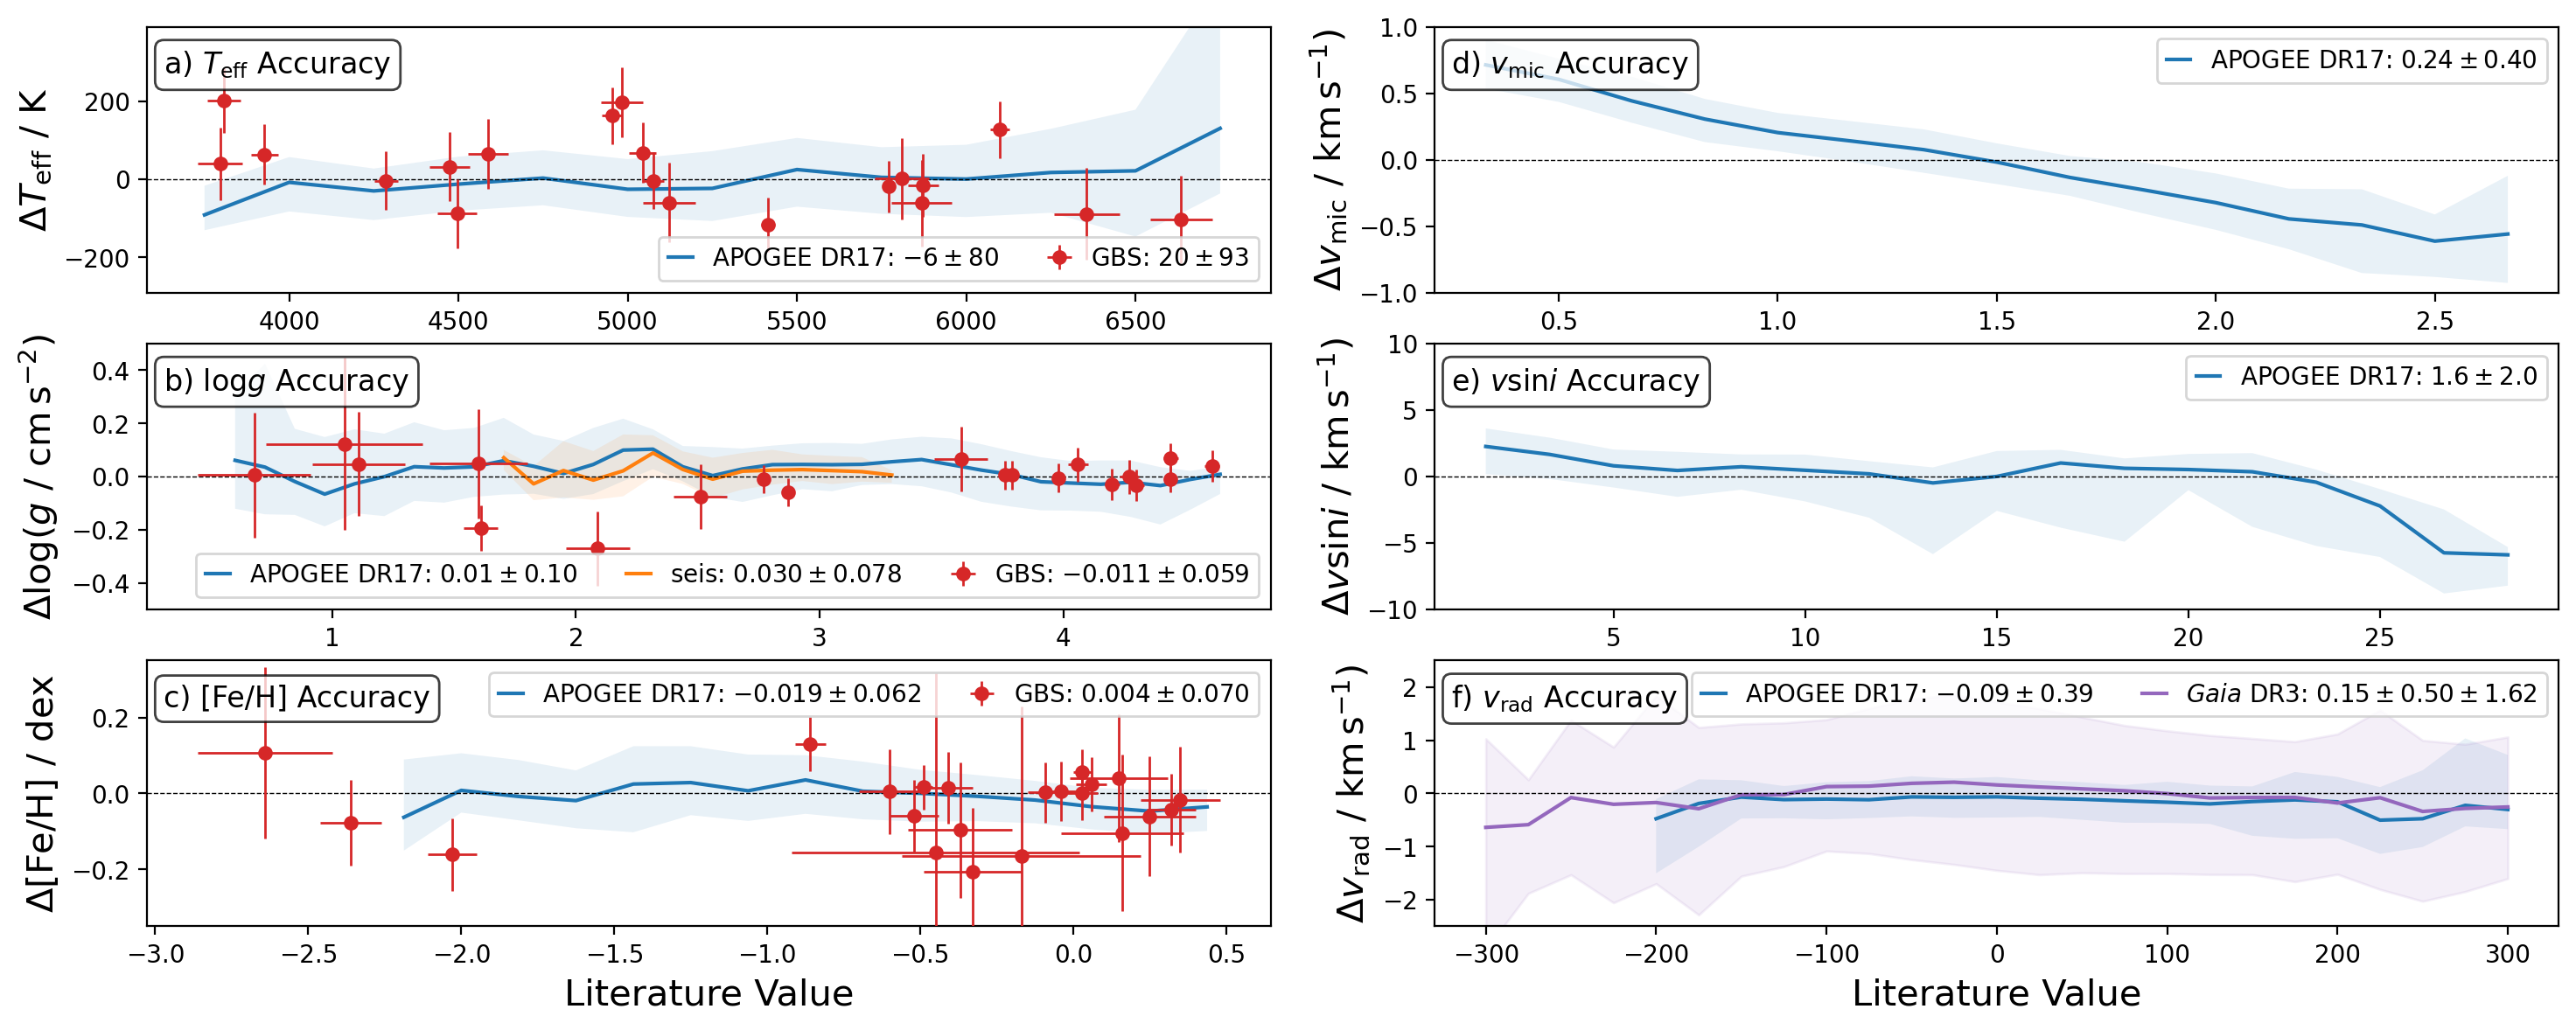
\includegraphics[width=\textwidth]{figures/galah_dr4_validation_parameter_accuracy_allstar.png}
 \caption{\textbf{Accuracy of the main stellar parameters \Teff, \logg, \feh, \vmic, \vsini, and \vrad for GALAH DR4.}. Each panel shows the comparison to literature (DR4 - literature). Comparisons are performed for the \Gaia FGK Benchmark stars (red), APOGEE DR17 (blue), \logg inferred from asteroseismic measurements (orange) and \Gaia DR3 radial velocities (purple).}
 \label{fig:galah_dr4_validation_parameter_accuracy_allstar}
\end{figure*}

%%%%%%%%%%%%%%%%%%%%%%%%%%%%%%%%%%%%%%%%%%%%%%%%%%%%%%%%%%%%%%%%%%%%%%%%%
\subsection{Uncertainty estimation and validation}
\label{sec:uncertainty}
%%%%%%%%%%%%%%%%%%%%%%%%%%%%%%%%%%%%%%%%%%%%%%%%%%%%%%%%%%%%%%%%%%%%%%%%%

The uncertainties that we report for our spectroscopic data analysis are based on the comparison to literature measurements to estimate accuracy uncertainties and a combined precision uncertainty estimate from adjusted covariance estimates of the fitting process and the scatter of repeat observations. Formally, we estimate the total variance of measurements as a combination of the accuracy and precision variance

\begin{align} \label{eq:total_uncertainty}
    \sigma_\mathrm{total}^2 = \sigma_\mathrm{accuracy}^2 + \sigma_\mathrm{precision}^2
\end{align}

Representative values of accuracy and precision for our stellar parameters are listed in Table~\ref{tab:accuracy_precision}. In the following sections, we lay out how we estimate and validate accuracy and precision uncertainties in Secs.~\ref{sec:uncertainty_accuracy} and \ref{sec:uncertainty_precision}, respectively.

\begin{table}[ht]
\centering
\caption{List of accuracy and representative precision uncertainties for stellar parameters in GALAH DR4. Accuracy values are estimated from comparisons with literature references (see Sec.~\ref{sec:uncertainty_accuracy}), whereas precision estimates are estimated from covariance uncertainties and repeat observations (Secs.~\ref{sec:uncertainty_precision}). Here, we list the median precision uncertainties for stars with $SNR = 50 \pm 10$ in CCD2 (see Fig.~\ref{fig:galah_dr4_precision_parameters}).}
\label{tab:accuracy_precision}
\begin{tabular}{ccc}
\hline \hline
Parameter / Unit & Accuracy & Precision ($SNR = 50$)\\
\hline
$T_\text{eff}~/~\mathrm{K}$          & 66     & $23 \pm 5$ \\
$\log (g~/~\mathrm{cm\,s^{-2}})$     &  0.042 & -- \\
$\mathrm{[Fe/H]}~/~\mathrm{dex}$     &  0.051 & $0.025 \pm 0.004$ \\
$v_\text{mic}~/~\mathrm{km\,s^{-1}}$ &  0.28  & $0.05 \pm 0.03$ \\
$v \sin i~/~\mathrm{km\,s^{-1}}$     &  1.4   & $0.5 \pm 0.2$ \\
$v_\text{rad}~/~\mathrm{km\,s^{-1}}$ &  0.15  & $0.17 \pm 0.02$ \\
\hline
\end{tabular}
\end{table}

\subsubsection{Accuracy estimation and validation} \label{sec:uncertainty_accuracy}

Estimating the accuracy of spectroscopic measurements has always been a complicated endeavour, because there are no universal benchmark sets for all parameters across all stellar types yet. Subsequently, we describe the numerous comparisons that we have performed for both stellar parameters (\Teff, \logg, \feh, \vmic, \vsini, and \vrad) as well as the elemental abundance measurements. Consistent with GALAH DR3 \citep{Buder2021}, and caused by the limited coverage of benchmark literature, we continue to use a single accuracy estimate for each stellar parameter and ignore the possibly large accuracy uncertainties for the elemental abundances. In all cases, we do estimate an overall bias with respect to literature values and then combine these estimates to a globally applied zeropoint correction. Where not explicitly stated otherwise, we use assume that the spread of stellar parameters residuals is indicative of the accuracy of either method and estimate our accuracy by dividing the parameter spread by $\sqrt{2}$. The applied shifts are listed in Table~\ref{tab:zeropoints}. We estimate the accuracy and bias correction for stellar parameters (including the iron abundance as a global parameter) and abundances separately.

Our primary reference source for parameter accuracy remain the \Gaia FGK benchmark stars \citep{Jofre2014, Jofre2015, Jofre2018, Heiter2015}. Additionally, we use estimates from asteroseismic estimates of the K2 and TESS photometry \citep{Zinn2020, Hon2021} to compare our surface gravities and perform a validation to higher quality observations of globular cluster stars with typically lower metallicities \citep{Carretta2009c, Carretta2009, Johnson2010}. Because the overlap with APOGEE DR17 \citep{SDSSDR17} has increased from 41\,941 stars in GALAH DR3 to 60\,046 stars with 92\,368 repeat observation matches in GALAH DR4, we also can assess systematic trends for a larger parameter space. For clarity, we discuss the stellar parameters separately, but show most accuracy estimates in a combined figure Fig.~\ref{fig:galah_dr4_validation_parameter_accuracy_allstar}.

\Teff: The effective temperature estimates from GALAH DR4 show good agreement with the \Gaia FGK benchmark stars (Fig.~\ref{fig:galah_dr4_validation_parameter_accuracy_allstar}a). Specifically, we find a mean difference of $\Delta T_\mathrm{eff} = 21 \pm 92\,\mathrm{K}$, indicating no significant bias between our temperatures and the benchmark values. Comparisons with APOGEE DR17 show an equally robust agreement, with $\Delta T_\mathrm{eff} = -8 \pm 78\,\mathrm{K}$. This small offset and uncertainty suggest that the GALAH DR4 \Teff estimates are highly reliable across a wide range of at least G- and K-, but possibly also F- and M-type stars. Here, we use $1/\sqrt{2}$ of the residual spread with respect to \Gaia benchmark stars as our accuracy estimate.

\logg: For surface gravity, we compared our \logg estimates to both the \Gaia FGK benchmark stars, asteroseismic measurements from \citet{Zinn2020} and \citet{Hon2021}, and APOGEE DR17. The asteroseismic \logg values are derived from $\nu_\mathrm{max}$ measurements for giant stars, and they show excellent agreement with our results, with a mean difference of $\Delta \log g = 0.026 \pm 0.078$. Both the asteroseismic comparison as well as the \Gaia benchmark star comparison ( $\Delta \log g = -0.011 \pm 0.059$) and APOGEE DR17 ($\Delta \log g = 0.00 \pm 0.10$) agree well and show no trends across the \logg range. This is a significant improvement over GALAH DR3, were significant deviations were found for luminous giant stars - whose parameter estimates in GALAH DR3 suffered from less precise and systematically biased distance and thus \logg estimates. We do find significant outliers, however, particularly for primary red clump stars, which were mistaken as secondary red clump stars, leading to larger deviations. We discuss this issue later in Sec.~\ref{sec:caveats_photospec}. Because this single group is driving the scatter of our disagreement with the asteroseismic estimates, we revert to the \Gaia benchmark stars to estimate the accuracy.

\begin{figure}[ht]
 \centering
 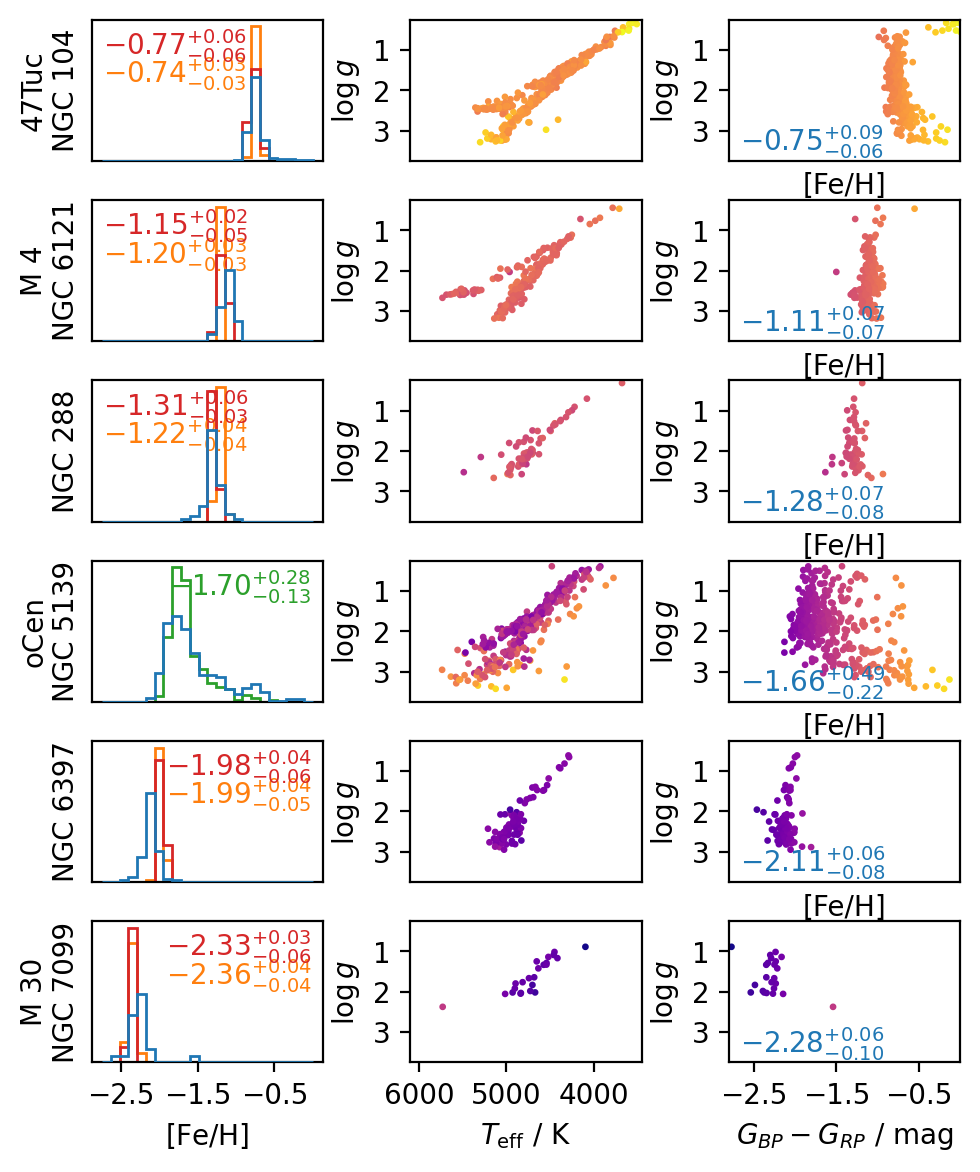
\includegraphics[width=\columnwidth]{figures/galah_dr4_allstar_globular_cluster_feh_comparison.png}
 \caption{\textbf{Comparison of iron abundances (16th, 50th and 84th percentiles) and overview of spectroscopic and photometric properties of globular cluster stars in GALAH DR4.}
 \textbf{Left panels} show histograms of iron abundances from GALAH DR4 (blue) as well as literature estimates for the globular clusters from Giraffe (orange) and UVES (red) observations by \citep{Carretta2009c, Carretta2009} as well as observations from \cite{Johnson2010}.
 \textbf{Middle panels} show the spectroscopic \Teff-\logg diagrams colored by iron abundance \feh.
 \textbf{Right panels} show the trend of GALAH DR4 [Fe/H] along the different \logg values.
}
 \label{fig:galah_dr4_allstar_globular_cluster_feh_comparison}
\end{figure}

\feh: The comparison of GALAH DR4 metallicities to the \Gaia FGK benchmark stars initially showed the similar bias of GALAH towards more metal-poor values on the $0.049\,\mathrm{dex}$ level. The application of a zeropoint correction (see Table~\ref{tab:zeropoints}) yields an excellent agreement, with $\Delta \mathrm{[Fe/H]} = 0.004 \pm 0.067$ for the benchmark stars and $\Delta \mathrm{[Fe/H]} = -0.022 \pm 0.061$ for APOGEE DR17, confirming the reliability of the GALAH DR4 metallicity estimates across a large range of metallicities. For the metal-poor regime, benchmark estimates are still rare. Luckily, a dedicated observing program -- whose results are included in this data release -- was performed and an overview of globular cluster Kiel diagrams is appended in Fig.~\ref{fig:galah_dr4_gcs_teff_logg}. We therefore only perform a comparison with globular cluster stars -- often measured in 1D LTE -- to get a quantitative impression of the agreement. We restrict ourselves to a few studies, namely those by \citet{ Carretta2009c, Carretta2009} for NGCs 104, 6121, 288, 6397, and 7099 as well as \citet{Johnson2010} for NGC 5139. In all cases, we find a good agreement of the metallicity distribution function for overlapping stars within the uncertainties (see Fig.~\ref{fig:galah_dr4_allstar_globular_cluster_feh_comparison}). While this is not necessarily confirming our accuracy, it is showing consistency within this uncertain parameter regime. We note however, a specific region in NGC~104, where the metallicity of the most luminous giants ($T_\mathrm{eff} < 3750\,\mathrm{K}$ and $\log g < 0.5$) is incorrectly estimated near the Solar value. We discuss this problem in detail as a caveat in Sec.~\ref{sec:caveats_fitting}, since we have not been able to systematically flag these stars. More generally, we note that the strong and unexpected abundance trends with \Teff or \logg in globular clusters from GALAH DR3 have decreased for most elements. A custom analysis of globular cluster abundances beyond [Fe/H] will be performed in a dedicated study (McKenzie et al., in preparation), as these observations have been part of a dedicated observing program (PIs M. McKenzie and M. Howell). Similarly, a dedicated verification of open cluster observations (PIs J. Kos and G. De Silva) will be performed in a separate study (Kos et al., in preparation).

\vmic: Microturbulence velocities show a more complex pattern when compared to APOGEE DR17. We find a mean difference of $\Delta v_\mathrm{mic} = 0.23 \pm 0.39\,\mathrm{km\,s^{-1}}$. However, the comparison reveals a linear mismatch: APOGEE DR17 tends to measure lower \vmic values for stars with low microturbulence and larger \vmic values for stars with higher microturbulence compared to GALAH DR4. This systematic trend suggests that the \vmic calibration between the two surveys may differ slightly, particularly at the extremes of the parameter range. We note, however, that the surveys agree much better than for GALAH DR3, where a fixed quadratic relation was used that did not allow for deviations, for example for red clump stars. Fitting \vmic returned a similar pattern as the empirical relation by \citet{DutraFerreira2016} and show a significantly different behaviour of \vmic for the hottest, coolest, and red clump stars (see Fig.~\ref{fig:initial_parameters}). This mismatch of \vmic could have indeed driven the metallicity mismatch of metal-rich red clump stars in GALAH DR2 and DR3 \citep{Buder2018, Buder2021}, since their metallicities are in agreement with other estimates now (e.g. APOGEE DR17).

\begin{figure*}[ht]
 \centering
 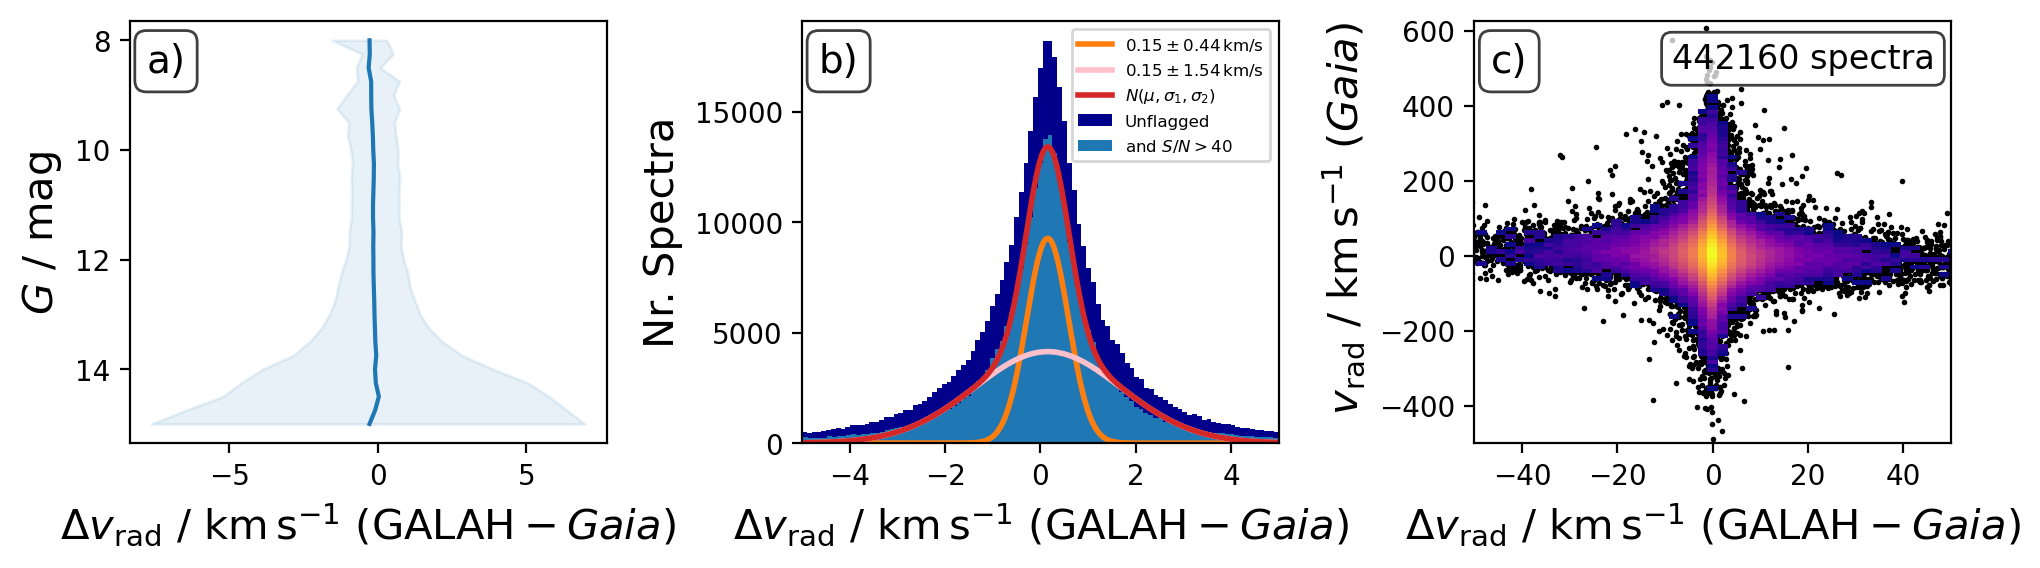
\includegraphics[width=\textwidth]{figures/galah_dr4_vrad_gaia_dr3.png}
 \caption{\textbf{Comparison of radial velocities between GALAH DR4 \texttt{allspec} and \Gaia DR3.}
 \textbf{Panel a)} shows the difference of radial velocities as function of \Gaia $G$ magnitude.
 \textbf{Panel b)} shows a histogram of the difference with two Gaussian distributions (with same mean) fitted to them to estimate a more robust, that is binary independent, radial velocity difference.
 \textbf{Panel c)} shows the difference of radial velocities as function of radial velocity, showing the systematic scatter introduced by binaries.
}
 \label{fig:galah_dr4_vrad_gaia_dr3}
\end{figure*}

\vsini: The rotational velocity estimates agree well with APOGEE DR17, with a mean difference of $\Delta v \sin i = 1.6 \pm 2.0\,\mathrm{km\,s^{-1}}$. However, at higher rotational velocities (above approximately $24\,\mathrm{km\,s^{-1}}$), our neural networks are starting to extrapolate, leading to an upper limit in the estimates and returning significantly lower \vsini values compared to APOGEE DR17. This issue highlights the limitations of the GALAH DR4 \vsini estimates for rapidly rotating stars.

\vrad: For radial velocity we compared our results to both APOGEE DR17 and \Gaia DR3. The comparison with APOGEE DR17 yields a small offset of $\Delta v_\mathrm{rad} = -0.09 \pm 0.39\,\mathrm{km\,s^{-1}}$, indicating excellent agreement between the two surveys. Accounting for the much lower SNR for faint \Gaia targets and unidentified binaries, we are fitting two Gaussian distributions to the overall difference of GALAH and \Gaia radial velocities (see Fig.~\ref{fig:galah_dr4_vrad_gaia_dr3}). The comparison with Gaia DR3 shows a slightly larger offset of $\Delta v_\mathrm{rad} = 0.15 \pm 0.44 \pm 1.54\,\mathrm{km\,s^{-1}}$, which is expected due to the lower precision of the \Gaia DR3 radial velocities \citep{Katz2023}. We use the median residual of $0.15\,\mathrm{km\,s^{-1}}$ with respect to \Gaia DR3 rather than the spread as our accuracy estimate.

Elemental abundances [X/Fe]: While there is no model-independent benchmark for abundance accuracy, we continue to perform a variety of comparisons with literature measurements to at least analyse the consistency with other estimates. In GALAH DR4, we analyse the overall zeropoints of abundances with up to five different estimates (see Fig.~\ref{fig:galah_dr4_zeropoint_checks_allstar}): (1) the spectroscopic analysis of a spectrum with solar composition of the asteroid 4 Vesta (210115002201239), (2) the abundance estimate from Solar twins for an Solar age of $4.5\,\mathrm{Gyr}$ (see Fig.~\ref{fig:galah_dr4_age_xfe_trends_solar_twins_allstar}), (3) the abundances estimates of \Gaia FGK benchmark stars \citep{Jofre2015, Jofre2018}, (4) the stars with Solar-like metallicity $-0.1 < \mathrm{[Fe/H]} < 0.1$ in the Solar neighbourhood of $D_\varpi < 500\,\mathrm{pc}$ \citep[a method introduced by][]{Joensson2020}, and (5) the abundance difference of stars overlapping with the high-resolution large scale spectroscopic APOGEE DR17 \citep{SDSSDR17}. We stress that our abundance corrections and as a consequence thereof our Solar abundances in Table~\ref{tab:zeropoints}, are estimated in 1D LTE or 1D NLTE and do not represent the most accurate Solar abundances, but merely reflect our rather best attempt to minimise the disagreement of abundances for a variety of cases. For several science cases, an adjustment of the abundance zeropoints might be advisable.

While we are not able to include all of our validation plots, we refer the interested reader to the publicly available code in our code repository\footnote{\url{https://github.com/svenbuder/GALAH_DR4/tree/main/validation}}. Generally speaking, we have found that a large number of systematic trends of abundances with temperature and surface gravity has decreased with respect to GALAH DR3, as can be appreciated from dedicated validation plots (\href{https://github.com/svenbuder/GALAH_DR4/blob/main/validation/galah_dr4_validation_globular_clusters.ipynb}{online here}) -- with a similar appearance as the right hand panels of Fig.~\ref{fig:galah_dr4_allstar_globular_cluster_feh_comparison}.

\begin{figure*}[ht]
 \centering
 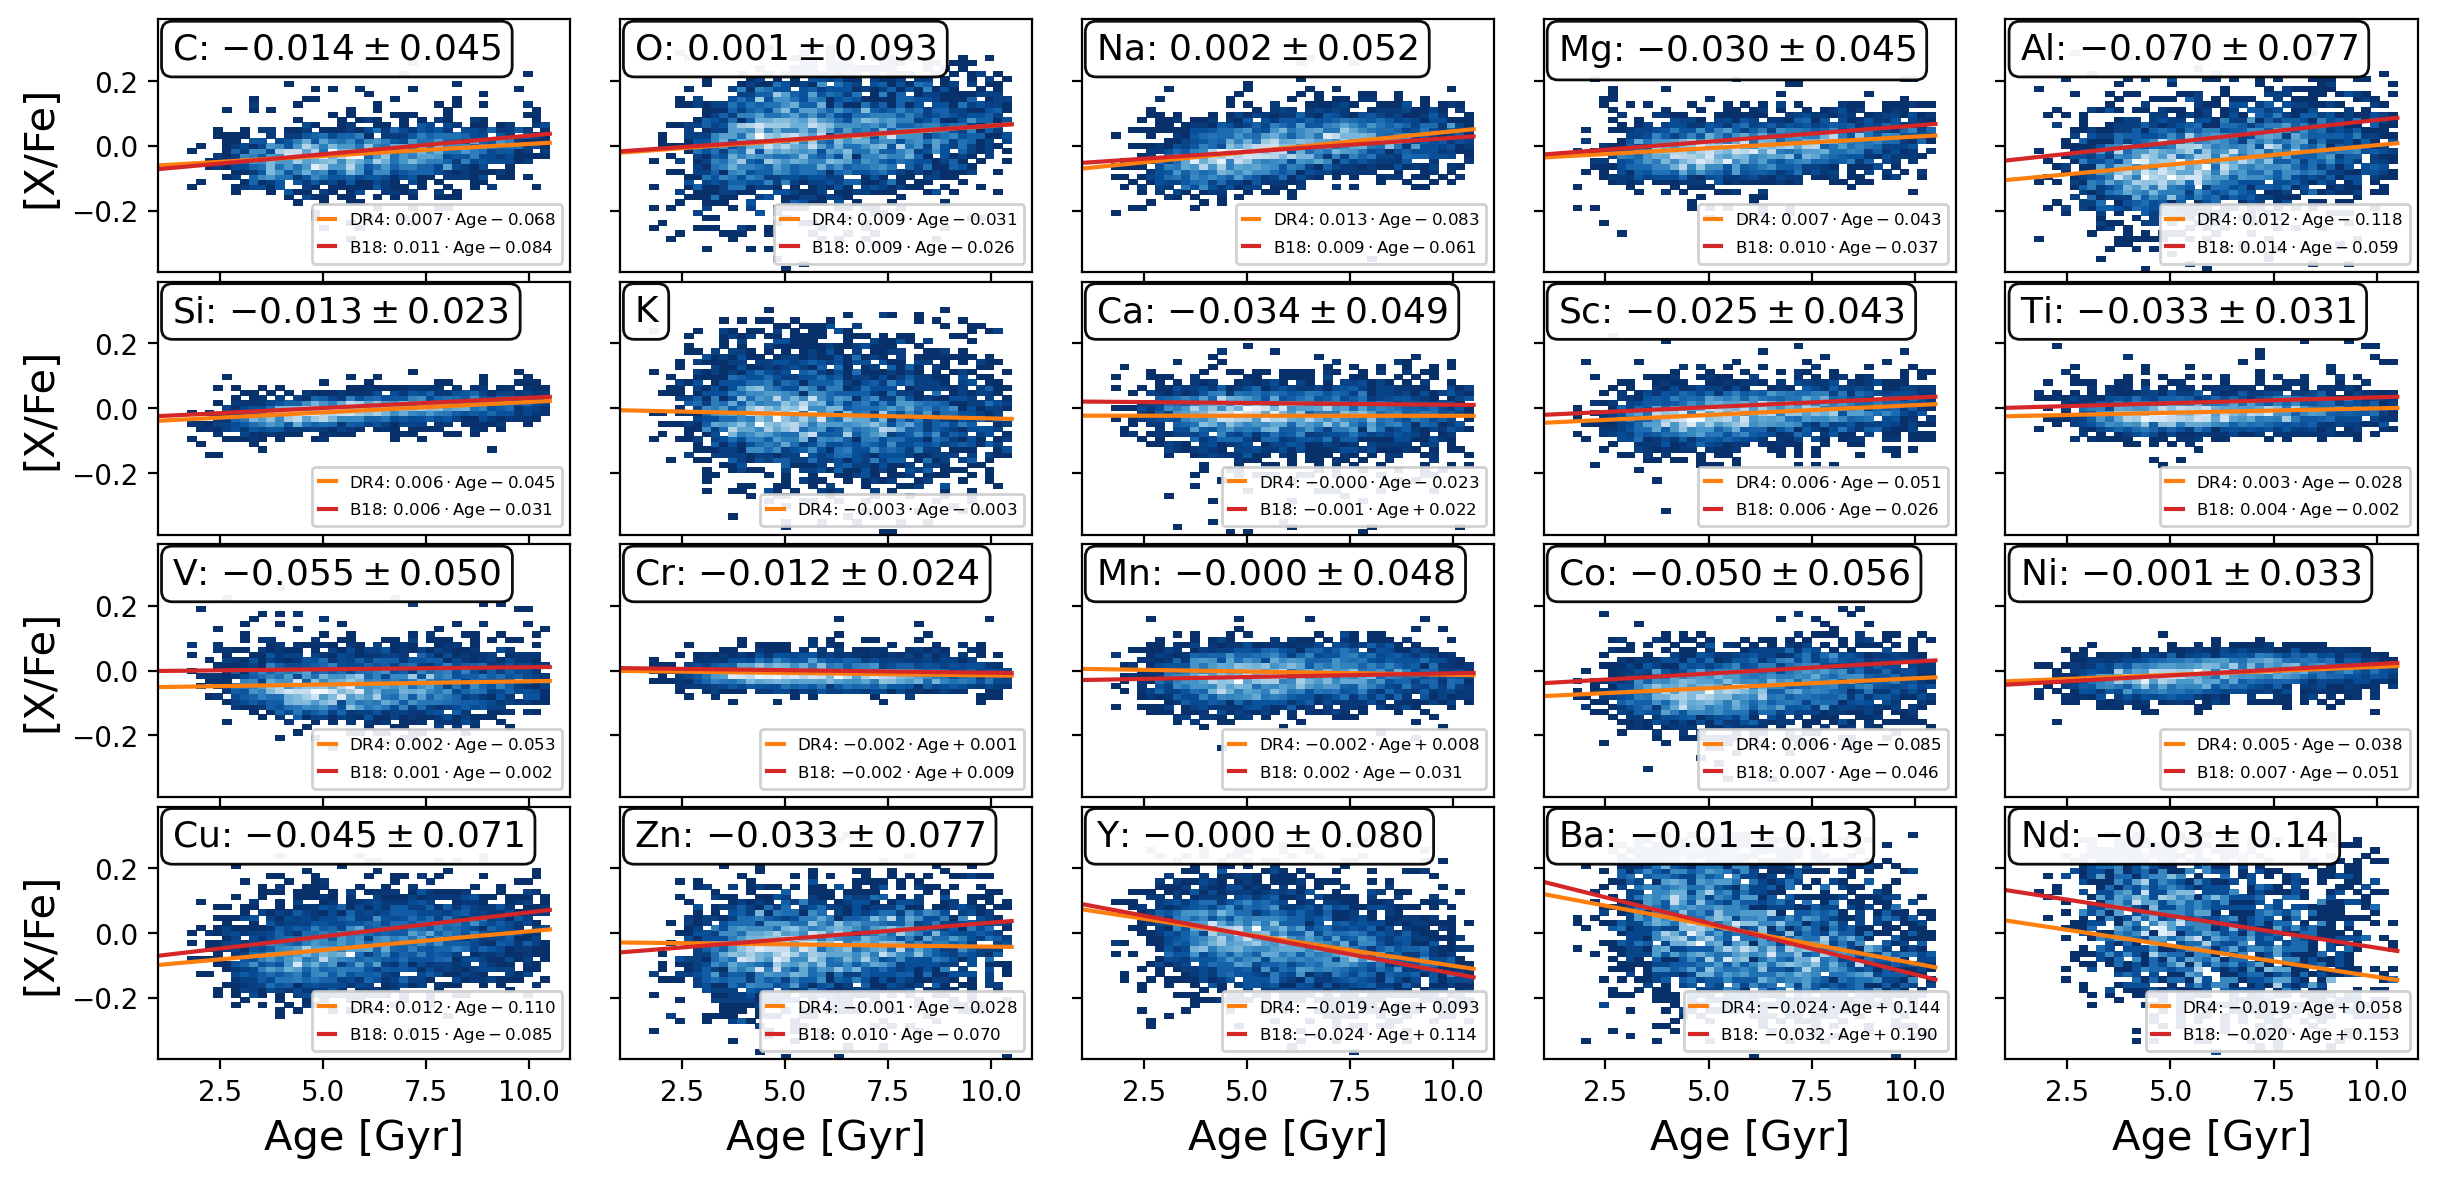
\includegraphics[width=\textwidth]{figures/galah_dr4_age_xfe_trends_solar_twins_allstar.png}
 \caption{\textbf{Chemical abundances [X/Fe] of Solar twin stars as a function of ages that were estimated as part of the mass and age estimation of the allstar spectrum analysis.} We overplot linear fits to our age-abundance relations for Solar twins in orange as well as the literature values from \citet{Bedell2018} in red.}
 \label{fig:galah_dr4_age_xfe_trends_solar_twins_allstar}
\end{figure*}

\begin{figure}[ht]
 \centering
 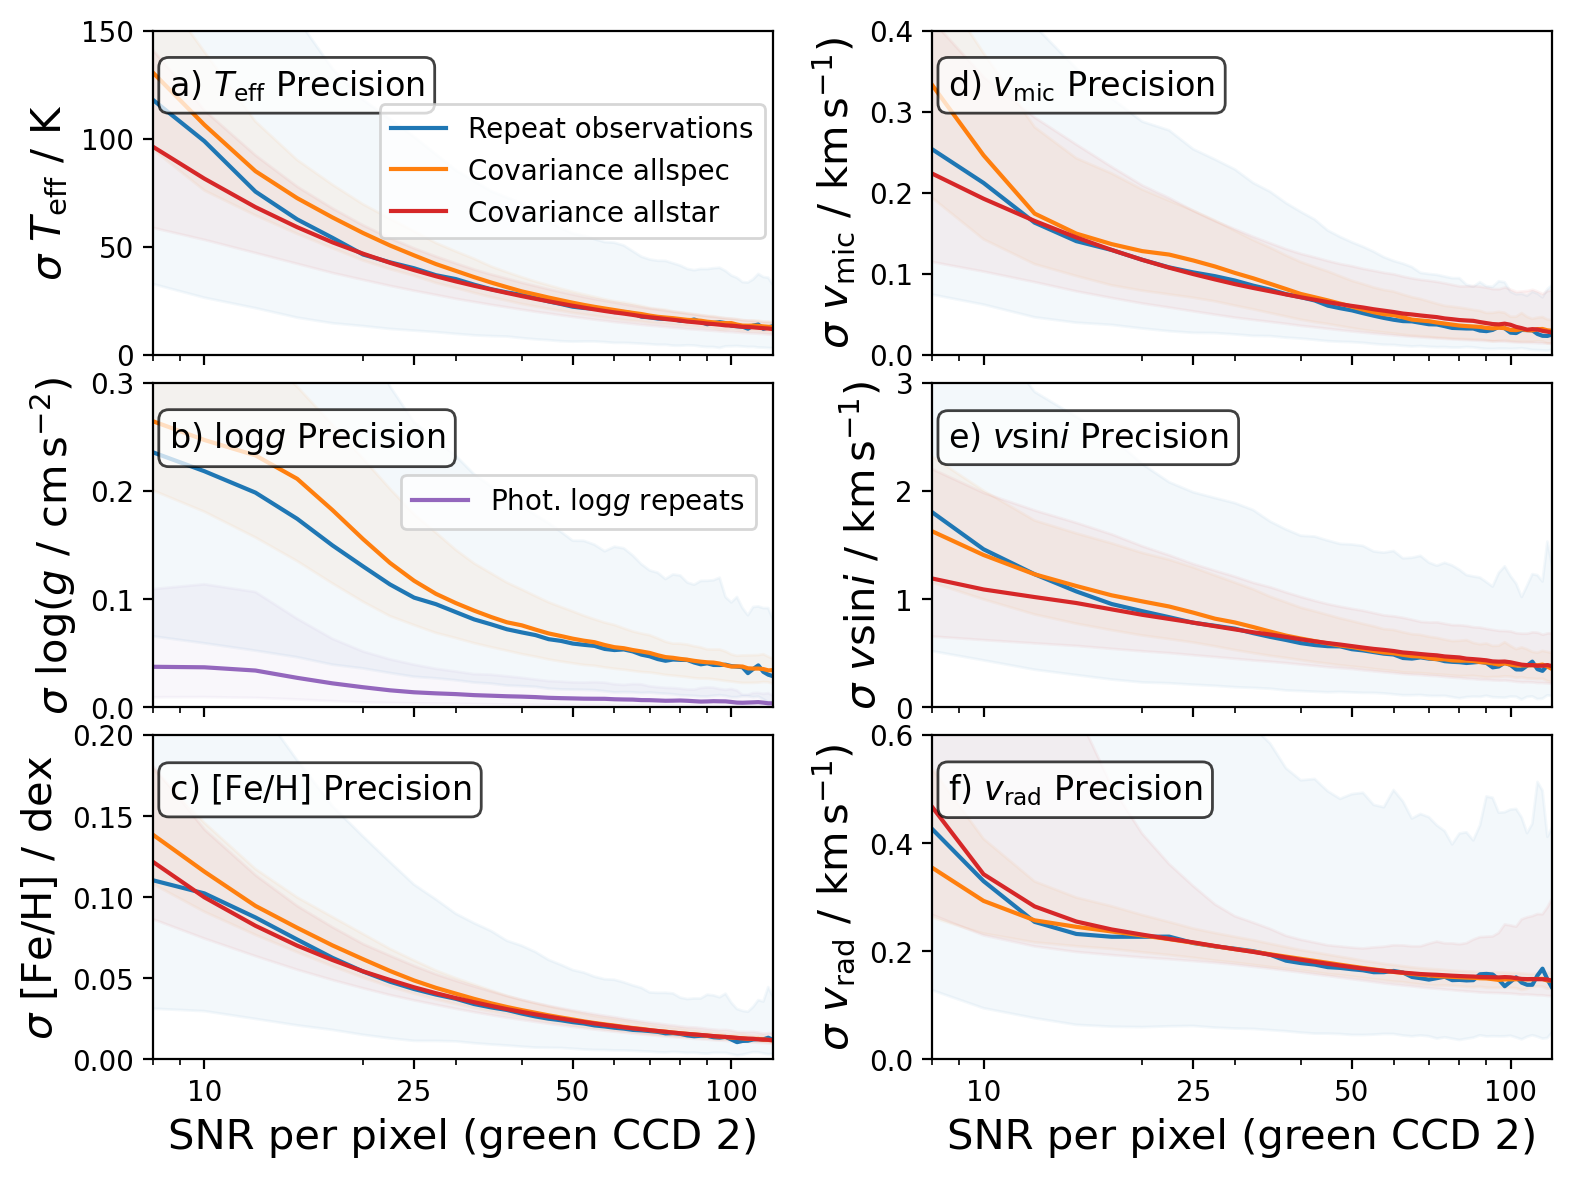
\includegraphics[width=\textwidth]{figures/galah_dr4_precision_parameters.png}
 \caption{\textbf{Precision monitoring of stellar parameters as a function of SNR for the green CCD2 across GALAH DR4.}. Each panel shows the behaviour for bins of width 10 for the scatter of repeat observations of the allspec runs (blue), covariance uncertainties of allspec (orange) and allstar (red) setups as well as scatter of photometric \logg from repeat observations (purple).}
 \label{fig:galah_dr4_precision_parameters}
\end{figure}

\subsubsection{Precision estimation and validation} \label{sec:uncertainty_precision}

In addition to the accuracy uncertainty, we estimate the total uncertainty through the additional precision uncertainty (Eq.~\ref{eq:total_uncertainty}). For this purpose, we mainly rely on the fitting uncertainties of the \texttt{curve\_fit} function, which we rescale based on repeat observations.

We note that while we report the raw fitting covariance matrix for each spectrum and module (see Fig.~\ref{fig:covariance_vesta_arcturus} for the covariance matrices of Vesta and Arcturus), their entries are not validated for reliability and have not been adjusted to incorporate a rescaling towards the final uncertainties. For the purposes of reporting stellar parameter and abundance fitting uncertainties, we restrict ourselves to the standard deviations of each feature, that is, the square root values of the diagonal covariance matrix entries.

Similar to GALAH DR3, we apply a precision adjustment of the fitting uncertainty towards consistency with the scatter of repeat observations only as a function of signal-to-noise of CCD2. Contrary to GALAH DR3, we have extended this rescaling function to be fitted in bins of signal-to-noise with both a constant, linear, and exponential term with \texttt{snr\_px\_ccd2} as the independent variable, that is, $c_1 + c2 \cdot SNR + c_3 \cdot \exp(c_4 \cdot SNR)$. We report the fitted constants for both \texttt{allspec} and \texttt{allstar} in the online repository\footnote{\texttt{*precision\_correction\_factors*} in \url{https://github.com/svenbuder/GALAH_DR4/tree/main/catalogs}.} for each stellar parameter and abundance. 

In Figs.~\ref{fig:galah_dr4_precision_parameters} and \ref{fig:galah_dr4_precision_abundances}, we then confirm that the overall trends of fitting uncertainties for \texttt{allspec} and \texttt{allstar} are consistent with the repeat observation scatter of the \texttt{allspec}. The latter has to be used as reference, because the \texttt{allstar} module uses co-added spectra of repeat observations rather than the repeat observations themselves. While this might actually overpredict the precision uncertainty of stellar parameters, we do not expect a too strong overprediction for elemental abundances.

While the precision levels of stellar parameters have on average actually remained similar to the estimates of GALAH DR3, we see notable improvement of the precision for multiple elements, such as C, Mg, V, Cr, Co, Ni, La, Ce, Nd, and Sm. We note, however, that the precision of Eu seems to have decreased.

\begin{figure}[ht]
 \centering
 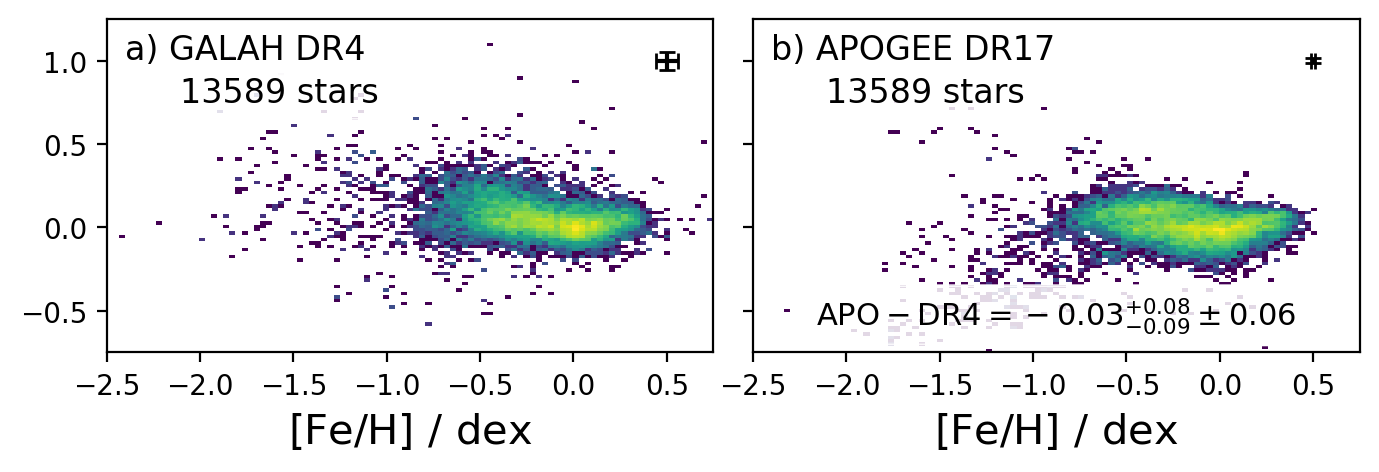
\includegraphics[width=\textwidth]{figures/comparison_dr4_apo17_C_fe.png}
 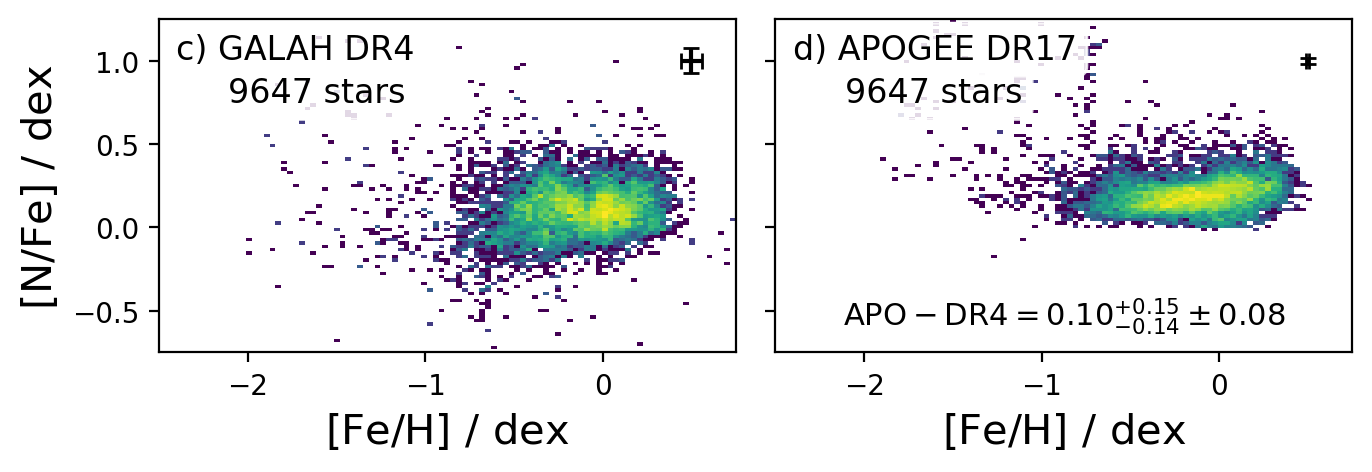
\includegraphics[width=\textwidth]{figures/comparison_dr4_apo17_N_fe.png}
 \caption{\textbf{Comparison of stars with available measurements in GALAH DR4 (left column) and APOGEE DR17 (right) for [C/Fe] (top row) and [N/Fe] (bottom row)}.}
 \label{fig:comparison_dr4_apo17}
\end{figure}

\begin{figure*}[ht]
 \centering
 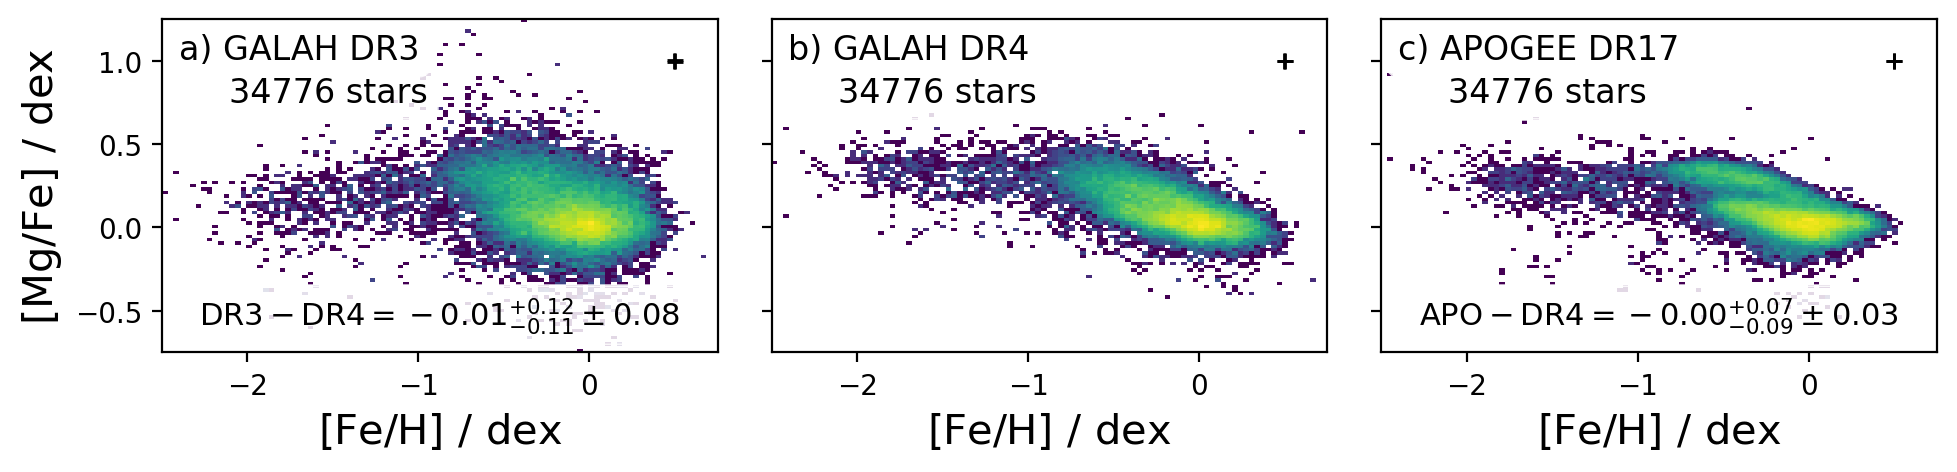
\includegraphics[width=\textwidth]{figures/comparison_dr4_dr3_apo17_Mg_fe.png}
 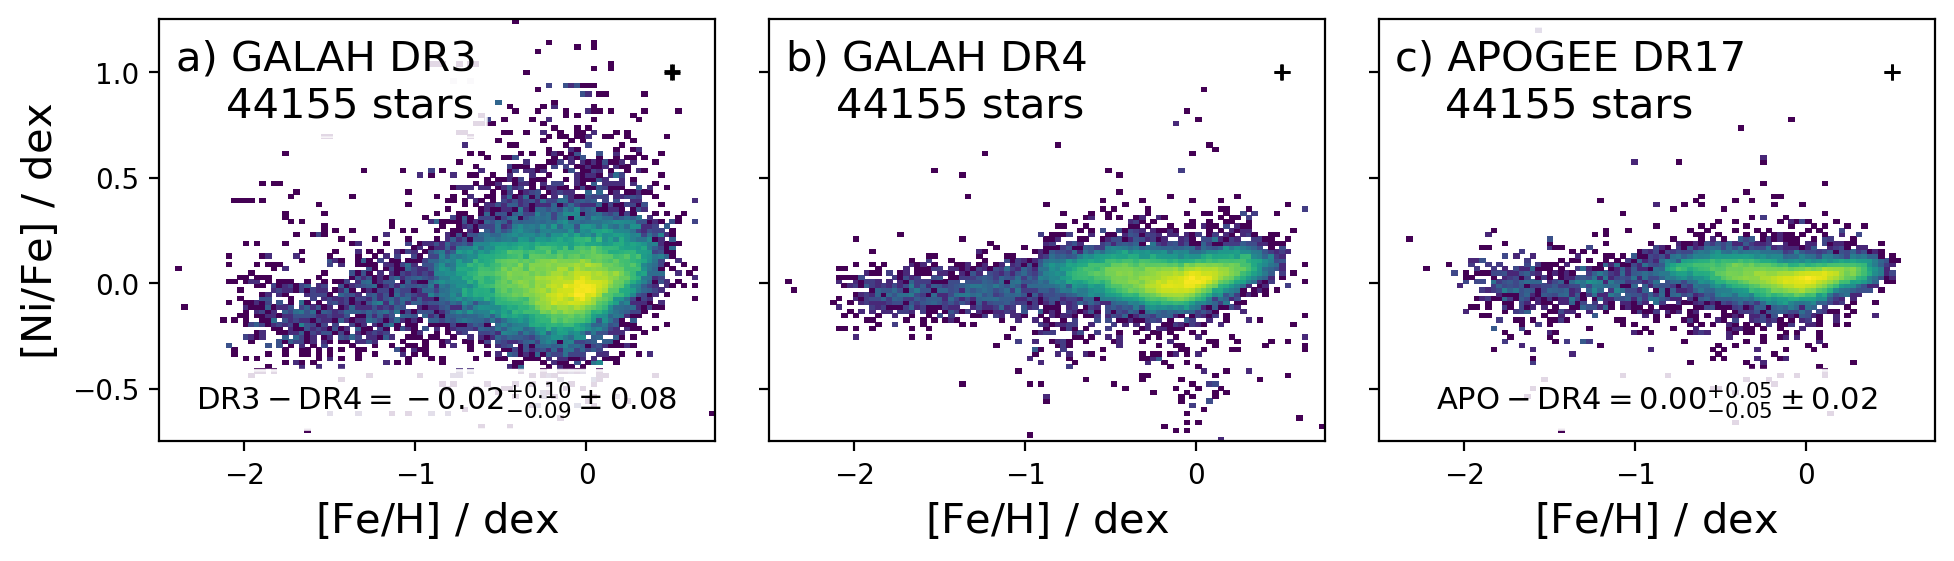
\includegraphics[width=\textwidth]{figures/comparison_dr4_dr3_apo17_Ni_fe.png}
 \caption{\textbf{Comparison of stars with available measurements in GALAH DR3 (left column), GALAH DR4 (middle) as well as APOGEE DR17 (right) for [Mg/Fe] (top row) and [Ni/Fe] (bottom row)}.}
 \label{fig:comparison_dr4_dr3_apo17}
\end{figure*}

\subsubsection{Uncertainties in light of GALAH DR3 and APOGEE DR17}

To get a better idea of the actual improvement of accuracy and precision, we have performed more elaborate comparisons as those in Fig.~\ref{fig:galah_dr4_validation_parameter_accuracy_allstar} and only showcase a few in this manuscript with reference to the online repository. We have found the comparison of GALAH DR4 with both GALAH DR3 and APOGEE DR17 highly informative.

Because GALAH DR3 did not include N measurements yet and only a limited amount of C measurements, our first comparison concerns the abundances of C and N between GALAH DR4 and APOGEE DR17 in Fig.~\ref{fig:comparison_dr4_apo17}. We attach the comparisons for the other overlapping elements O, Na, Al, Si, K, Ca, Ti, V, Cr, Mn, Co, and Ce in Figs.~\ref{fig:comparison_dr3_dr4_apo17_rest} and \ref{fig:comparison_dr3_dr4_apo17_rest2}. While we see a generally good agreement of the shapes, we notice both a bias of $-0.03\dex$ and $0.10\dex$ for C and N, respectively. These can be, however, explained with the lower precision of GALAH and might, in part, be driven by the slightly different trends of C and N towards lower metallicities. In particular, [C/Fe] decreases to sub-Solar level for APOGEE DR17 for metal-poor stars, whereas it is Solar or even enhanced in GALAH DR4. Enhanced levels would be expected for metal-poor disk stars, whereas sub-Solar levels are expected for accreted stars \citep{Amarsi2019c}, warranting a future population analysis to test the accuracy of either survey.

In addition to these novel abundances, we also showcase two previously measured abundances, namely [Mg/Fe] and [Ni/Fe] in Fig.~\ref{fig:comparison_dr4_dr3_apo17}. The $\upalpha$-process element Mg has significant value in Galactic studies because it is predominantly produced by core-collapse supernovae \citep{Kobayashi2020}. In GALAH DR3, only the \ion{Mg}{i}~$5711\,\text{\AA}$ line was used, whereas we are now using a combination of several lines. This has led to a significant improvement in precision, as can be appreciated from the comparison of Figs.~\ref{fig:comparison_dr4_dr3_apo17}a and \ref{fig:comparison_dr4_dr3_apo17}b. Even more positive, we see an improved agreement of the [Fe/H] vs. [Mg/Fe] measurements between GALAH DR4 (Fig.~\ref{fig:comparison_dr4_dr3_apo17}b) and APOGEE DR17 (Fig.~\ref{fig:comparison_dr4_dr3_apo17}c), with no abundance bias. One of the elements with the most significant precision improvement is Ni. For this element, our move to fitting the full wavelength range has increased the number of lines from two very reliable lines to several dozen lines. Albeit less reliable in their line data and possibly blended, the sheer increment in used flux information has improved the precision almost to the level of APOGEE DR17 - with no bias and a standard deviation of only $0.05\,\mathrm{dex}$ between APOGEE DR17 and GALAH DR4 (see Figs.~\ref{fig:comparison_dr4_dr3_apo17}c-f).

In addition to these instructive comparisons, we also want to return to the precision of Solar twins from Fig.~\ref{fig:galah_dr4_age_xfe_trends_solar_twins_allstar}. Here we specifically want to highlight the significant improvement of precision from GALAH DR3 to GALAH DR4 with respect to the linear estimate from \citet{Bedell2018} for C (from 0.09 to 0.045), Si (from 0.04 to 0.023), Ca (0.07 to 0.049), Ti (0.05 to 0.031), V (0.13 to 0.050), Cr (0.06 to 0.024), Ni (0.07 to 0.033), and Y (0.12 to 0.080). This improvement of sometimes a factor of 2 is remarkable and most of our comparisons indicate that these values are representative of a precision improvement beyond the Solar twins, as shown for example for Ni in Fig.~\ref{fig:comparison_dr4_dr3_apo17}.

%%%%%%%%%%%%%%%%%%%%%%%%%%%%%%%%%%%%%%%%%%%%%%%%%%%%%%%%%%%%%%%%%%%%%%%%%
\subsection{Stellar parameter flags \texttt{flag\_sp}}
\label{sec:flag_sp}
%%%%%%%%%%%%%%%%%%%%%%%%%%%%%%%%%%%%%%%%%%%%%%%%%%%%%%%%%%%%%%%%%%%%%%%%%

We have implemented a series of post-processing routines to assess the quality of the stellar parameter determinations. These routines check for a variety of potential issues with the spectra and stellar label fitting, with each flag corresponding to a specific quality check. If any of these checks are not passed, the respective bit in the quality flag \texttt{flag\_sp} is raised. The description of the implemented bits/flags for \texttt{flag\_sp} and how often they were raised is listed in Tab.~\ref{tab:flag_sp} and distributions in the Kiel diagram (\Teff and \logg) are shown for each raised bit in Fig.~\ref{fig:flag_sp_overview_allstar} for the \texttt{allstar} catalogue. For examples of stars with raised flags, we refer back to the emission line star (\texttt{flag\_sp} = 1) of Fig.~\ref{fig:examples_flag_sp_1} and the clearly double-lined binary of Fig.~\ref{fig:examples_flag_sp_2}.

Because quality cuts should be applied based on the specific science case at hand, we do not make a strict recommendation for which upper limit of \texttt{flag\_sp} should be applied. We not, however, that we have tried to implement flags that increase in concert. The first 8 bit masks (with values up to $9^2-1 = 511$) are therefore less problematic than those of 9  or higher ($\texttt{flag\_sp} \leq 512$).

\begin{table}[ht]
\centering
\caption{List of major quality flag \texttt{flag\_sp} listing the bit, description and how often the flag was raised for the \textit{allstar} and \textit{allspec} routines. Notes: Multiple bits can be raised for each of the 1\,085\,520 spectra spectra of the  of 917\,588 stars.}
\label{tab:flag_sp}
\begin{tabular}{ccccc}
\hline \hline
Raised Bit & Flag & Description & \textit{allstar} & \textit{allspec} \\
\hline
  & 0 & No flag & 700125 & 663075 \\ 
0 & 1 & Emission & 9568 & 7646 & \\
1 & 2 & CCD missing & 70078 & 44344 & \\
2 & 4 & Spectr. Binary 1 & 0 & 25538 & \\
3 & 8 & Spectr. Binary 2 & 34833 & 32566 & \\
4 & 16 & $\chi^2 > 3\sigma$ & 66859 & 20544 & \\
5 & 32 & \vsini warning & 138317 & 95990 & \\
6 & 64 & \vmic warning & 99692 & 78686 & \\
7 & 128 & Triple Binary warning & 0 & 0 & \\
8 & 256 & \Teff warning & 0 & 0 & \\
9 & 512 & \logg warning & 19863 & 10900 & \\
10 & 1024 & \feh warning & 0 & 0 & \\
11 & 2048 & S/N low & 123736 & 71154 & \\
12 & 4096 & Not converged & 32986 & 0 & \\
13 & 8192 & Model extrapolated & 69613 & 5953 & \\
14 & 16384 & No Results & 7400 & 10899 & \\
\hline
\end{tabular}
\end{table}

While not intended to identify binaries, we believe that both the \vsini and \vmic flags are informative for binaries below $T_\mathrm{eff} < 6000\,\mathrm{K}$ (see their elevated position in Figs.~\ref{fig:flag_sp_overview_allstar}f and \ref{fig:flag_sp_overview_allstar}g). We have trained the stars of this region with a lower maximum \vsini range that would be reached for a spectrum that is broadened due to binarity. This region certainly overlaps with the one of identified single-lined and double-lined binaries with \texttt{flag\_sp} = 4 and 8, respectively (see Figs.~\ref{fig:flag_sp_overview_allstar}c and \ref{fig:flag_sp_overview_allstar}d). For the latter, we notice that especially cool giants are picked up by the automatic algorithm as well. This might be either due to strong extinction biasing our analysis or due to lines in the spectrum not being modelled sufficiently and thus showing up as residual signal. While these stars are possibly flagged false-positively, we do also find a remarkable amount of true binaries, for which the \Gaia DR3 radial velocity is likely the systemic radial velocity, as it is close to the mean radial velocity of both components identified in GALAH DR4. In Fig.~\ref{fig:vrad_comparison_comp1_comp2_gaiadr3}, we visualise how one could use the radial velocities from GALAH DR4 and \Gaia DR3 to further assess the reliability of this flag.

\begin{figure*}[hbt]
\centering
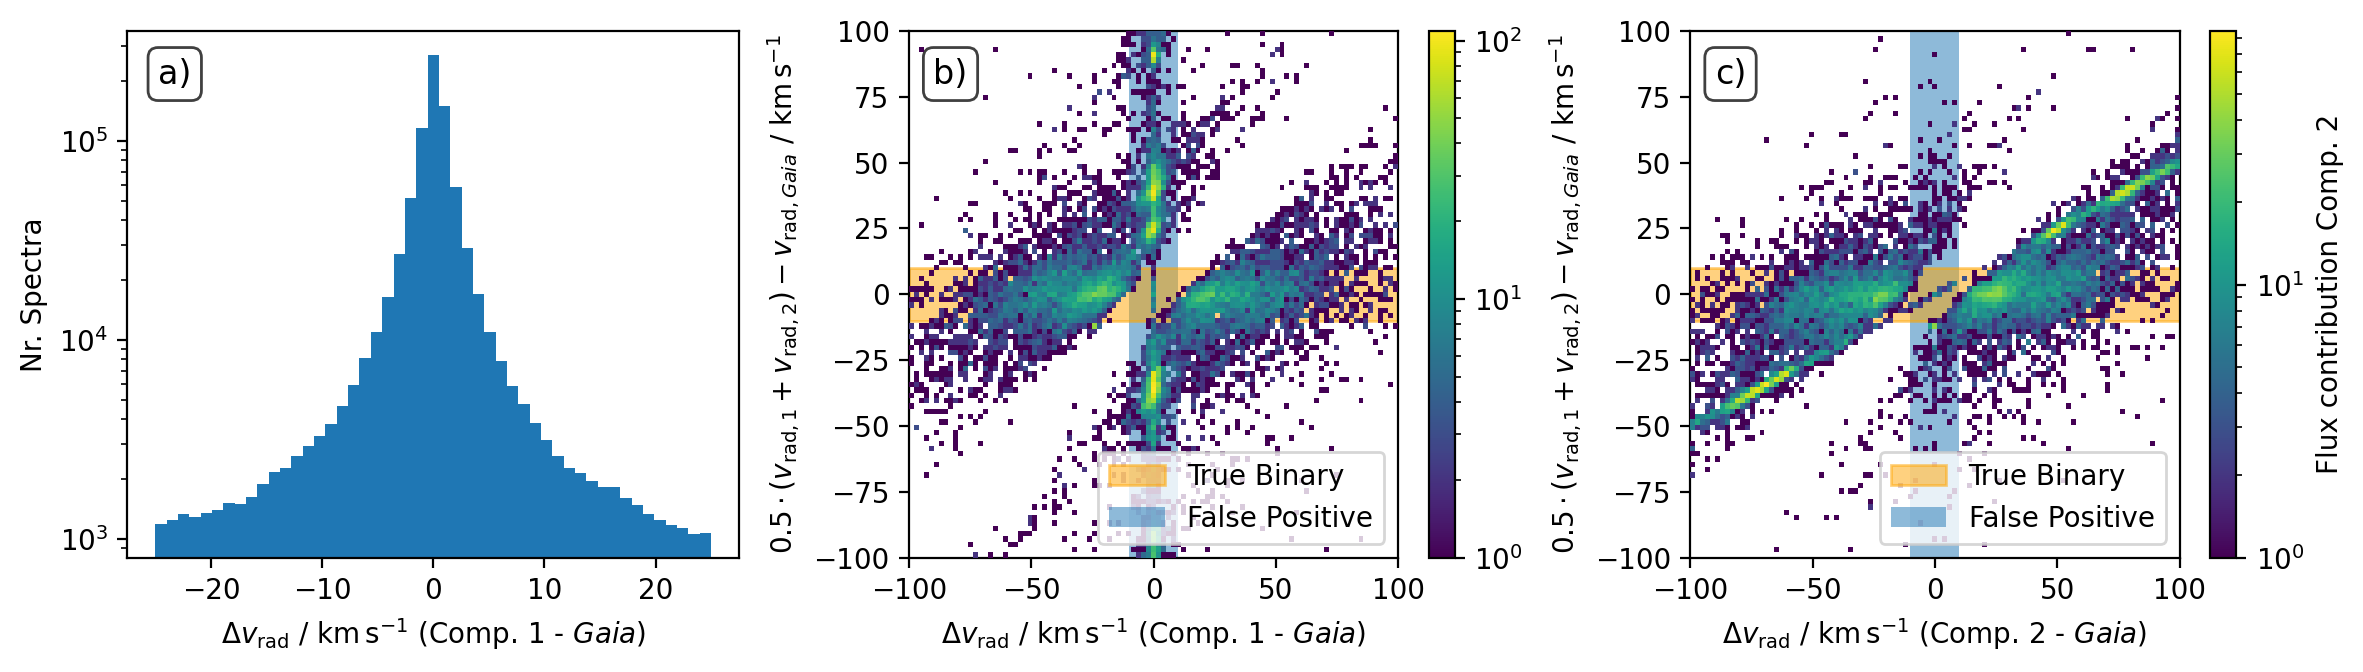
\includegraphics[width=\textwidth]{figures/vrad_comparison_comp1_comp2_gaiadr3.png}
\caption{\textbf{Comparison of radial velocity estimates of GALAH DR4 and \textit{Gaia} DR3.} \textbf{Panel a)} shows the difference of GALAH's primary component radial velocity with the mean \textit{Gaia} DR3. \textbf{Panels b) and c)} show stars for which two components were detected in GALAH DR3 and shows the difference between each component and \textit{Gaia} DR3 against the difference of mean (roughly systemic) radial velocities. The panels also include regions where actual binaries and false positive detections are expected.}
\label{fig:vrad_comparison_comp1_comp2_gaiadr3}
\end{figure*}

To check if a particular bitmask flag (e.g. $2^3 = 8$ is raised, one can perform the check in \textsc{python} via
\begin{verbatim}
    flag_8_raised = (dr4['flag_sp'] & 8) != 0
\end{verbatim}

%%%%%%%%%%%%%%%%%%%%%%%%%%%%%%%%%%%%%%%%%%%%%%%%%%%%%%%%%%%%%%%%%%%%%%%%%
\subsection{Elemental abundance flags \texttt{flag\_X\_fe}}
\label{sec:flag_x_fe}
%%%%%%%%%%%%%%%%%%%%%%%%%%%%%%%%%%%%%%%%%%%%%%%%%%%%%%%%%%%%%%%%%%%%%%%%%

The quality of elemental abundance measurements is also captured through flags. When an element is reliably detected in the spectrum, no flag is raised. However, if the abundance of an element is estimated as an upper limit, often due to weak spectral lines or low SNR, an upper limit flag is triggered. If no measurement of the element is possible, a flag is raised to indicate that the relevant spectral features were too weak or the SNR too low to allow for an estimate. The list of bits and flags for elemental abundances, \texttt{flag\_X\_fe}, is shown in Table~\ref{tab:flag_x_fe}.

By default, we recommend to only use significant detections ($\texttt{flag\_x\_fe} = 0$) for an element. Because of a bug in the flagging of the iron abundance detection (see the discussion in Sec.~\ref{sec:caveats_flags}), we do not recommend to consider $\texttt{flag\_fe\_h}$ for quality cuts.

\begin{table}
\centering
\caption{List of elemental abundance quality flags \texttt{flag\_fe\_h} for \feh or \texttt{flag\_X\_fe} for element X.}
\label{tab:flag_x_fe}
\begin{tabular}{ccc}
\hline \hline
Raised Bit & Flag & Description \\
\hline
  & 0 & detection \\ 
0 & 1 & upper limit \\ 
1 & 2 & no measurement available\\
2 & 4 & no convergence\\
3 & 8 & measurement above limit\\
4 & 16 & measurement below limit\\
5 & 32 & measurement issue of CNO \\
% problematic_cfe = (
%     # [C/N] < -1 for non-giants
%     (
%         (data['c_fe'] - data['n_fe'] < -1) & # [C/N] < -1
%         ~((data['logg'] < 3.5) & (data['teff'] < 5500)) # not_giant
%     ) |
%     # No [N/Fe] for non-giants
%     (
%         (data['flag_n_fe'] == 2) & # no [N/Fe]
%         ~((data['logg'] < 3.5) & (data['teff'] < 5500)) # not_giant
%     )
% )
%: $\mathrm{[C/N]} < -1$ for non-giants ($T_\text{eff} > 5500\,\mathrm{K}$ or $\log g > 3.5$) or no $\mathrm{[N/Fe]}$ measured for non-giants ($T_\text{eff} > 5500\,\mathrm{K}$ or $\log g > 3.5$) -> raising flag of $\mathrm{[C/Fe]}$ in that case as well as $\mathrm{[N/Fe]}$ extended non-giants ($T_\text{eff} > 5750\,\mathrm{K}$ or $\log g > 4.$ -> raising flag of $\mathrm{[N/Fe]}$ 
6 & 64 & measurement of Li, Ca, or Ba \\ %$ when CCD3 wavelength seems to be off (cdelt beyond the usual range of xx-xx) \\
\hline
\end{tabular}
\end{table}

%%%%%%%%%%%%%%%%%%%%%%%%%%%%%%%%%%%%%%%%%%%%%%%%%%%%%%%%%%%%%%%%%%%%%%%%%
\subsection{Abundance detection or upper limit}
\label{sec:abundance_detection_or_upper_limit}
%%%%%%%%%%%%%%%%%%%%%%%%%%%%%%%%%%%%%%%%%%%%%%%%%%%%%%%%%%%%%%%%%%%%%%%%%

To assess whether the abundance estimates are a true detection or an upper limit for each element X, we compare a synthetic spectrum with the best fit parameters to a synthetic spectrum with the same parameters, except for element X, for which we use the lower limit abundance of the neural network. The residuals in units of sigma between the best-fit spectrum and spectrum with the lowest possible [X/Fe] or lowered \feh then allow us to identify a detection (with maximum differences beyond 3 sigma) or upper limits, for which we raise the flag \textsc{flag\_x\_fe} by 1. We note that our initial test of overall detectability (Sec.~\ref{sec:which_labels_are_optimized}) allowed us to identify elements for which not even an upper limit was expected, raising flag \textsc{flag\_x\_fe} by 2.

%%%%%%%%%%%%%%%%%%%%%%%%%%%%%%%%%%%%%%%%%%%%%%%%%%%%%%%%%%%%%%%%%%%%%%%%%
\section{DATA RELEASE PRODUCTS}
\label{sec:catalogues_release_products}
%%%%%%%%%%%%%%%%%%%%%%%%%%%%%%%%%%%%%%%%%%%%%%%%%%%%%%%%%%%%%%%%%%%%%%%%%

GALAH DR4 encompasses a diverse range of data products. We describe the most important main catalogues in Sec.~\ref{sec:data_release_catalogues} and value-added catalogues in Sec.~\ref{sec:vacs}. We further explain the data products for each spectrum and star, that is, the reduced spectra (Sec.~\ref{sec:reduced_spectra}), \texttt{allspec} products (Sec.~\ref{sec:products_allspec}), and \texttt{allstar} products (Sec.~\ref{sec:products_allstar}).

The data products are provided directly on the AAO DataCentral website at \url{https://cloud.datacentral.org.au/teamdata/GALAH/public/GALAH_DR4/}. We further provide multiple ways to interact with the data release products, which are described in Sec.~\ref{sec:interactive}.

\subsection{Main Data Release Catalogues}
\label{sec:data_release_catalogues}

\begin{enumerate}
   \item \texttt{galah\_dr4\_allspec\_240705.fits}: analysis for each spectrum (incl. radial velocity estimation for each spectrum) based on a single spectrum
   \item \texttt{galah\_dr4\_allstar\_240705.fits}: analysis for each star based on co-added spectra of each star and using non-spectroscopic information to constrain \logg
\end{enumerate}

We present the main catalogue table schema in Table~\ref{tab:main_catalog_schema}, but refer the reader to the FITS headers of each catalogue for more detailed information.

One of our greatest achievements as part of this data release is the extraction of C and N abundances for giant stars from molecular absorption features. In Fig.~\ref{fig:cn_mass}, we show how stellar mass and [C/N] ratios are correlated in GALAH DR4, as is expected based on the pioneering work by \citet{Masseron2015} and \citet{Martig2016}. Our measurements demonstrate the potential of [C/N] abundances to better separate the core-helium burning from the red giant phase (around the blue areas of Figs.~\ref{fig:cn_mass}b and \ref{fig:cn_mass}c).

\begin{landscape}
\begin{figure}[ht]
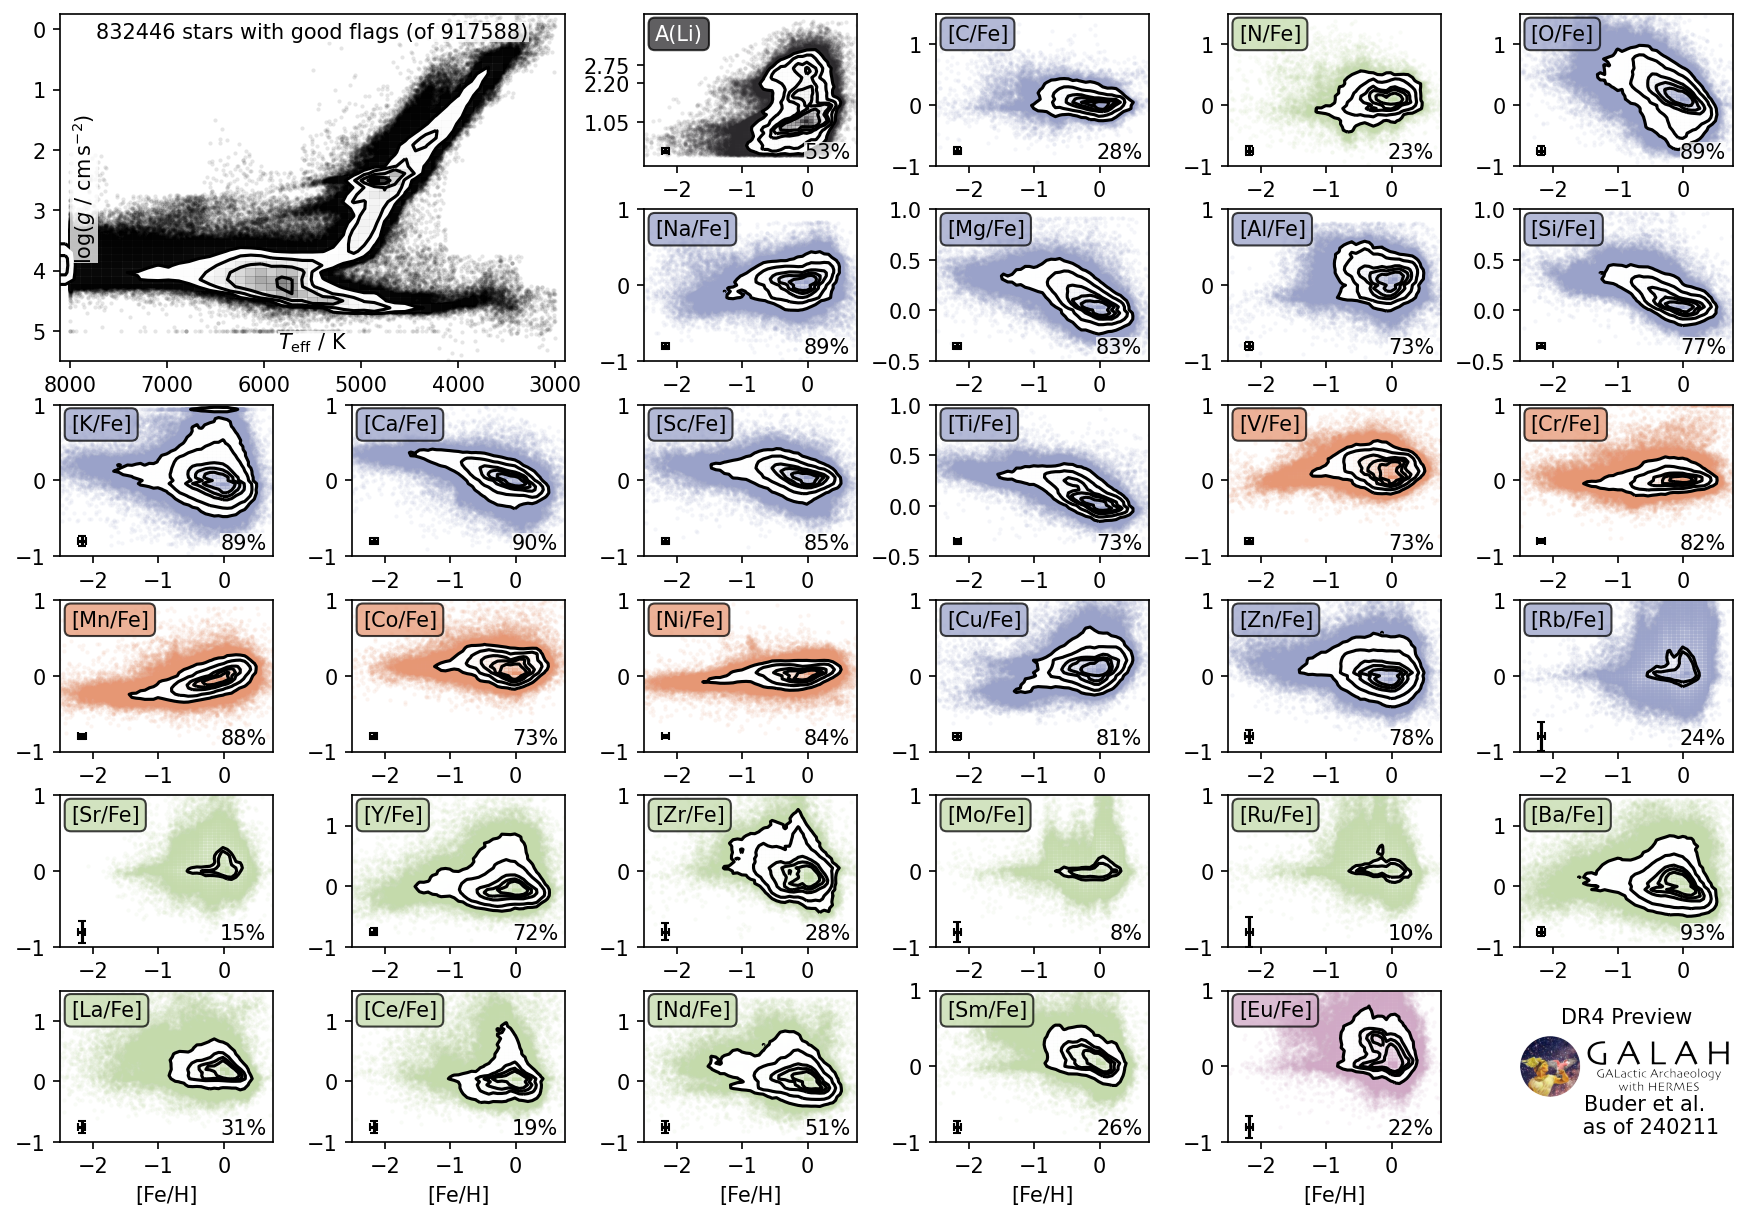
\includegraphics[width=0.975\columnwidth]{figures/galah_dr4_overview_allstar.png}
\caption{
\textbf{Overview of stellar parameters and elemental abundances for the \texttt{allstar} estimates of GALAH DR4.}
\textbf{The top left panel} shows the density distribution of stars in the Kiel diagram of \Teff and \logg.
\textbf{All other panels} show the logarithmic elemental abundances (for elements indicated in the top left of the panel) as a function of the logarithmic iron abundances \feh. Elements are colored by different nucleosynthetic channels (black for big bang nucleosynthesis, blue for core-collapse supernovae, red for supernovae type Ia, green for asymptotic giant branch star contributions and pink for the rapid neutron capture process with contributions from merging neutron stars) following the color schema from \citet{Kobayashi2020}.
}
\label{fig:galah_dr4_overview_allstar}
\end{figure}
\end{landscape}

\begin{figure*}[ht]
    \centering
    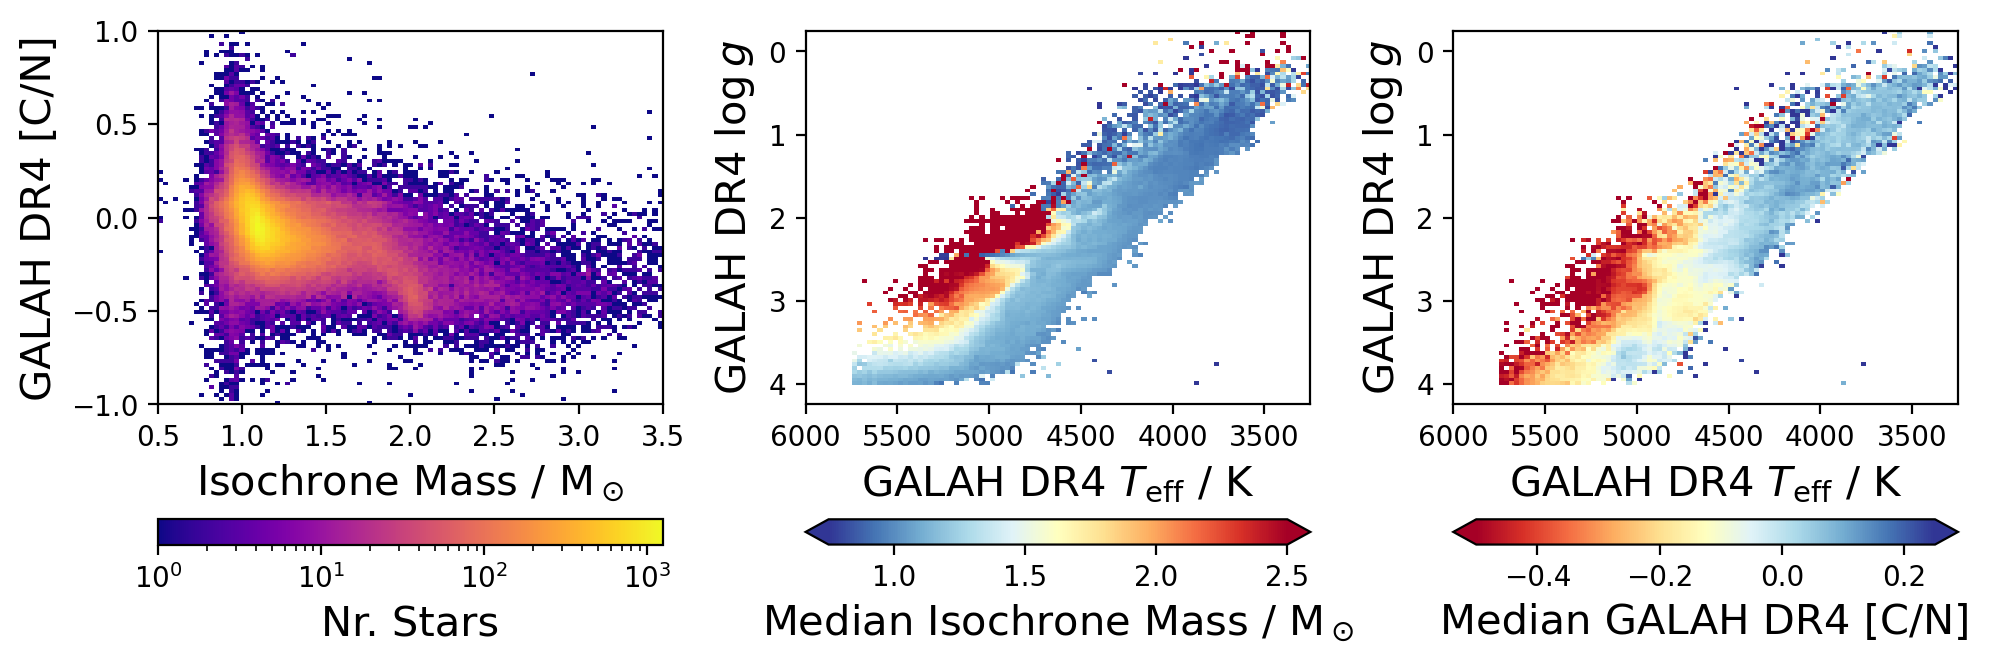
\includegraphics[width=\textwidth]{figures/cn_mass.png}
    \caption{The ratio of [C/N] and isochrone masses in comparison (panel a), and as a function of \Teff and \logg in panels b) and c), respectively}
    \label{fig:cn_mass}
\end{figure*}

\subsection{Value-Added Catalogues (VAC)} \label{sec:vacs}

We provide several value-added catalogues, namely a crossmatch catalogue to all entries of the \Gaia DR3 main source catalogue and the most important entries from the 2MASS and WISE catalogues, a catalogue of stellar dynamic properties, a catalogue of 3D NLTE measurements of Li, \SB{and a catalogue with ages inferred via isochrone interpolation in a Bayesian framework}.

\subsubsection{VAC of crossmatches with \Gaia DR3, 2MASS and WISE} \label{sec:vac_crossmatch}

The value-added catalogue of the crossmatch\footnote{\texttt{galah\_dr4\_vac\_wise\_tmass\_gaiadr3}} with the \Gaia DR3, 2MASS, and WISE catalogues as well as the distance catalogue by \citet{BailerJones2021} was calculated by performing an \texttt{OUTER JOIN} ADQL-query in the \Gaia archive. 

The query first performed an \texttt{INNER JOIN} with the 2MASS near-infrared photometry catalogue\footnote{\texttt{gaiadr1.tmass\_original\_valid}} \citep{Skrutskie2006} via its \texttt{designation} and linked this match to the \Gaia DR3 catalogue via the best neighbour\footnote{ \texttt{gaiadr3.tmass\_psc\_xsc\_best\_neighbour}} and joined\footnote{\texttt{gaiadr3.tmass\_psc\_xsc\_join}} catalogues of 2MASS to \Gaia DR3 \citep{Torra2021}. When cross-matching between Gaia DR3 and 2MASS, some stars were associated with multiple possible matches. To ensure the best match, the data was sorted by from brightest to faintest \(G\)-band magnitude, and only the brightest match for each \texttt{sobject\_id} was retained.

The crossmatch to the WISE far-infrared photometry catalogue\footnote{\texttt{gaiadr1.allwise\_original\_valid}} \citep{Cutri2013} was performed via the \Gaia DR3's best neighbour catalogue\footnote{\texttt{gaiadr3.allwise\_best\_neighbour}} \citep{Torra2021}. The match to the distance catalogue\footnote{\texttt{external.gaiaedr3\_distance}} by \citet{BailerJones2021}  via the \Gaia DR3 \texttt{source\_id}.

The catalogue also includes uncertainties in the Gaia DR3 photometric magnitudes (\(G\), \(G_{\rm BP}\), \(G_{\rm RP}\)) that were recalculated following the recommendations from the Gaia Early Data Release 3 (EDR3) documentation \citep{Riello2021}. The total uncertainties were computed by combining the photon flux error with an additional systematic term.

We further corrected the \Gaia DR3 parallaxes for systematic zeropoint errors by applying the correction model provided by \citet{Lindegren2021b}. This correction depends on several factors, including the \(G\)-band magnitude, effective wavenumber (\(\nu_{\rm eff}\)) used in astrometry, pseudocolour, latitude, and the astrometric solution type. The parallax zeropoints and original parallaxes are reported as \texttt{plx\_zpt\_corr} and \texttt{parallax\_raw}.

In addition to the crossmatch with the \Gaia DR3 \texttt{gaia\_source} catalogue, multiple other crossmatches can easily performed via the \texttt{gaiadr3\_source\_id} column. We have for excample crossmatched the sources from GALAH DR4 with those from \Gaia DR3's variability catalogues \citep{Rimoldini2023}. We find 47\,493 stars in GALAH DR4 that are overlapping with the \textit{gaiadr3.vari\_classifier\_result} catalogue. In particular, we find 17\,256 SOLAR\_LIKE variables, 14\,477 stars in the DSCT/GDOR/SXPHE category ({$\updelta$}Scuti, {$\upgamma$} Doradus, or SXPhoenicis), 6\,247 LPV (long-period variables), 4\,074 ECL (eclipsing binaries), 3\,355 RS (RS Canum Venaticorum variables), 1\,096 YSO (young stellar objects), 401 RR (RR Lyrae types), and a large variety of other variables, including the white dwarf 2MASS J05005185-0930549 that was already found in GALAH data by \citet{Kawka2020}.

\subsubsection{VAC of stellar dynamics}
\label{sec:vac_dynamics}

The value-added catalogue for stellar dynamics\footnote{\texttt{galah\_dr4\_vac\_dynamics}} includes the kinematic and dynamical properties for stars in the GALAH DR4 survey. The catalogue is created with a publicly available script\footnote{Accessible in the GALAH DR4 repository \href{https://github.com/svenbuder/GALAH_DR4/blob/main/catalogs/create_galah_dr4_vac_dynamics.ipynb}{here}.} as part of GALAH DR4. 
We define the position of the Sun in our Galactic reference frame as $R_\mathrm{GC} = 8.21\,\mathrm{kpc}$ \citep{McMillan2017}, $\varphi_\mathrm{GC} = 0\,\mathrm{rad}$, and $z_\mathrm{GC} = 25\,\mathrm{pc}$ \citep{BlandHawthorn_Gerhard2016}. We then combine the total velocity in $V$ of the Sun at $R_\mathrm{GC}$ based on the proper motion measurement of $6.379\pm0.024\,\mathrm{mas\,yr^{-1}}$ by \citep{Reid2004}, that is, $V_\odot = 248.27\,\mathrm{km\,s^{-1}}$ with the circular velocity of $V_\mathrm{circ} = 233.10\,\mathrm{km\,s^{-1}}$ by \citet{McMillan2017} to estimate a peculiar velocity of the Sun with respect to the local standard of rest of  $15.17\,\mathrm{km\,s^{-1}}$. For the other two components, we use the estimate by \citet{Schoenrich2010}, leading to a peculiar velocity of the sun of $(U,V,W) = (11.1, 15.17, 7.25)\,\mathrm{km\,s^{-1}}$.

Starting from the crossmatch of GALAH DR4 with the \Gaia DR3 (see Sec.~\ref{sec:vac_crossmatch}), we use the \textsc{galpy.orbit} module by \citet{Bovy2015} to estimate heliocentric Cartesian coordinates $(X,Y,Z)$ and velocities $(U,V,W)$ as well as Galactocentric Cylindrical coordinates $(R, \varphi, Z)$ and velocities ($v_R, v_\varphi, v_Z$). We approximate the orbit actions $J_R, J_\varphi = L_Z, J_Z$ and frequencies $\omega_i$ with the \textsc{galpy.actionAngle.actionAngleStaeckel} function with a focal length of the confocal coordinate system $\texttt{delta} = 0.45$ in the Milky Way potential by \citet{McMillan2017}. We further use the Staeckel approximation \citep{Binney2012} to calculate eccentricity, maximum orbit Galactocentric height, and apocentre/pericentre radii with \textsc{galpy}'s \textsc{EccZmaxRperiRap} \citep{Mackereth2018}. Our assumption of a time-invariant, axisymmetric potential further allows us to extract the orbit energy via \textsc{galpy.Orbit.E}.

In particular the dedicated observing programs of GALAH towards low angular momentum stars (PI S. Buder) and globular clusters (PI M. McKenzie and PI M. Howell) have increased the number of spectroscopic observations for stars on halo-like orbits. This is showcased by both the action-action diagram of angular momentum $L_Z$ versus radial action $\sqrt{J_R}$ (Fig.~\ref{fig:galah_dr4_lz_jr_with_gcs}) and angular momentum $L_Z$ versus orbit energy $E$ (Fig.~\ref{fig:galah_dr4_lz_e_with_gcs}) and visualises the potential of GALAH DR4 observations to complement Galactic dynamics studies and enable Galactic chemodynamic studies.

\begin{figure}[ht]
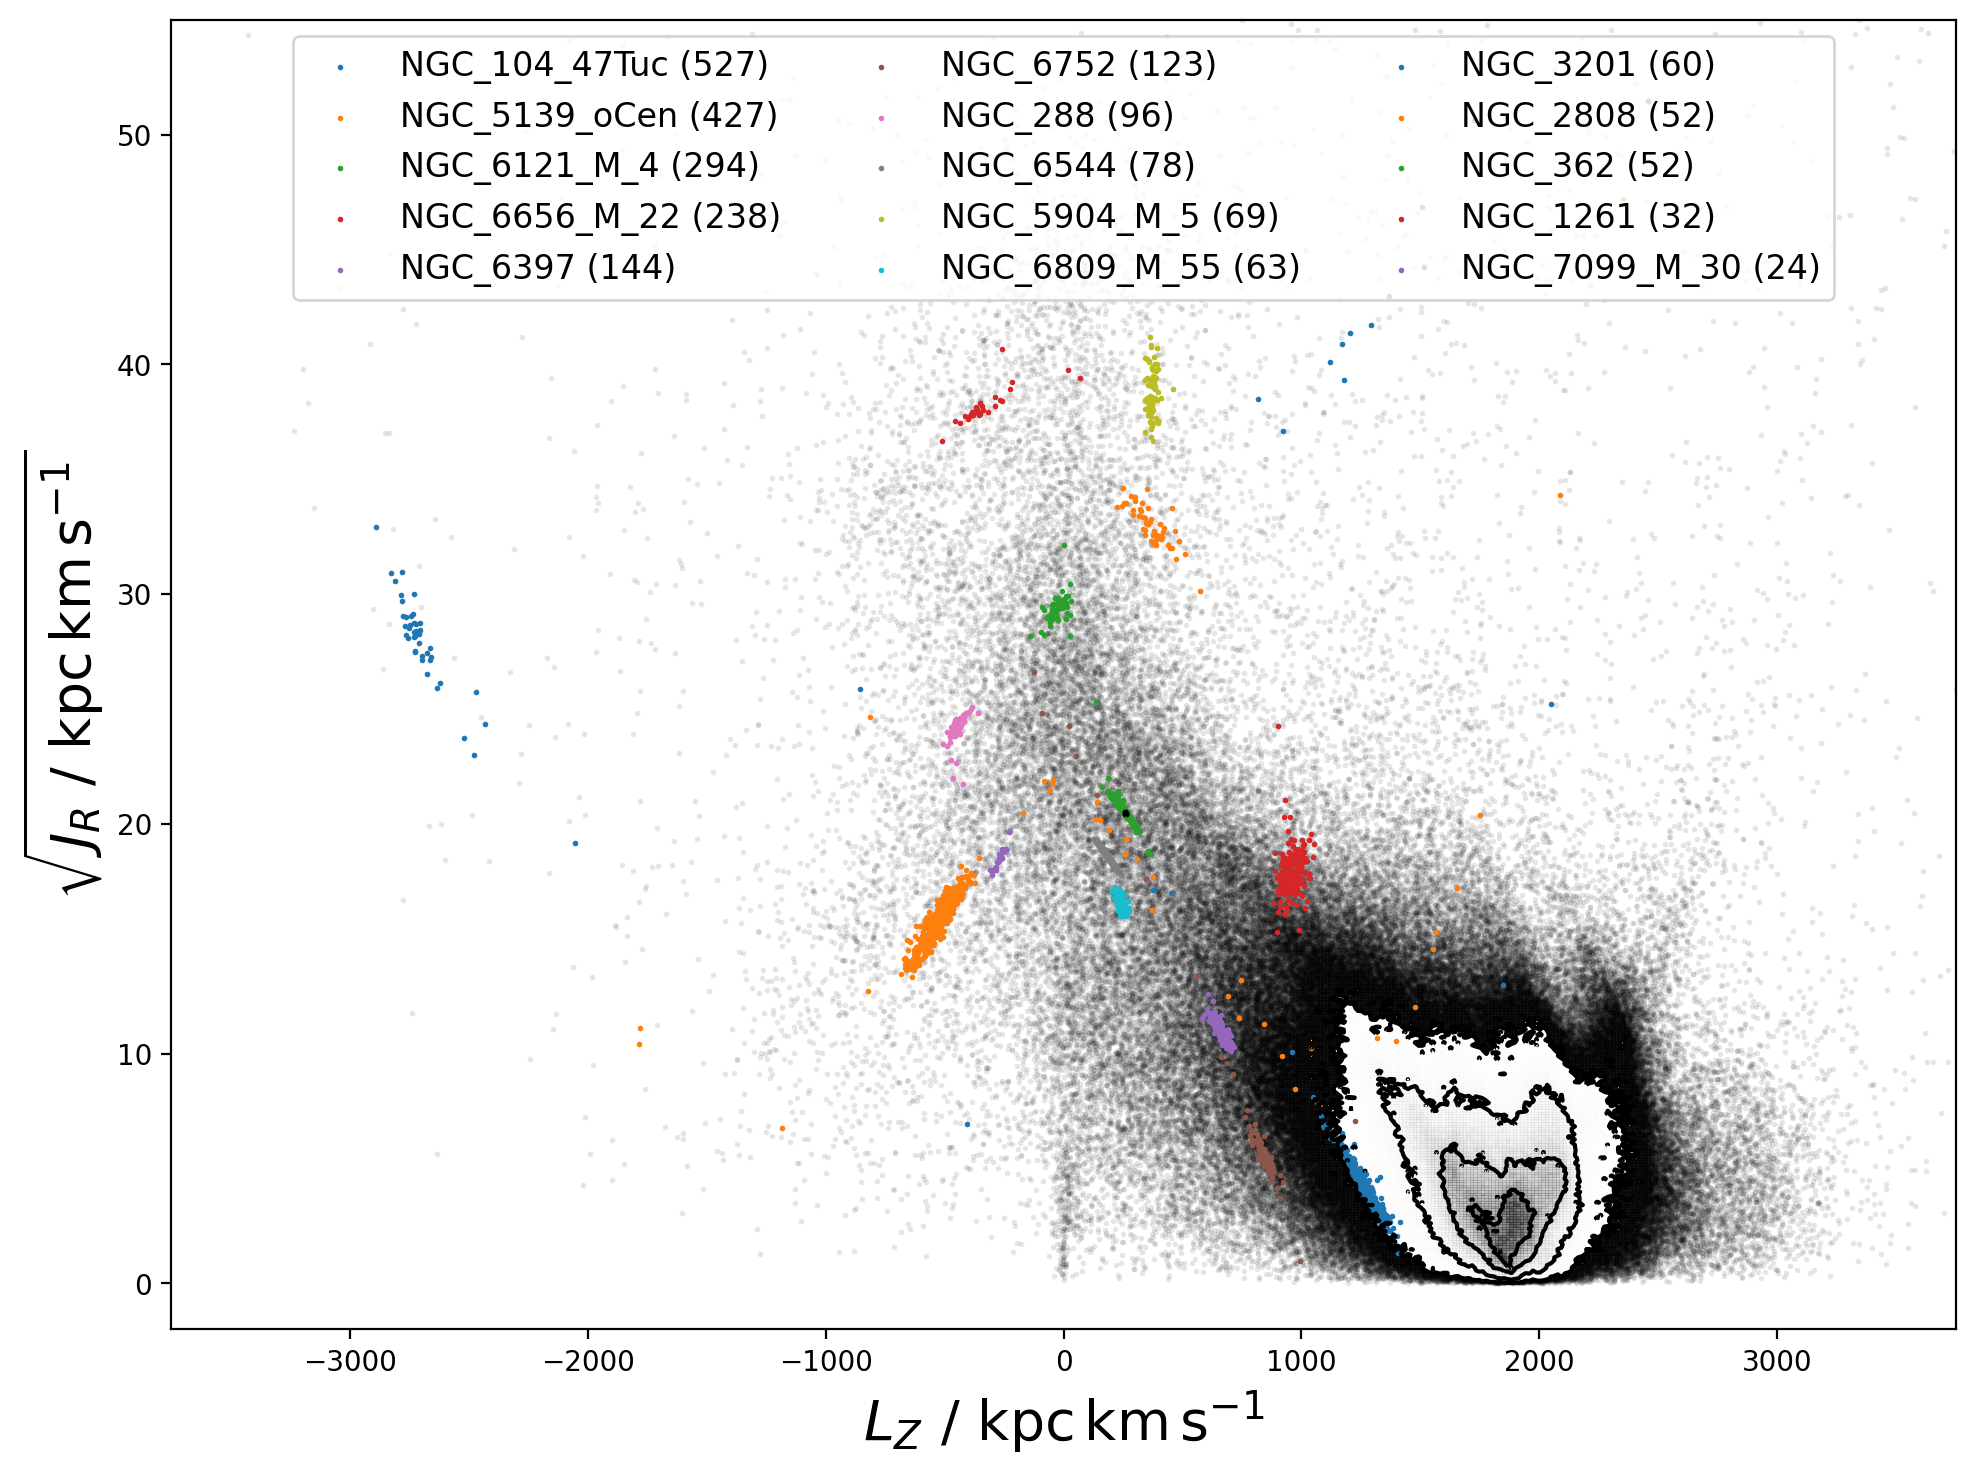
\includegraphics[width=\columnwidth]{figures/galah_dr4_lz_jr_with_gcs.png}
\caption{
\textbf{Distribution of the dynamic properties of angular momentum $L_Z$ and radial action $J_R$ of stars in GALAH DR4 (black), with globular cluster members highlighted in colour.} Cluster members were selected as those with more than 70 percent membership probability according to \citet{Vasiliev2021}. The Sun is indicated with a red $\odot$ symbol.
}
\label{fig:galah_dr4_lz_jr_with_gcs}
\end{figure}

\begin{figure}[ht]
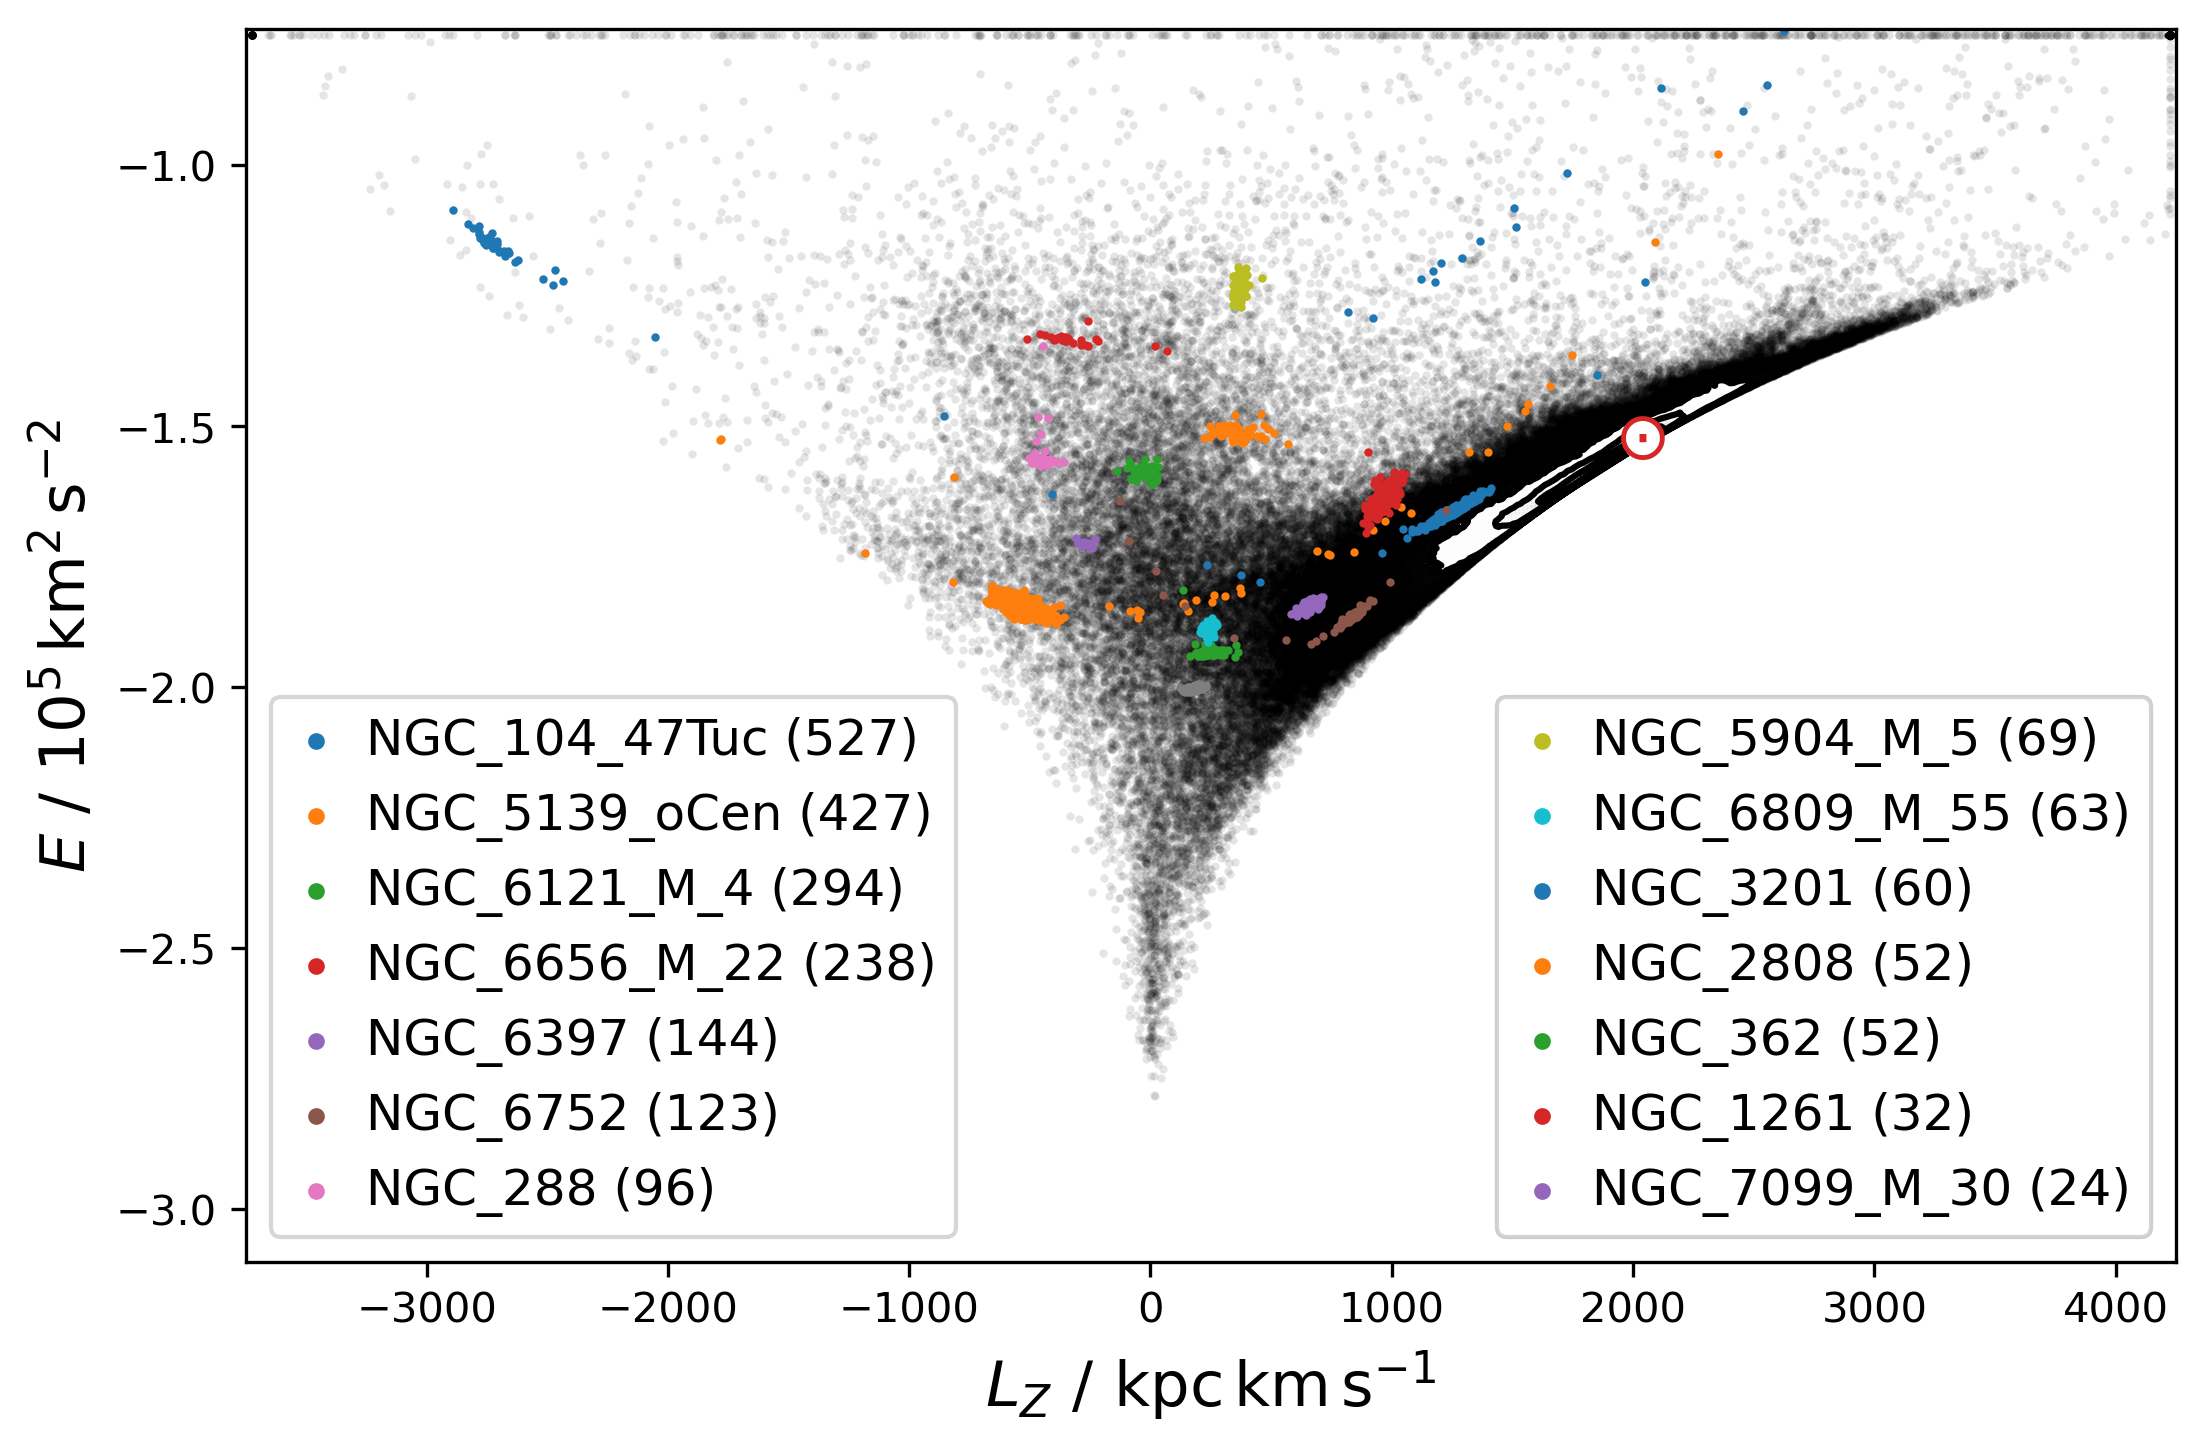
\includegraphics[width=\columnwidth]{figures/galah_dr4_lz_e_with_gcs.png}
\caption{
\textbf{Distribution of the dynamic properties of angular momentum $L_Z$ and orbit energy $E$ of stars in GALAH DR4 (black), with globular cluster members highlighted in colour.} Cluster members were selected as those with more than 70 percent membership probability according to \citet{Vasiliev2021}. The Sun is indicated with a red $\odot$ symbol.
}
\label{fig:galah_dr4_lz_e_with_gcs}
\end{figure}

\subsubsection{VAC of 3D NLTE lithium abundances}

In this value-added catalogue\footnote{\texttt{galah\_dr4\_vac\_3dnlte\_a\_li}}, we use spectrum fitting to infer 3D non-local thermodynamic equilibrium (NLTE) lithium abundances. For each spectra, the Li line is modelled with a 3D NLTE \breidablik line profile. In cases where the Li line is blended with nearby lines such as Fe and CN, we model blending lines as Gaussian absorption profiles. From this model, we measure the equivalent width (EW) and errors in EW of the Li line using \textsc{UltraNest} \citep{Buchner2021}, a Monte Carlo nested sampling algorithm. The Li abundance, A(Li), is then inferred from the measured EW using \breidablik and the stellar parameters from GALAH DR4's \texttt{allstar}. See \citet{Wang2024} for a detailed description of the methodology. 

We update this methodology to provide better performance and fitting constraints. 
\citet{Wang2024} measured a local line width for blending lines in the Li region which incorporated the thermal broadening, rotational broadening, and instrumental profile. For this work, we use the GALAH instrumental profile convolved with the GALAH rotational velocity for the line width. For the Li line, \citet{Wang2024} fitted a separate line width which includes only the rotational broadening and instrumental profile as the 3D NLTE Li line profiles are already thermally broadened. For this work, we calculate a broadening kernel based on the GALAH instrumental profile and rotational velocity and apply this kernel to the Li line. 
%\citet{Wang2024} measured a local line width for the Li region and fit the width of the Li line separately from other lines. For this work, we use the GALAH instrumental profile convolved with the rotational velocity as the width of our blending lines and set the width of the Li line based on this convolved kernel, better constraining the line widths. 
Whilst we still measure a local radial velocity due to imperfections of the wavelength solution in CCD3, we apply the GALAH radial velocity for poorly constrained Li depleted stars where we cannot measure the local radial velocity. In addition, the sampled EW posterior is now modelled using a first order boundary corrected kernel density estimator from \citet{Lewis2019}, which has better convergence than histograms. Lastly, GALAH DR4 analyses stars down to 3000\,K, but the \stagger model atmospheres only reach 4000\,K, therefore, we provide an additional column of 1D NLTE A(Li) inferred through our EWs using \breidablik on \marcs model atmospheres. 
%Note that these 1D NLTE Li abundances are different from the 1D NLTE Li abundances published in \texttt{allstar}.
Using the updated methodology it takes $\sim$2 minutes per star in comparison to $0.5$--$2$ hours per star reported in \citet{Wang2024}, with the main speed up coming from fixing the Li line width. 

%apply a methodology described in \citet{Wang2024}, leveraging GALAH DR4's \texttt{allstar} spectra and parameters to derive equivalent width (EW) measurements and infer 3D non-local thermodynamic equilibrium (NLTE) lithium abundances, A(Li). The lithium line profiles are blended with nearby lines, such as Fe and CN, which are modeled with a combination of Gaussian absorption lines. The equivalent width of the blended Li feature is measured using a Monte Carlo nested sampling algorithm, which explores the posterior distribution of the parameters and generates multiple realizations of the spectra.

%The abundance of A(Li) is then inferred by interpolation of the EW to A(Li) relation from a pre-calculated grid. 

EWs are measured for 892\,223 stars (97\% of GALAH DR4), with 3D NLTE A(Li) detections reported for 417\,825 stars (46\%) and upper limits for 474\,398 stars (52\%). Fig.~\ref{fig:mean_ew} shows the mean EW over \Teff and \logg. The Li-dip can be seen on the main sequence turn-off at \Teff$\approx 6500$\,K and \logg$\approx 4.2$ and extends up the subgiant branch. There is a Li enhanced population of stars at \logg$\approx 2.5$ in the red clump whilst the horizontal branch is depleted in Li. The increase of mean Li EW up the giant branch is due to a large proportion of stars with EW$\approx 100$\,m\AA. Features of this figure will be studied in followup papers. 
A quality flag (\texttt{flag\_ALi}) is raised by 1 for upper limits, 2 or more to indicate other quality issues, such as stellar parameters falling outside of the model atmosphere grid (see \citet{Wang2024} for more details on the bitmask flag). We recommend \texttt{flag\_ALi < 2} when using the 3D NLTE A(Li), and \texttt{flag\_ALi < 4} when using Li EWs. A similar quality flag \texttt{flag\_ALi\_1D} is provided corresponding to the 1D NLTE A(Li) included in the VAC. 
% This detailed process ensures the catalogue provides high-precision lithium measurements, advancing our understanding of lithium production and depletion mechanisms throughout stellar evolution.

\begin{figure}[ht]
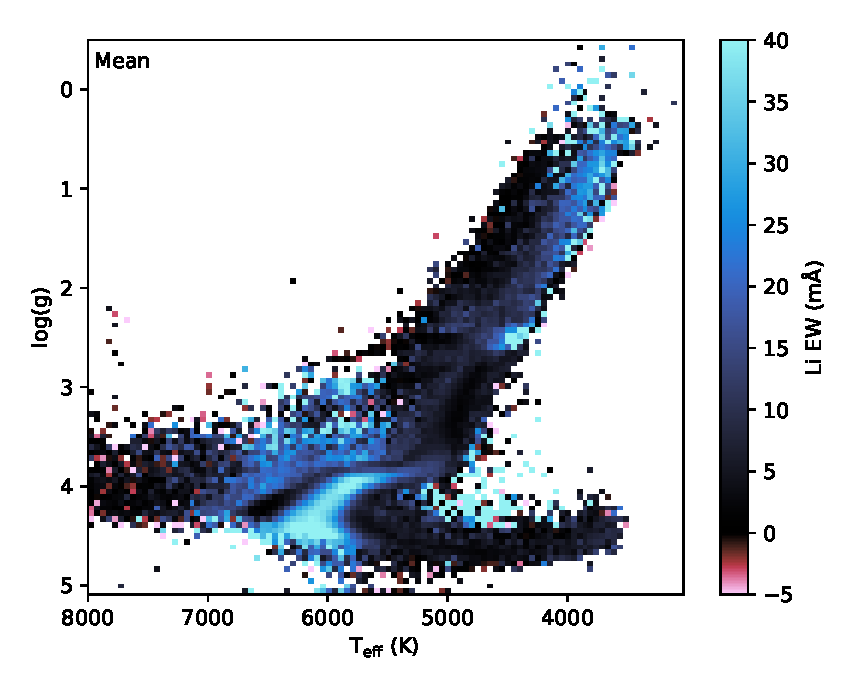
\includegraphics[width=\columnwidth]{figures/mean_ew.eps}
\caption{
Mean EW binned in \Teff and \logg. The Li-dip can be seen at \Teff$\approx 6500$\,K and \logg$\approx 4.2$. At \logg$\approx 2.5$, red clump stars have a higher mean Li EW whilst horizontal branch stars have a lower mean Li EW compared to surrounding stars. The mean Li EW increases going up the red giant branch. 
}
\label{fig:mean_ew}
\end{figure}

For convenience, we have included the most important columns of this catalogue in the \texttt{allstar} catalogue (see Table~\ref{tab:main_catalog_schema}), as we recommend to use them instead of the less accurate 1D NLTE abundances estimated with an imperfect neural network interpolation, which we indicate with \texttt{nn\_li*}.

\subsubsection{Ages}

\SB{TBD.}

\subsection{Data products for each spectrum and star}
\label{sec:data_products_for_each_spectrum}

We provide individual data products in an orderly fashion that allow users to create links to these products based solely on the \texttt{sobject\_id}. To download data products for individual stars we recommend creating a url string and using \textsc{wget} or similar commands. For bulk downloads of the advanced data products of this section, we recommend contacting the GALAH collaboration or using the bulk download interfaces of AAO DataCentral.

\subsubsection{Reduced spectra} \label{sec:reduced_spectra}

The reduced spectra of each night are provided in the observations directory\footnote{\texttt{observations/YYMMDD/spectra/com/sobject\_id*.fits}} and sorted into directories with four spectra - one for each of the four CCDs. These spectra are produced by the reduction pipeline (see Sec.~\ref{sec:spectroscopic_data_from_galah_observations}) and include several extensions as outlined in Table~\ref{tab:reduction_fits}, with wavelength information stored in the fits headers with starting wavelength \texttt{CRVAL1} in \AA and linear pixel scale \texttt{CDELT1} in \AA/px, and the number of pixels \texttt{NAXIS1}. The reduced spectra are only provided per exposure and not in a co-added manner, since the co-adding was performed as part of the \texttt{allstar} module (see Sec.~\ref{sec:products_allstar} for co-added spectra). We note that not all files might be available for a given exposure due to the seldom failure of CCD readouts.

\subsubsection{Additional products of the \texttt{allspec} module} \label{sec:products_allspec}

The \texttt{allspec} analysis product directory\footnote{\texttt{analysis\_products\_single/YYMMDD/sobject\_id/}} provides the files that were produced by the \texttt{allspec} module. These include the on-the-fly assessment of the radial velocity fit \texttt{*rv.png} (similar Fig.~\ref{fig:181221003101356_single_fit_rv}), the raw fitting results \texttt{*results.fits} and their covariance matrices \texttt{*covariances.npz} (similar to the entries used to produce Fig.~\ref{fig:covariance_vesta_arcturus}). We also provide a combined \texttt{*spectrum.fits} file (concatenated over the four bands) that includes the wavelength, flux, and flux uncertainty of the velocity-corrected and re-normalised observed spectrum as well as the best-fit model spectrum interpolated onto the same wavelength. Finally, we provide an \texttt{*comparison.pdf} (similar to Fig.~\ref{fig:210115002201239_allstar_fit_comparison}) which displays the fit results, comparison of observed and model spectrum, masked wavelength regions, and wavelengths of the most important element lines. If the module did not run to completion, for example because the SNR of the spectra was below the threshold of $\mathrm{SNR} > 10$ for any CCD to even attempt a fit, not all products are available for a spectrum.

\subsubsection{Additional products of the \texttt{allstar} module} \label{sec:products_allstar}

The \texttt{allstar} analysis product directory\footnote{\texttt{analysis\_products\_allstar/YYMMDD/sobject\_id/}} also include the radial velocity monitoring \texttt{*rv.png}, results files  \texttt{*results.fits}, combined spectra \texttt{*spectrum.fits} and \texttt{*comparison.pdf} overview, similar to the ones described in Sec.~\ref{sec:products_allspec}. In addition, each directory also includes a \texttt{*sobject\_ids.txt} file that lists all individual spectra that were co-added to create the observed spectrum and its uncertainty in \texttt{*spectrum.fits}.

% TBD: For easier downloading, we also provide these files in tar-files per night. Furthermore, we have interpolated all normalised allstar spectra onto a common wavelength that includes the largest possible wavelength coverage of 99.9\% of radial velocity corrected spectra (neglecting pixels below 7680\AA for the infrared channel).

\subsection{Interactive access via AAO DataCentral}
\label{sec:interactive}

In collaboration with the AAO Data Central, a number of interactive ways are provided to explore the data of this release. Data Central provides both Simple Spectral Access and Single Object Viewer services. In addition, we recommend to download files or easily crossmatch user catalogues with the TAP server \url{https://datacentral.org.au/vo/tap} in TOPCAT \citep{Taylor2005}. \url{https://apps.datacentral.org.au/galah/spectra} also provides An interactive plotting application to show normalised or un-normalised spectra of different repeat observations. As these tools are under active development, we refer to the latest documentation on both the DataCentral and the main Survey website \url{https://www.galah-survey.org}.

\section{CAVEATS AND FUTURE IMPROVEMENTS} \label{sec:caveats}

In this section, we attempt a detailed discussion of caveats along different steps of our analysis, while also giving suggestions for future improvements - both for GALAH and other surveys. We first discuss caveats of the spectrum reduction (Section~\ref{sec:caveats_reduction}), before extensively discussing the spectrum synthesis (Section~\ref{sec:caveats_synthesis}) and spectrum interpolation (Section~\ref{sec:caveats_interpolation}). We discuss possible problems arising from the use of photometric information (Section~\ref{sec:caveats_photospec}), in particular for stars that could be binaries (Section~\ref{sec:caveats_binaries}). While we have attempted to already flag possible caveats, we also lay out problematic flags in (Section~\ref{sec:caveats_flags}). We summarise the most important caveats in Section~\ref{sec:caveats_summary}.

\subsection{Spectrum reduction}  \label{sec:caveats_reduction}

Although a significant amount of work was spent on improving the spectrum reduction, we want to lay out a few areas that could still suffer from imperfection.

\subsubsection{Wavelength solutions}

For each CCD, the reduction pipeline estimates the most suitable wavelength solution, linking pixels with actual wavelengths based on the ThXe arc lines. In GALAH DR3 \citep{Buder2021} we identified several issues for spectra where not enough ThXe lines could be used to constrain the wavelength solution. Improvements have been made for the new reduction version to improve the number of useful ThXe lines and restrict the flexibility of wavelength solutions to move them closer to previous results. This has helped us to decrease the amount of problematic wavelength solutions towards the end of CCD3, with the only used absorption lines of Li and Eu, from an initially bad wavelength solution for 7.9\% of the spectra.

\subsubsection{Holistic spectrum extraction}

Although much work has been spent on improving telluric and sky lines in the reduction step, most reduction steps are currently run sequentially rather than in parallel. Using the information of stellar spectra when modelling the wavelength solution would certainly help to overcome the limited information in ThXe calibration spectra in the absence of laser combs \citep{Kos2018b}. Multiple steps in this direction have been taken \citep{Saydjari2023} and should be rolled out in future spectrum analysis. This would especially help to mitigate imperfect telluric and sky line removal while simultaneously improving the wavelength solution -- among many other effects.

\subsection{Imperfect spectrum synthesis} \label{sec:caveats_synthesis}

\subsubsection{Spectrum synthesis}

The GALAH survey's success relies heavily on the ability to accurately model stellar spectra to infer accurate stellar properties. The survey has seen significant improvements in moving from the approximation of 1-dimensional (1D) atmospheres with local thermodynamic equilibrium (LTE) towards 1D NLTE, that is, statistical (or non-local) thermodynamic equilibrium \citep{Amarsi2020}. This includes the use of 1D NLTE synthesis for atomic lines  H \citep{Amarsi2018}, Li \citep{Lind2009, Wang2020}, C \citep{Amarsi2019}, N \citep{Amarsi2020b}, O \citep{Amarsi2018b}, Na \citep{Lind2011}, Mg \citep{Osorio2015}, Al \citep{Nordlander2017}, Si \citep{Amarsi2017}, K \citep{Reggiani2019}, Ca \citep{Osorio2019}, Mn \citep{Bergemann2019b}, Fe \citep{Amarsi2018, Amarsi2022}, and Ba \citep{Gallagher2020} for the {\sc marcs} model atmosphere grid. The work by \citet{Wang2024} also enables us to present measurements of Li in 3D NLTE as part of this release.

All of these advances contrast with the lack of a proper way of modelling molecular features appropriately. This could explain the significant mismatch of oxygen abundances between optical and infrared \citep[compare e.g.][]{Bensby2014, SDSSDR17}. It can, however, also lead to mismatches in the GALAH wavelength range, where atomic features, such as \ion{C}{I}, can be modelled in 1D NLTE, whereas much stronger molecular features of $\mathrm{C}_2$ and CN have to be modelled in 1D LTE.

For our synthesis, we have employed version 580 of the IDL-based code Spectroscopy Made Easy \citep{Valenti1996, Piskunov2017}. As part of the continuing improvement of this code, several bugs have been identified and fixed since. We also note that a Python-based version of \textsc{SME}, \textsc{pySME} \citep{Wehrhahn2021}, has become available. In addition, the spectrum synthesis package \textsc{KORG} \citep{Wheeler2023, Wheeler2024} has been published in Julia with a Python interface and offers a faster alternative to \textsc{SME} once 1D NLTE synthesis has been implemented, which is vital for an application to many of the NLTE-sensitive lines, such as O and K, in the GALAH wavelength range. \textsc{KORG} already internally adjusts the metallicity that is used to interpolate atmospheres based on the overall chemical abundances, whereas this would need to be adjusted in \textsc{SME} by hand, since atmospheres are interpolated with the \textsc{sme.feh} entry that is independent of the chemical composition \textsc{sme.abund}. Because we have not performed said adjustment, we note that the spectrum synthesis for chemical compositions far from scaled-Solar may use an imperfect atmosphere in the synthesis.

\subsubsection{Mismatch of atmosphere and spectrum chemistry}

For several of our synthetic spectra, the chosen chemical composition differs significantly from the scaled-Solar pattern of the \marcs model atmospheres. We note that dedicated \marcs atmospheres have already been computed with adjusted alpha-process, oxygen, and nitrogen abundances to match the diverse chemical composition needed to model APOGEE infrared spectra \citep{SDSSDR17}.

\subsection{Spectrum interpolation with neural networks} \label{sec:caveats_interpolation}

\subsubsection{Training set selection}

Before the neural networks are computed, it should actually be tested what the abundance zeropoints are. In the case of several elements, like Na, Al, and Eu they are significant, on the order of $0.2-0.3\,\mathrm{dex}$. In that case, stars with high abundances of $0.7-0.8\,\mathrm{dex}$ are not sufficiently covered, although expected, for example in old stars and especially globular clusters \citep[see e.g.][]{Carretta2009}.

One of the primary challenges in creating an optimal training set for spectrum interpolation lies in the choice of parameter sampling. A common caveat is the use of randomized, uncorrelated parameter sampling, which can lead to unrealistic combinations of elemental abundances. Elements that share a similar nucleosynthesis channel often exhibit correlated behavior, for instance, stars with high abundances of Mg are typically also enhanced in Si, Ca, and Ti, while Na and Al tend to be elevated together. Similarly, neutron-capture elements like Y and Ba often follow similar trends \citep[e.g.][]{Ting2012, Kobayashi2020, Buder2021}. To better capture this behavior in the training set, the use of scaled linear functions or normalizing flows could be advantageous. These approaches would help minimize the occurrence of unlikely parameter combinations and yield a more representative sample. 

For stars of the thin disk population, one could for example consider sampling from a noisy age-[X/Fe] relation to model chemical evolution \citep[see Fig.~\ref{fig:galah_dr4_age_xfe_trends_solar_twins_allstar}][]{Nissen2015, Spina2016, Bedell2018}. This approach becomes more complicated when considering the thick disk, halo, and peculiar stars, where distinct nucleosynthesis histories introduce greater variability in elemental abundance trends.

\subsubsection{Masking of spectra}

Because the correlation of spectral features and stellar parameters and abundances is often complex, degeneracies can arise when two stellar properties influence similar pixels of a spectrum (e.g. C and N for CN, or \Teff and \feh for cool dwarfs) or two stellar properties tend to act in lockstep in actual stars (e.g. Mg, Si, and Ti as alpha-process elements). In GALAH DR2 \citep{Buder2018}, we attempted to overcome these issues by specifically masking the coefficients of spectrum interpolation, that is, effectively restricting the interpolation to only change smaller parts of the spectrum for a given stellar property.

In GALAH DR4, we have relaxed this restriction again, since we have trained on random abundance combinations in the hope of being able to break correlation degeneracies. We note, however, that too little information in spectra can again cause by-chance correlations (e.g. if neutron-capture lines are always very weak and the training set is not sufficiently large). We believe that this is the cause of the decrease in precision for Eu measurements from GALAH DR3 to GALAH DR4. The Eu line was mainly measured only from the weak Eu $6645\,\text{\AA}$ line, whereas the neural networks are not restricted to this region.

\subsubsection{Flexibility of neural networks in general}

The choice of using a large number of neural networks of restricted regions in the \TLF space was done based on the hope that they would require less flexibility from neural networks and thus a smaller network architecture. For this data release, we have fixed the chosen network architecture of a 2-layer perceptron with 300 neurons and specific learning rate. While we have tested other activation functions than leaky rectified linear units, namely sigmoid, tanh and exponential linear unit functions, we have found the lowest root mean square errors for our chosen activation function. Given the found issues with model fluxes above 1, we also would recommend to test a sigmoid wrapping neural network flux model to ensure that the neural network always predicts fluxes between 0 and 1, as is expected from modelled stellar spectra. We have further tested a larger number of neurons, but found the root mean square errors to stabilize around 300 neurons for our test cases. It has to be acknowledged that due to the limit of human power to properly train and test the neural networks, we have not been able to properly test all neural networks and explore more flexible architectures. For this data release, we have decided not to rerun these steps, but make the current results available to the community. In the future, the restriction to one or only a few network models is recommended. The latter could cover regions of cool dwarfs, MSTO stars, hot stars, and giant stars with individual models -- and possibly explore the split in metal-poor and solar-like regimes. This would also decrease overhead, in particular for training and loading different models, and would also decrease possible noding effects between different models.

\subsubsection{Flexibility of neural networks for extreme abundances}

While this approach has proved to be powerful for all elements across their abundance ranges, we have noticed sinusoidal shapes for weak Li lines \citep[see also][]{Wang2020}. This is likely caused by the large dynamical range of $0 < \mathrm{A(Li)} < 4$ that has to be covered by the neural network. For Li, the more sophisticated work of fitting Gaussian lines to multiple components in the wavelength range around $6708\,\text{\AA}$ is actually delivering appropriate measurements of EW(Li), which are then used to infer 3D-NLTE based A(Li) abundances. This inference is preferable to our 1D-NLTE based neural network estimates, as it is independent of the network flexibility and superior to our less accurate spectrum synthesis in 1D.

While several studies have identified that the abundances of stars in the Galactic disk are often very similar \citep[e.g.][]{Ness2019b}, the Galactic halo offers a more diverse picture. An example is 2MASS J22353100-6658174 (140707003601047), a turn-off star with extremely high s-process abundances and actually visible lines of La and Nd in addition to the usually visible Y and Ba. In this case, the fits to the La and Nd lines are significantly weaker than the observations. GALAH DR3 actually produced reasonable fits to this star with high abundances in [Y/Fe]=1.2, [Ba/Fe]=1.5, [La/Fe]=1.5, [Ce/Fe]=1.1, [Nd/Fe]=1.9, and [Sm/Fe]=1.2. A neural network that is not trained on such high abundances is likely to improperly extrapolate stellar spectra.

While we have tried to extract abundances of chemically peculiar stars, such as carbon-enhanced metal-poor stars, the significant effect of their molecular features onto the whole stellar spectrum is not to be underestimated and can in-itself pose a problem to the flexibility of neural networks.

\subsubsection{Over- and underdensities at neural network edges}

While the use of one neural network to interpolate the high-dimensional spectrum space is preferable, in practice, different science cases may drive the decision to use several networks.
If the science case is to reach maximum precision, one neural network that is trained on the typical spectrum could be used at the expense of properly modelling peculiar spectra.
If the science case is to reach maximum accuracy, only the regions with reliable line data and spectrum synthesis might be preferable.
If the science case is to find peculiar stars, a larger coverage is needed to avoid the inaccurate extrapolation of stars with extreme abundances.
In practice, large collaborations likely unite all of these goals, and a compromise has to be struck between the different approaches.
For future analyses, a possible solution could therefore be to follow a 2-step approach of first running one generic neural network for all spectra and then using optimized neural networks -- or full spectrum synthesis -- on smaller target samples of specific science cases.

\subsection{Mismatch of spectroscopic and photometric information} \label{sec:caveats_photospec}

\subsubsection{Incorrect masses driving incorrect stellar parameters}

We estimate masses and ages through isochrone matching, where stellar parameters (validated against photometric estimates) are known for not being fully consistent with spectroscopic values.
We believe this leads to significant mismatches especially for stars close to the red clump. In this region, a small change in spectroscopic and photometric information can imply a significant change in inferred mass (e.g. from primary to secondary red clump, with the latter being 2 or more solar masses and thus significantly more than the usual $\sim$ 1 solar mass). This issue has only become noticeable after the production runs and we have therefore decided not to rerun this particular region of the parameter space for this data release. We have extensively tested the possible reasons and identified the mismatch of isochrones and actual stellar spectroscopic parameters as the cause. We have not been able to fully resolve this issue by either including a prior based on the initial mass function to weigh against massive stars \citep[see e.g.][]{Sharma2018} and move from likelihood-weighted to posterior mass estimates. Similarly, we have not been able to resolve these effects by artificially upscaling the spectroscopic uncertainties when calculating the likelihood-weighted masses. More work needs to be done to mitigate the current inconsistencies of theoretical isochrones and spectroscopic estimates.

Another solution for this particular region of the parameter space could be the use of chemical stellar evolution through the correlation of core and thus total mass with the ratio of [C/N] after the first dredge-up \citep{Masseron2015, Martig2016}, given that GALAH spectra also contain the information of both lines. This information could thus be used to better constrain high masses and counter-act the information from isochrone-inferred masses. For this data release, the [C/N] information could at least serve as an indicator of how trustworthy large giant star masses are.

\subsubsection{To use or not to use non-spectroscopic information?}

The implementation of non-spectroscopic information, as done in our \texttt{allstar} module, has the advantage of overcoming spectroscopic degeneracies (as proven for the limited information on \logg in the HERMES wavelength range) as well as improving accuracy and precision also for the lowest quality spectra (because \logg is no longer solely dependent on the spectrum information).

However, this approach is only useful if the non-spectroscopic information is not biased (as it would be for astrometric and photometric information in the case of unresolved binarity). While the astrometric information for almost all GALAH targets is exquisite, this may not be the case for other surveys. The significant improvement from GALAH DR3 to GALAH DR4 has most definitely benefited from the improved astrometric information of \textit{Gaia} EDR3 \citep{GaiaEDR3, Lindegren2021a} and \textit{Gaia} DR3 \citep{GaiaDR3} with respect to \textit{Gaia} DR2 \citep{Brown2018, Lindegren2018}. Further improvement could be expected when also taking \textit{Gaia}'s photometric information into account, in addition to our use of 2MASS photometry.

\subsection{Binaries} \label{sec:caveats_binaries}

Although not part of this release, we have created an analysis module for spectroscopic binaries. The module will be presented in a separate work (Lach et al., in preparation) with a catalogue becoming a value-added catalogue of this release. The module is motivated by the extensive study of GALAH binary star spectra by \citet{Traven2020} and our ability to model the full spectrum via neural networks. We show a first analysis result of the module in Fig.~\ref{fig:examples_flag_sp_3}, where the module was applied to a spectroscopic binary type 2 and resulted in a significantly better fit than the single star analysis.

\begin{figure}[ht]
 \centering
 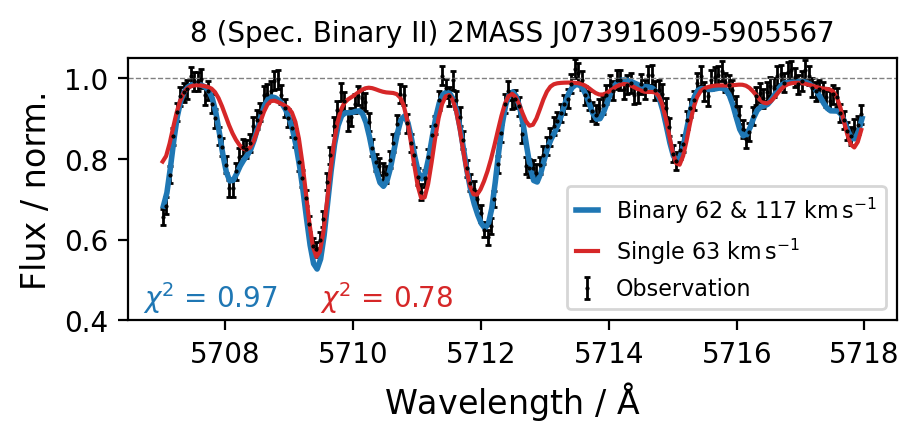
\includegraphics[width=\textwidth]{figures/examples_flag_sp_3.png}
 \caption{\textbf{Example spectrum for a double-lined spectroscopic binary star (SBII) that is better fit with our binary fitting algorithm.}} \label{fig:examples_flag_sp_3}
\end{figure}

\subsection{Fit optimization} \label{sec:caveats_fitting}

As described in Sec.~\ref{sec:allspec_analysis}, we are using the \textsc{curve\_fit} function of \texttt{scipy.optimize} \citep{scipy} to optimize the difference of observed and synthetic spectra, whose optimization can get stuck in local minima. We have tried to automatically identify regions of the parameter space where the \textsc{scipy.optimize.curve\_fit} function has gotten stuck. In particular for some red clump stars as well as cool giant stars with $T_\mathrm{eff} < 3750\,\mathrm{K}$ and $\log g < 0.5$ (see Sec.~\ref{sec:uncertainty_accuracy}), we have been able to recover a pattern of abundances being stuck around their initial value. However, this pattern is not consistent enough to flag stars without a significant amount of false-positives. Because of the zero point corrections, these are shifted away from the usual initial guess of $0\,\mathrm{dex}$ depending on the element (see zeropoints in Table~\ref{tab:zeropoints}).

Such a fitting failure would also be expected when applying \textit{The Payne} \citep{Ting2019} with its similar default setup that adopts parameter bounds for the fitting parameters and thus employs the \texttt{curve\_fit} function with the \textit{trust region reflective} (\texttt{trf}) method. Contrary to this, \textit{The Cannon} version by \citep{Casey2016} uses the \textsc{scipy.optimize.leastsq} fitting approach.

Given the common use of \texttt{curve\_fit}, future pipelines should test a range of approaches to avoid this issue. Firstly, instead of using \texttt{trf}, the \textit{Dogbox} (\texttt{dogbox}) method,  could be used. The method is potentially slower but more reliable for complex parameter spaces. It could be used to randomly check the convergence of the \texttt{trf} method or be applied only to regions where multiple local minima are expected.

Moving away from the \texttt{curve\_fit} function, the \textsc{differential\_evolution} function of the \texttt{scipy.optimize} module could be used for slow but global optimization. Finally, multiple randomized initial starting guesses could be applied for \texttt{curve\_fit}, but would multiply the computing costs linearly by the number of initial guesses.

Finally, the fitting optimization and uncertainty estimation should be performed in a more sophisticated Bayesian framework that folds in photometric, astrometric, and asteroseismic information and their uncertainties. We have indeed implemented such a framework with a likelihood estimate from spectroscopic information and prior information based on photometric, astrometric, and asteroseismic estimates for test purposes. When implementing the resulting posterior into the Markov-Chain Monte-Carlo machinery of \textsc{emcee} \citep{ForemanMackey2013}, we have not been able to limit the computational time (when fitting all labels) to a competitive level with \texttt{curve\_fit} and thus not implemented this approach for the analysis of a million spectra. We note, however, that a future analysis should implement this approach - either with \textsc{emcee} or another Bayesian inference engine like \textsc{UltraNest} \citep{Buchner2021}. Furthermore, we suggest to either separate the likelihood and posterior estimation steps \citep[see e.g.][]{Gent2022} or limit the optimization to only a few major stellar labels \citep[see e.g.][]{Traven2020}.

\subsection{Reliability of flags} \label{sec:caveats_flags}

We have tried to develop a quality assurance pipeline that automatically flags results and stars that may not be adequately analysed with our assumptions.

\subsubsection{Bug in \texttt{flag\_fe\_h}}

The quality flag for iron abundance, \texttt{flag\_fe\_h}, was computed similarly to the elemental abundances, that is, by comparing the best-fit spectrum with a spectrum with the lowest grid value. In the case of \feh, however, this is not the appropriate reference value. It had led to a comparison of a spectrum with $\mathrm{[Fe/H]} = -0.74\,\mathrm{dex}$ to one with the lowest grid value of $\mathrm{[Fe/H]} = -0.75\,\mathrm{dex}$, which can easily be too similar within the SNR range. This has affected up to 34\% of stars and we therefore do not recommend the use of this flag at all. In the future, such a test should be performed with respect to an actually low (undetectable) amount of iron, such as $\mathrm{[Fe/H]} = -4$.

\subsubsection{Fitting machinery stuck in local minimum}

As laid out in Sec.~\ref{sec:caveats_fitting}, we have not been able to automatically flag all estimates for which our fitting machinery has gotten stuck in local minima, most notably the initial value.

\subsubsection{Binary or fast rotating star?}

With the increasing number of turn-off stars as part of ongoing GALAH observations, we have tried to implement a more sensitive approach to identify binaries in this region. This may, however, mean that we have also introduced more false-positive detections of stars that are only fast rotating with higher \vsini, rather than being a binary system. We therefore suggest carefully considering using or neglecting the accompanying flag in GALAH DR4 (see Table~\ref{tab:flag_sp}).

\subsection{Summary of caveats} \label{sec:caveats_summary}

In summary, the most important caveats are:
\begin{itemize}
    \item Noding in \TLF around edges between neural networks: Our tests when switching between neural networks indicate that this effect for \TLF should stay within the precision uncertainties. A more difficult effect might be that some elements could be fit as part of one neural network based on the detectability tests that were performed at the grid centres of each neural network.
    \item Mismatches of photometry and spectroscopy: Both imperfect isochrone and spectrum models can drive a mismatch in the estimation of spectroscopic parameters. This is most notable around the secondary red clump region and also expected for highly extincted regions.
    \item Imperfect synthesis leading to trends in cool stars: The unreliable line data in cool stars is causing increasingly inaccurate models and inferred stellar properties towards the coolest stars.
    \item The coolest giant stars ($T_\mathrm{eff} < 3750\,\mathrm{K}$ and $\log g < 0.5$) still are rather unreliable.
    \item Lower precision for Eu due to missing masking of neural networks.
\end{itemize}

These caveats are the unfortunate negative effects of our successful attempt to increase the accuracy and precision of most stellar parameters and elemental abundances while simultaneously pushing the number of stars for which we can report abundances.

%%%%%%%%%%%%%%%%%%%%%%%%%%%%%%%%%%%%%%%%%%%%%%%%%%%%%%%%%%%%%%%%%%%%%%%%%
\section{CONCLUSIONS}
\label{sec:conclusion}

The GALAH survey celebrates its 10th anniversary with the release of GALAH DR4, marking a decade of significant contributions to our understanding of the Milky Way and the elemental composition of its stars. Over the years, GALAH has been instrumental in measuring and cataloging the chemical fingerprints of stars, which serve as cosmic barcodes that reveal their formation histories, migration patterns, and the evolutionary processes that shaped our Galaxy.

With GALAH DR4, we have improved upon the precision and accuracy of stellar parameters and elemental abundances for over a million stars. This release benefits from a decade of continuous development in spectroscopic techniques, calibration processes, and the adoption of cutting-edge models like 1D NLTE and even 3D NLTE synthesis for lithium abundances. The inclusion of photometric and astrometric information from \Gaia DR3 has further strengthened the reliability of stellar parameters, particularly for surface gravities, breaking long-standing degeneracies in spectroscopic data.

The unique value of GALAH lies in its detailed mapping of elements crucial to life as we know it. By tracking the abundances of carbon, nitrogen, and oxygen (CNO), as well as rare heavy elements used in modern electronics, GALAH has provided key insights into how the building blocks of life and technology were forged in the interiors of stars and distributed throughout the Milky Way over billions of years.

The next decade promises further improvements and discoveries as GALAH continues to push the boundaries of stellar spectroscopy. Upcoming surveys and future releases will likely address the caveats discussed in this work, refine the data products, and expand upon the wealth of knowledge already provided. The legacy of GALAH will undoubtedly continue to influence not only stellar and galactic archaeology but also our broader understanding of the cosmos and the elements that shape modern life.

%%%%%%%%%%%%%%%%%%%%%%%%%%%%%%%%%%%%%%%%%%%%%%%%%%%%%%%%%%%%%%%%%%%%%%%%%

%%%%%%%%%%%%%%%%%%%%%%%%%%%%%%%%%%%%%%%%%%%%%%%%%%
\section*{Acknowledgements}
%%%%%%%%%%%%%%%%%%%%%%%%%%%%%%%%%%%%%%%%%%%%%%%%%%

We acknowledge the traditional owners of the land on which the AAT and ANU stand, the Gamilaraay, the Ngunnawal and Ngambri people. We pay our respects to Elders, past and present, and are proud to continue their tradition of surveying the night sky in the Southern hemisphere.

We thank the staff at Siding Spring Observatory for their decade-long maintenance of 2dF-HERMES and support during observations, without whom this project would not have been possible: NAME1, NAME2, ...

This work was supported by the Australian Research Council Centre of Excellence for All Sky Astrophysics in 3 Dimensions (ASTRO 3D), through project number CE170100013. SB acknowledges support from the Australian Research Council under grant number DE240100150.

\section*{Facilities}

\textbf{AAT with 2dF-HERMES at Siding Spring Observatory:}
AAT observations for this data release were performed under programs {2013B/13}, {2014A/25}, {2015A/3}, {2015A/19}, {2015B/1}, {2015B/19}, {2016A/22}, {2016B/10}, {2016B/12}, {2017A/14}, {2017A/18}, {2017B/16}, {2018A/18}, {2018B/15}, {2019A/1}, {2019A/15}, {2020B/14}, {2020B/23}, {2022B/02}, {2022B/05}, {2023A/04}, {2023A/08}, {2023A/09}, {2023B/04}, and {2023B/05}.

\textbf{AAO Data Central:} This paper includes data that has been provided by AAO Data Central  (\url{datacentral.org.au}) and makes use of services and code that have been provided by AAO Data Central.

\textbf{\Gaia: } This work has made use of data from the European Space Agency (ESA) mission \Gaia (\url{http://www.cosmos.esa.int/gaia}), processed by the \Gaia Data Processing and Analysis Consortium (DPAC, \url{http://www.cosmos.esa.int/web/gaia/dpac/consortium}). Funding for the DPAC has been provided by national institutions, in particular the institutions participating in the \Gaia Multilateral Agreement. 

\textbf{Other facilities:} This publication makes use of data products from the Two Micron All Sky Survey \citep{Skrutskie2006} and the CDS VizieR catalogue access tool \citep{Vizier2000}.

\section*{Software}

The research for this publication was coded in \textsc{python} (version 3.7.4) and included its packages
\textsc{astropy} \citep[v. 3.2.2;][]{Robitaille2013,PriceWhelan2018},
\textsc{astroquery} \citep[v. 0.4;][]{Ginsburg2019},
\textsc{corner} \citep[v. 2.0.1;][]{corner},
\textsc{galpy} \citep[version 1.6.0;][]{Bovy2015},
\textsc{IPython} \citep[v. 7.8.0;][]{ipython},
\textsc{matplotlib} \citep[v. 3.1.3;][]{matplotlib},
\textsc{NumPy} \citep[v. 1.17.2;][]{numpy},
\textsc{scipy} \citep[version 1.3.1;][]{scipy},
\textsc{sklearn} \citep[v. 0.21.3;][]{scikit-learn},
We further made use of \textsc{topcat} \citep[version 4.7;][]{Taylor2005};


\bibliography{bib}

\appendix

\section{Initial parameters}

In this section, we append the overview of the initial and final stellar parameters of GALAH DR4. We show the density distribution of \logg, \feh, \vmic, and \vsini in each row as a function of \Teff. The columns show the same stars and their final parameters, the initial value, the reduction pipeline suggestion, the \Gaia DR3 \texttt{gspphot} estimates and the GALAH DR3 estimates, respectively.

\begin{figure*}[ht]
 \centering
 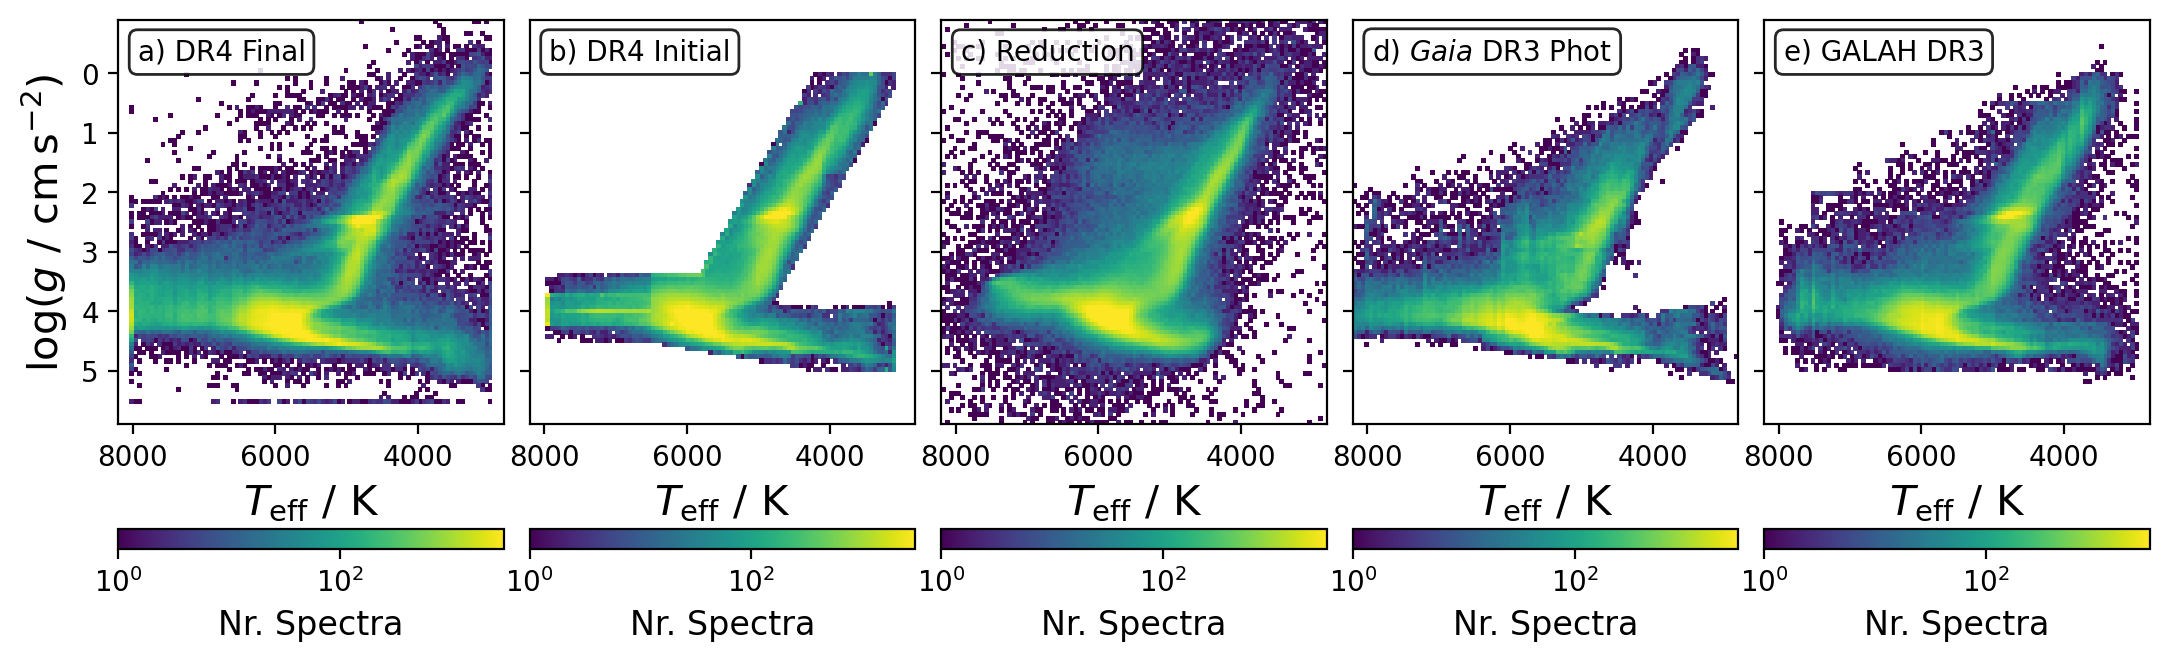
\includegraphics[width=\textwidth]{figures/initial_teff_logg.png}
 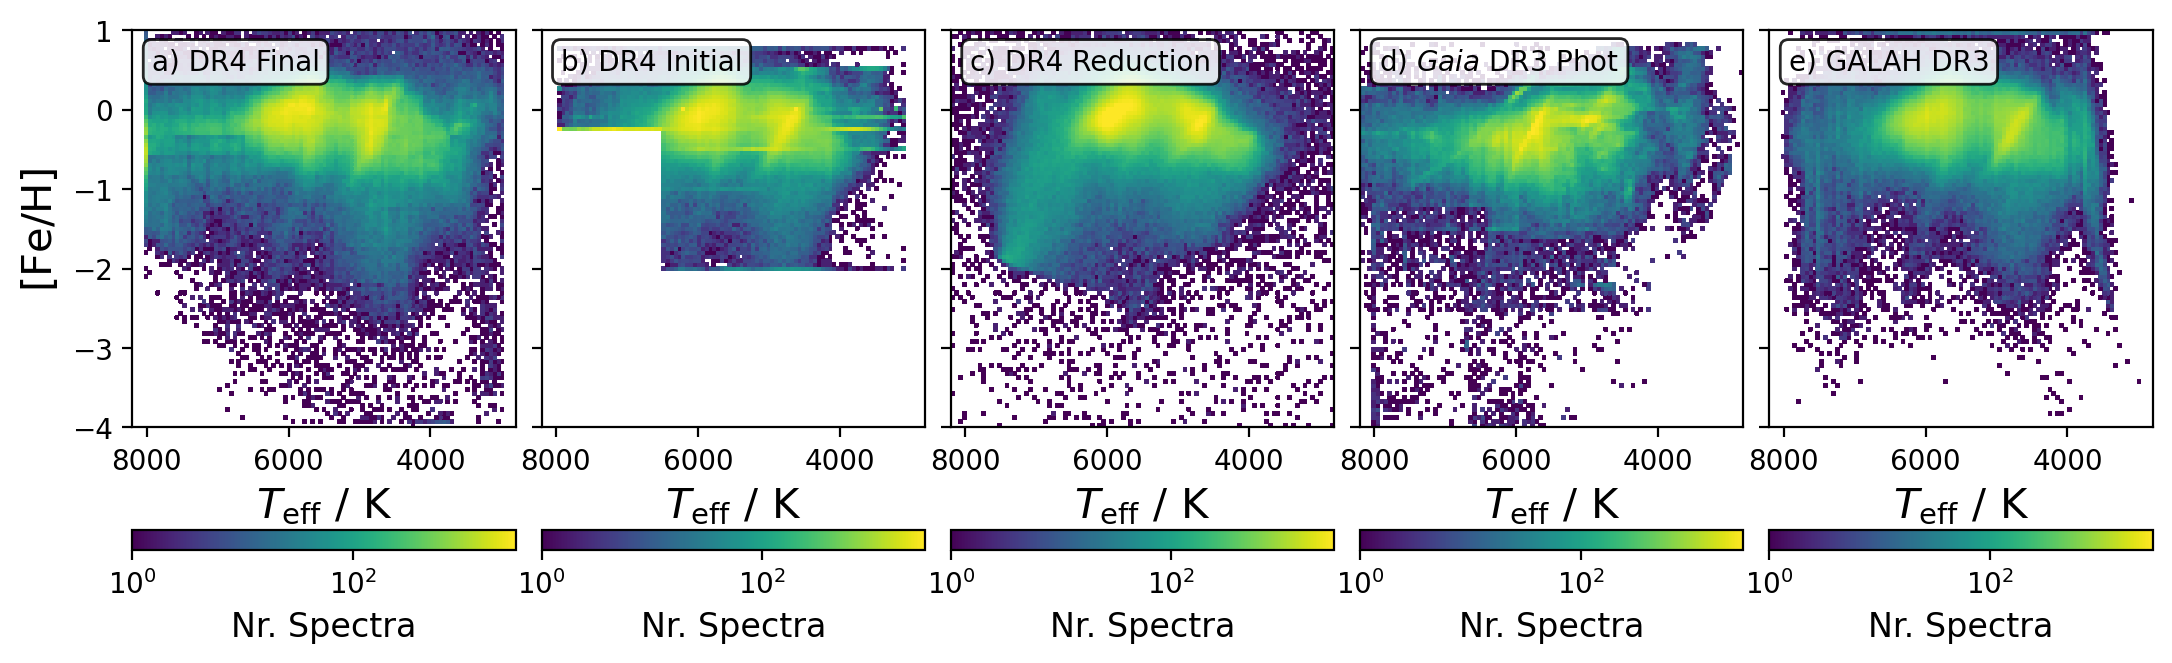
\includegraphics[width=\textwidth]{figures/initial_teff_fe_h.png}
 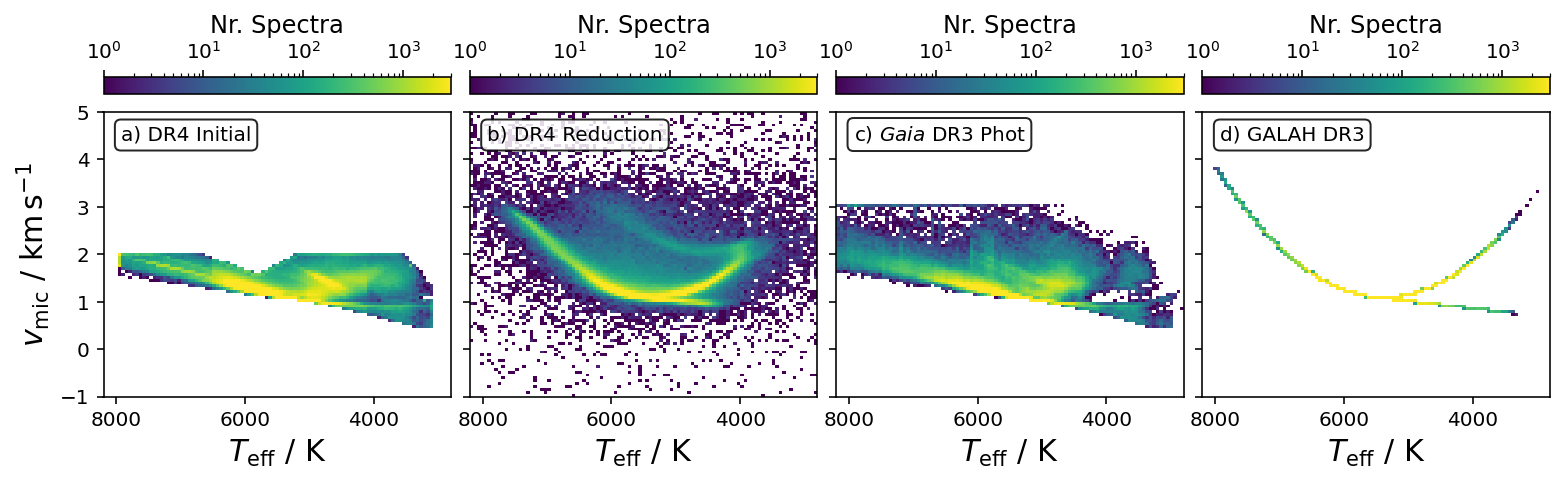
\includegraphics[width=\textwidth]{figures/initial_teff_vmic.png}
 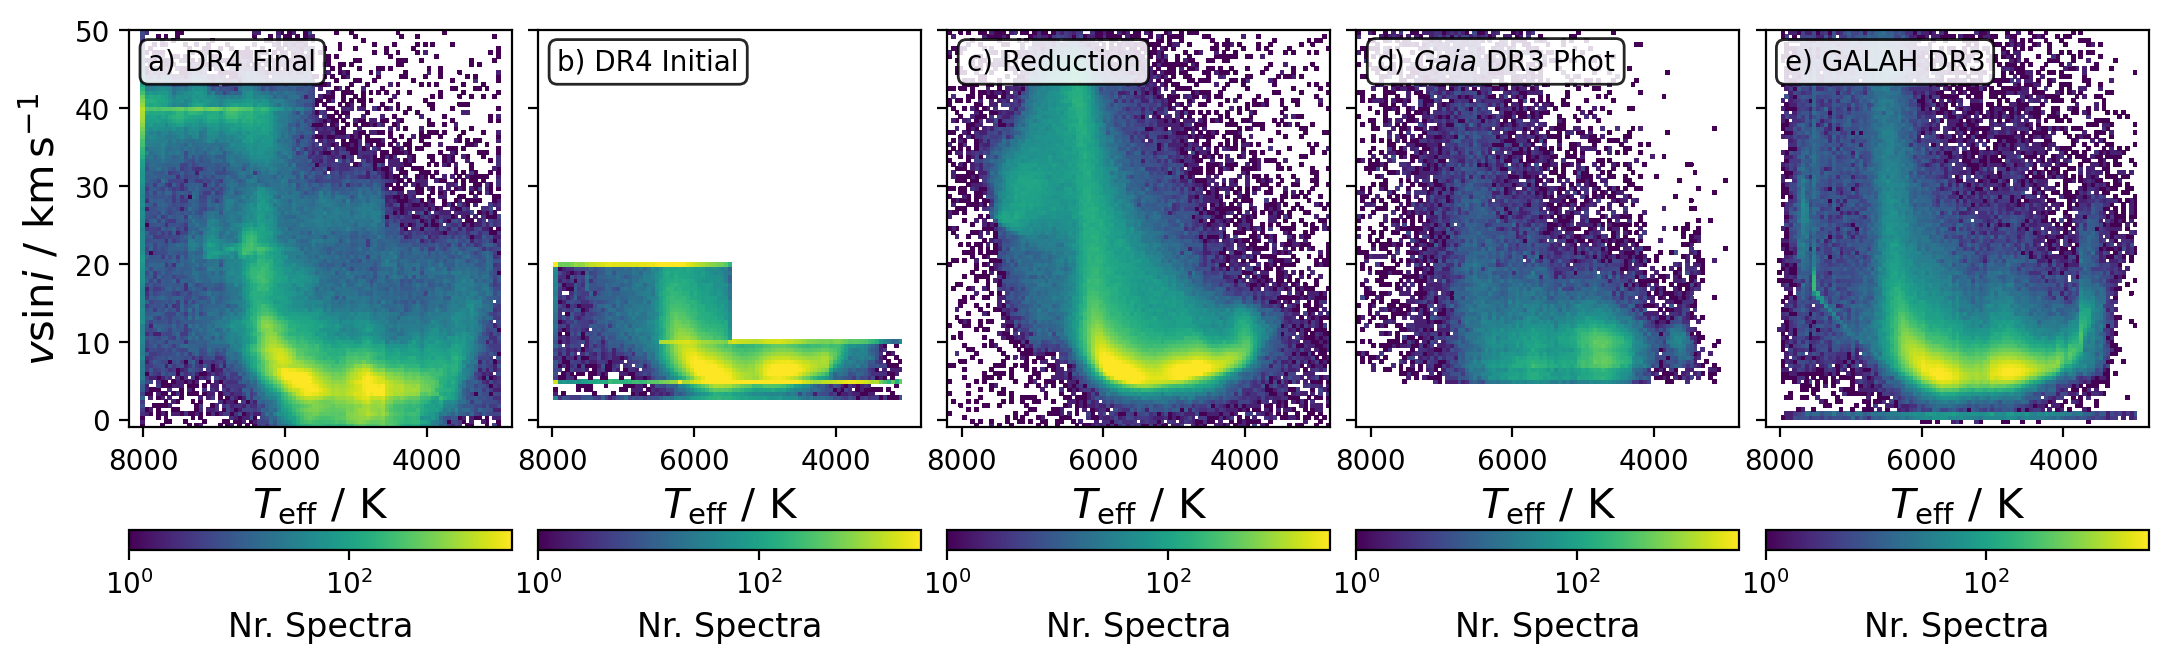
\includegraphics[width=\textwidth]{figures/initial_teff_vsini.png} \caption{\textbf{Comparison of final GALAH DR4 stellar parameters (first column) against the initial parameters used in the \textit{allstar} analysis (second column), estimates from the GALAH DR4 reduction pipeline (third column), \Gaia DR3 \citep[fourth column with \vmic based on the adjusted formula from ][]{DutraFerreira2016}, and GALAH DR3 (fifth column).}} \label{fig:initial_parameters}
\end{figure*}

\section{Data Products}

In this section, we append examples of data products of GALAH DR4 that were not already shown in the main manuscript. We present the shortened table schema of the \texttt{allstar} and \texttt{allspec} catalogues in Table~\ref{tab:main_catalog_schema}. In Fig.~\ref{fig:210115002201239_allstar_fit_comparison}, we show the automatically created fit comparison of the \texttt{allstar} module for Vesta (210115002201239). In Fig.~\ref{fig:covariance_vesta_arcturus}, we show examples of the covariance matrices for Vesta and Arcturus, as representative examples for main sequence and giant stars. We note that these covariance matrices are a direct output of \texttt{scipy.optimize.curve\_fit} and note scaled up to the final label uncertainties.

% Main catalogue table schema with reference:
% \label{tab:main_catalog_schema}
\begin{table*}[ht]
\centering
\caption{Table schema of the GALAH DR4 main catalogues. Columns that are part of \texttt{allspec}, but not \texttt{allstar} are listed below the middle line. For compactness, we have combined repetitive columns (for example with integers N). Detailed table schemas are available in the FITS headers of each catalogue file.}
\label{tab:main_catalog_schema}
\begin{tabular}{llll}
\hline \hline
Column & Description & Column & Description \\
\hline
sobject\_id & GALAH identifier & tmass\_id & 2MASS identifier \\ 
gaiadr3\_source\_id & Gaia DR3 source\_id & survey\_name & 2dF-HERMES Program \\ 
field\_id & GALAH Field ID & setup & allspec/allstar \\ 
mjd & Modified Julian Date & ra & propagated from Gaia DR3 \\ 
dec & propagated from Gaia DR3 & flag\_sp & Major spectroscopic quality bitmask flag \\ 
flag\_sp\_fit & Major fitting quality flag & opt\_loop & Nr of optimisation loops used for fitting \\ 
flag\_red & Quality bitmask flag of reduction pipeline & snr\_px\_ccdN & Average SNR for CCD N \\ 
chi2\_sp & Chi2 value of spectroscopic fitting & px\_used\_perc & Percentage of spectrum used for fit \\ 
model\_name & Used neural network for synthesis & closest\_model & Closest neural network for synthesis \\ 
comp\_time & Computation time spent on spectrum & fit\_global\_rv & RV fitted or fixed after co-adding? \\ 
rv\_comp\_1 & Radial velocity of primary source & e\_rv\_comp\_1 & Uncertainty of rv\_comp\_1 \\ 
rv\_comp\_2 & Radial velocity of potential secondary source & e\_rv\_comp\_2 & Uncertainty of rv\_comp\_1 \\ 
rv\_gaia\_dr3 & Radial velocity in Gaia DR3 & e\_rv\_gaia\_dr3 & Uncertainty of rv\_gaia\_dr3 \\ 
v\_bary\_eff & Barycentric velocity correction & teff & Spectr. effective temperature \\ 
e\_teff & Uncertainty teff & logg & Photometric surface gravity \\ 
e\_logg & Uncertainty logg\_plx & fe\_h & Abundance of Fe as pseudo-metallicity \\ 
e\_fe\_h & Uncertainty fe\_h & flag\_fe\_h & Quality flag fe\_h \\ 
vmic & Microturbulence velocity (fitted) & e\_vmic & Uncertainty vmic \\ 
vsini & Broadening velocity & e\_vsini & Uncertainty of vsini \\ 
nn\_li\_fe & Elemental abundance for [Li/Fe] & nn\_e\_li\_fe & Uncertainty Li\_fe \\ 
nn\_flag\_li\_fe & Quality bitmask flag of Li\_fe & x\_fe & Elemental abundance for [X/Fe] \\ 
e\_x\_fe & Uncertainty of elemental abundance [X/Fe] & flag\_x\_fe & Quality bitmask flag of [X/Fe] \\ 
mass & Mass used for calculating logg(plx) & age & Age estimated when calculating mass \\ 
bc\_ks & Bolometric Correction of Ks band & a\_ks & Attenuation in Ks-band A(Ks) \\ 
lbol & Bolometric Luminosity & r\_med & Median Distance \\ 
r\_lo & Lower Limit Distance & r\_hi & Higher Limit Distance \\ 
sb2\_rv\_N & Nth perc. of RV residual signal & ew\_h\_beta & Equivalent Width of observed Hbeta core \\ 
ew\_h\_alpha & Equivalent Width of observed Halpha core & res\_h\_beta & Residual EW in Hbeta core \\ 
res\_h\_alpha & Residual EW in Halpha core & ew\_k\_is & EW of K7699 Interstellar Line \\ 
sigma\_k\_is & Gaussian sigma of K7699 Interstellar Line & rv\_k\_is & RV of K7699 Interstellar Line \\ 
ew\_dib5780 & Equivalent width of DIB NNNN & sigma\_dib5780 & Gaussian sigma of DIB NNNN \\ 
rv\_dib5780 & RV of DIB NNNN & ebv & Extinction E(B-V) \\ 
phot\_g\_mean\_mag & Mean Gaia DR3 G-band apparent magnitude & bp\_rp & Color of BP-RP bands \\ 
j\_m & 2MASS J-band magnitude & j\_msigcom & Uncertainty of j\_m \\ 
h\_m & 2MASS H-band magnitude & h\_msigcom & Uncertainty of h\_m \\ 
ks\_m & 2MASS Ks-band magnitude & ks\_msigcom & Uncertainty of ks\_m \\ 
W2mag & AllWISE W2-band magnitude & e\_W2mag & uncertainty of W2mag \\ 
ruwe & RUWE reported by Gaia DR3 & parallax & Astrometric parallax used for GALAH DR4 \\ 
parallax\_error & Uncertainty of astrometric parallax & ew\_li & Eqiuvalent width of Lithium 6708 LiI line \\ 
e\_ew\_li\_low & Lower uncertainty ew\_li & e\_ew\_li\_upp & Upper uncertainty ew\_li \\ 
a\_li & Absolute 3D NLTE Li abundance & a\_li\_upp\_lim & Upper limit of absolute 3D NLTE A(Li) \\ 
e\_a\_li\_low & Lower uncertainty of a\_li & e\_a\_li\_upp & Upper uncertainty of a\_li \\ 
e\_a\_li\_teff & Uncertainty of A(Li) due to temperature & flag\_a\_li & Flag for a\_li measurement \\ 
\hline
rv\_comp\_nr & Nr RV cross-correlation function peaks & rv\_comp\_1\_p & Prominence of rv\_comp\_1 in CCF \\ 
rv\_comp\_2\_h & Height of rv\_comp\_1 in CCF & rv\_comp\_2\_p & Prominence of rv\_comp\_1 in CCF \\ 
logg\_spec & Spectroscopic surface gravity estimate & e\_logg\_spec & Uncertainty logg\_spec \\ 
\hline
\end{tabular}
\end{table*}

\begin{figure*}[ht]
 \centering
 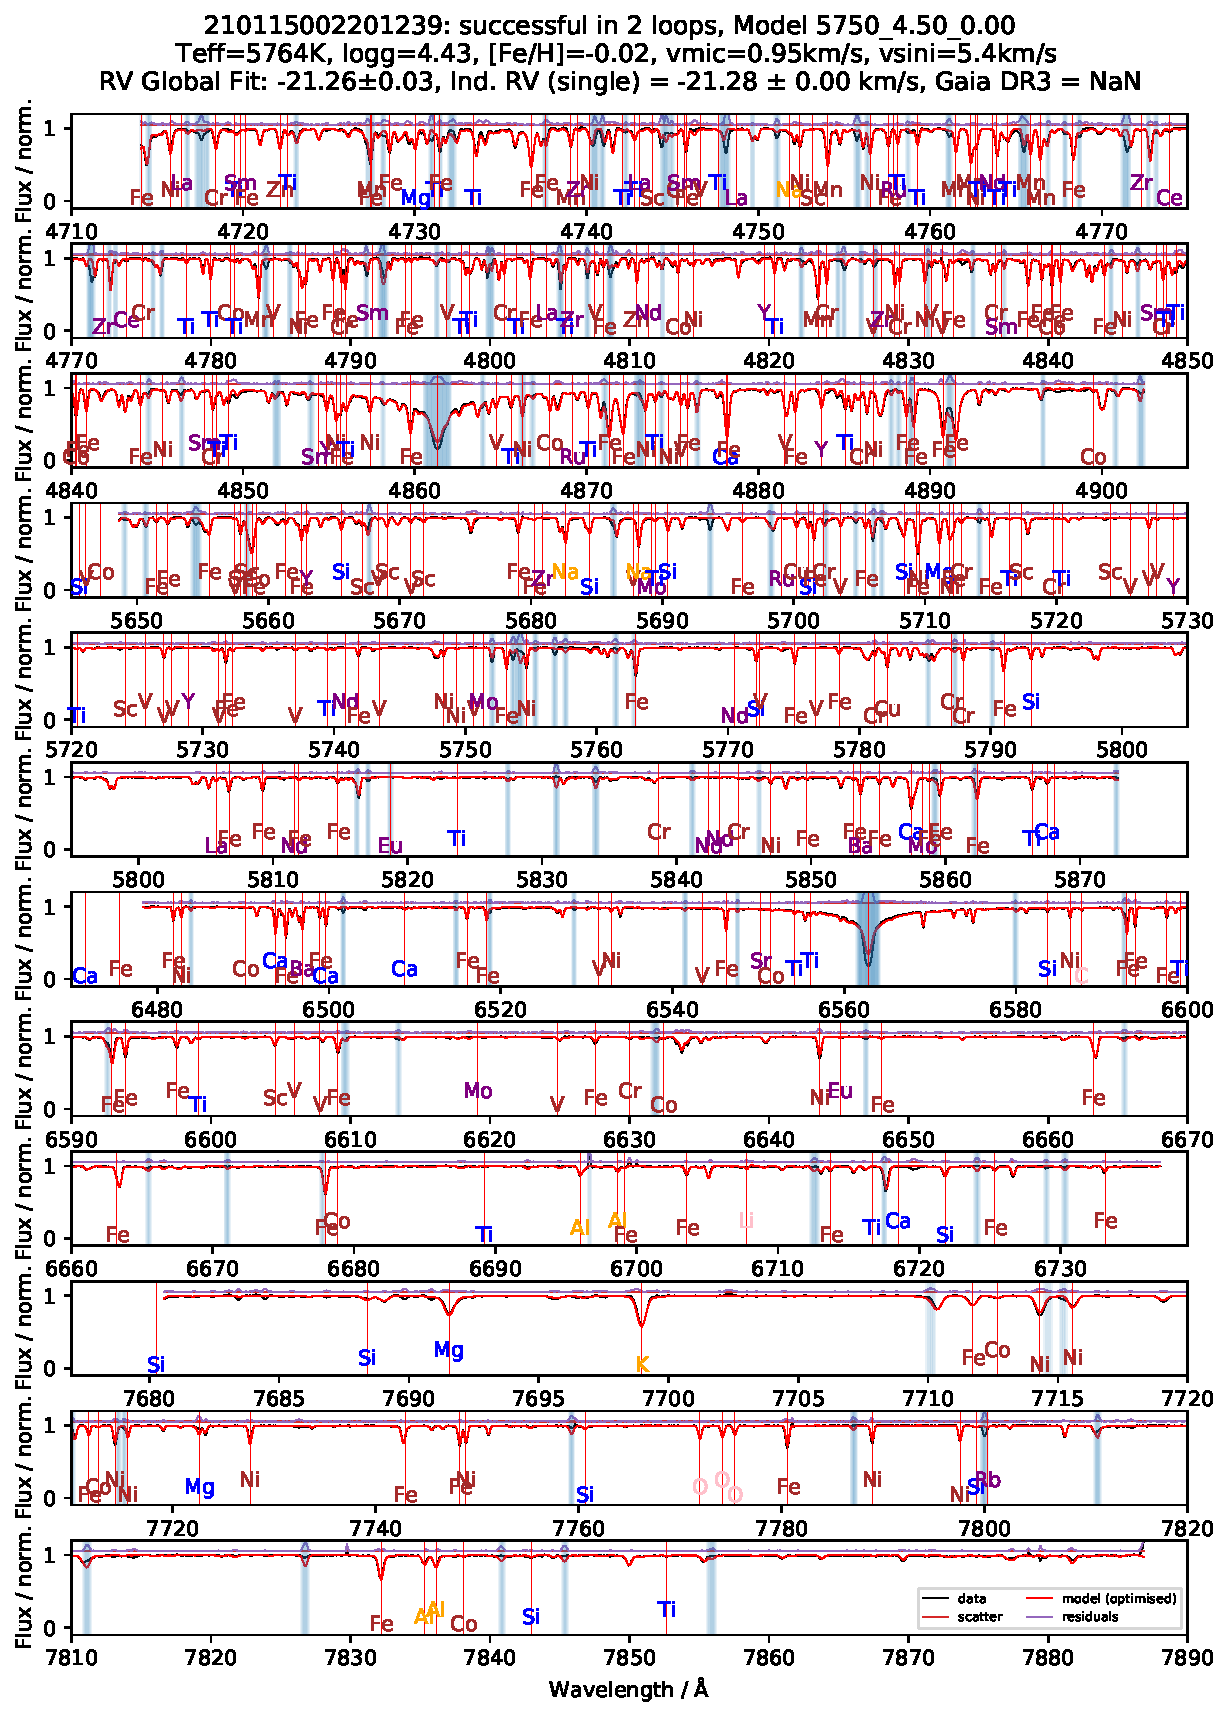
\includegraphics[width=0.9\textwidth]{figures/210115002201239_allstar_fit_comparison.pdf} \caption{\textbf{Example output of the \texttt{allstar} fitting routine for Vesta / 210115002201239.}} \label{fig:210115002201239_allstar_fit_comparison}
\end{figure*}

\begin{figure}[ht]
 \centering
 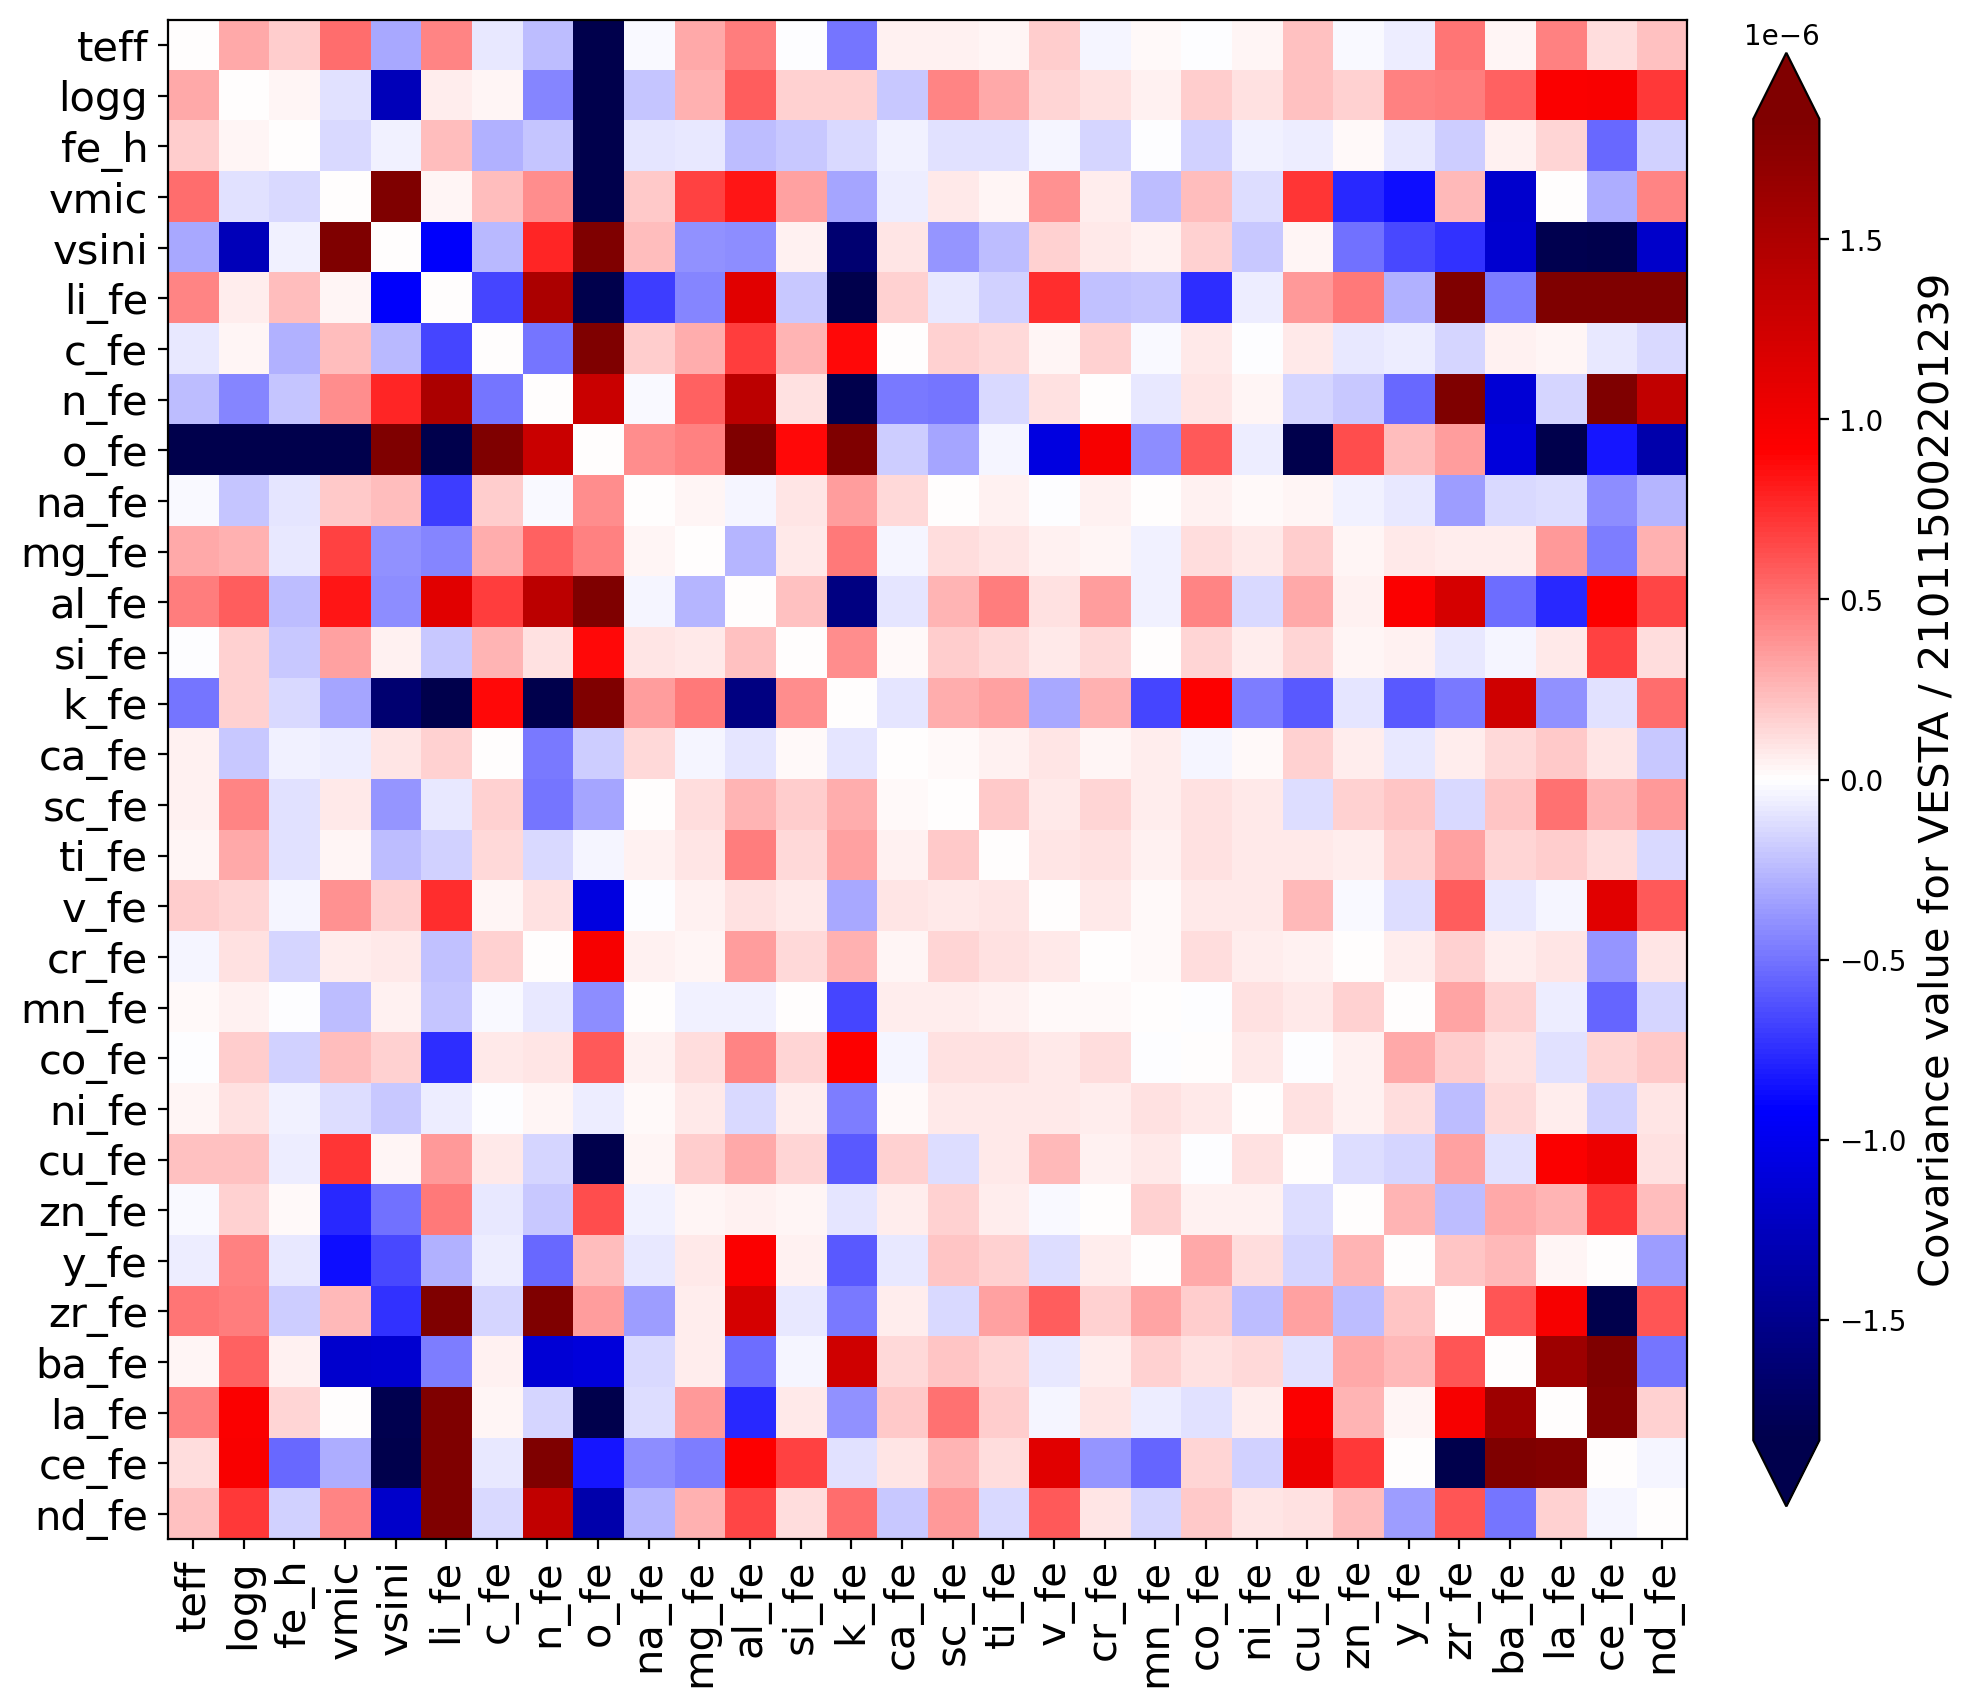
\includegraphics[width=\textwidth]{figures/covariance_vesta.png}
 \hfill
 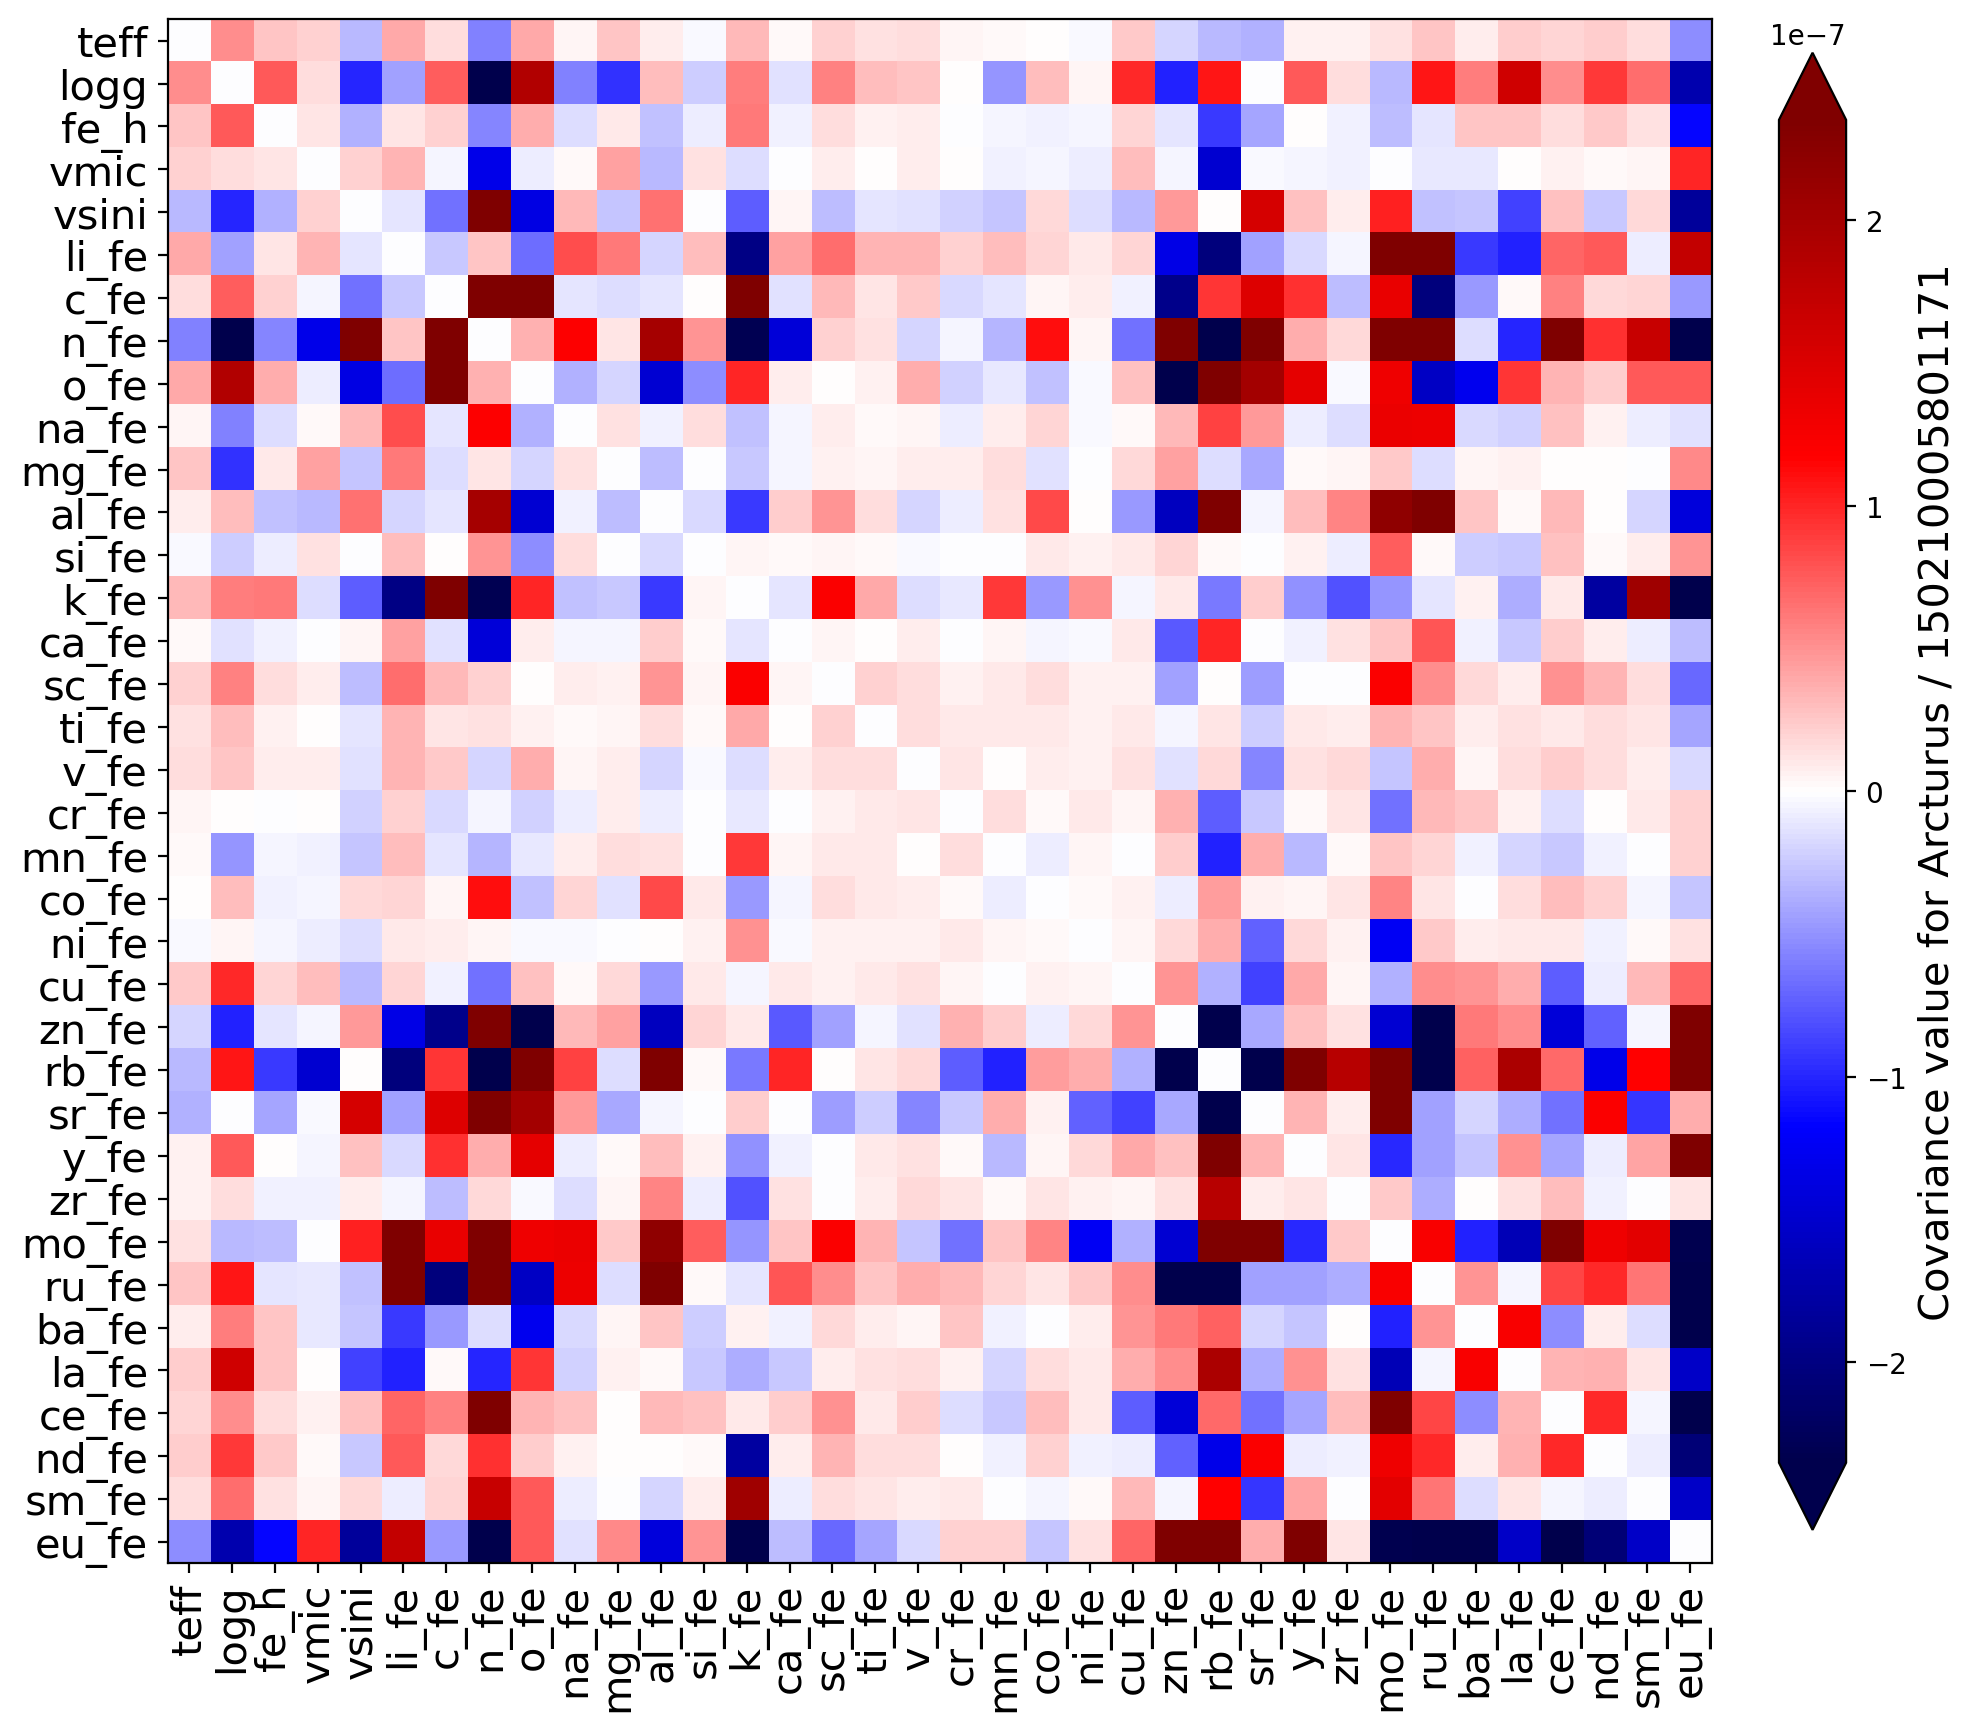
\includegraphics[width=\textwidth]{figures/covariance_arcturus.png}
 \caption{\textbf{Covariance matrices for labels for Vesta (panel a) and Arcturus (panel b).}}
 \label{fig:covariance_vesta_arcturus}
\end{figure}

\section{Stellar parameter and abundance validation}

\subsection{Accuracy}

We list the final stellar parameter and abundance zeropoints of the \texttt{allstar} modlue in Table~\ref{tab:zeropoints}. A complete table, including the zeropoints for the \texttt{allspec} module can be found as FITS file in the online \href{https://github.com/svenbuder/GALAH_DR4/blob/main/catalogs/galah_dr4_zeropoints_240705.fits}{repository}. As discussed in Sec.~\ref{sec:uncertainty_accuracy}, the choice of abundance zeropoints was made as a compromise between the different accuracy indicators shown in Fig.~\ref{fig:galah_dr4_zeropoint_checks_allstar} for the \texttt{allstar} module.

% Zeropoints table with \label{tab:zeropoints}
\begin{table}[ht]
\centering
\caption{Zero point estimates and corrections applied to the \texttt{allstar} measurements. We used \citet{Prsa2016} as reference for Solar parameters and \citet{Grevesse2007}, consistent with the \marcs model atmosphere composition \citep{Gustafsson2008}, as reference for Solar abundances. For reference, we also show the combined rotational and macroturbulence as well as microturbulence velocities from \citet{Jofre2014}. Values for Vesta indicate our uncorrected measurements for the Vesta spectrum.}
\label{tab:zeropoints}
\begin{tabular}{cccccc}
\hline \hline
Property & Reference & Zeropoint & Shift & Vesta & $\Delta$Vesta \\
& $R$ & $Z$ & $Z-R$ & $V$ & $V - R$ \\
\hline
\Teff & 5772.0 & 5772.0 & 0.0 & 5752.261 & -19.739 \\
\logg & 4.438 & 4.438 & 0.0 & 4.429 & -0.009 \\
\feh & 0.0 & 0.049 & 0.049 & -0.019 & -0.068 \\
A(Fe) & 7.45 & 7.499 & 0.049 & 7.431 & -0.068 \\
\vmic & 1.06 & 1.06 & 0.0 & 1.0 & -0.06 \\
\vsini & 4.5 & 4.5 & 0.0 & 5.552 & 1.052 \\
A(Li) & 1.05 & 1.05 & 0.0 & 1.108 & 0.058 \\
A(C) & 8.39 & 8.393 & 0.003 & 8.348 & -0.045 \\
A(N) & 7.78 & 7.705 & -0.075 & 8.368 & 0.663 \\
A(O) & 8.66 & 8.659 & -0.001 & 8.784 & 0.125 \\
A(Na) & 6.17 & 5.999 & -0.171 & 6.35 & 0.351 \\
A(Mg) & 7.53 & 7.445 & -0.085 & 7.687 & 0.242 \\
A(Al) & 6.37 & 6.185 & -0.185 & 6.552 & 0.367 \\
A(Si) & 7.51 & 7.486 & -0.024 & 7.515 & 0.029 \\
A(K) & 5.08 & 5.029 & -0.051 & 5.108 & 0.079 \\
A(Ca) & 6.31 & 6.287 & -0.023 & 6.361 & 0.074 \\
A(Sc) & 3.17 & 3.167 & -0.003 & 3.12 & -0.047 \\
A(Ti) & 4.9 & 4.876 & -0.024 & 4.882 & 0.006 \\
A(V) & 4.0 & 4.124 & 0.124 & 3.849 & -0.275 \\
A(Cr) & 5.64 & 5.64 & 0.0 & 5.61 & -0.03 \\
A(Mn) & 5.39 & 5.289 & -0.101 & 5.494 & 0.205 \\
A(Co) & 4.92 & 5.05 & 0.13 & 4.771 & -0.279 \\
A(Ni) & 6.23 & 6.228 & -0.002 & 6.236 & 0.008 \\
A(Cu) & 4.21 & 4.418 & 0.208 & 4.002 & -0.416 \\
A(Zn) & 4.6 & 4.651 & 0.051 & 4.53 & -0.121 \\
A(Rb) & 2.6 & 2.6 & 0.0 & -- & -- \\
A(Sr) & 2.92 & 2.92 & 0.0 & -- & -- \\
A(Y) & 2.21 & 2.204 & -0.006 & 2.152 & -0.052 \\
A(Zr) & 2.58 & 2.58 & 0.0 & 2.122 & -0.458 \\
A(Mo) & 1.92 & 1.92 & 0.0 & -- & -- \\
A(Ru) & 1.84 & 1.84 & 0.0 & -- & -- \\
A(Ba) & 2.17 & 2.108 & -0.062 & 2.113 & 0.005 \\
A(La) & 1.13 & 1.19 & 0.06 & 0.986 & -0.204 \\
A(Ce) & 1.7 & 1.77 & 0.07 & 1.447 & -0.323 \\
A(Nd) & 1.45 & 1.328 & -0.122 & 1.276 & -0.052 \\
A(Sm) & 1.0 & 1.0 & 0.0 & -- & -- \\
A(Eu) & 0.52 & 0.52 & 0.0 & -- & -- \\
\hline
\end{tabular}
\end{table}

\begin{figure*}[ht]
 \centering
 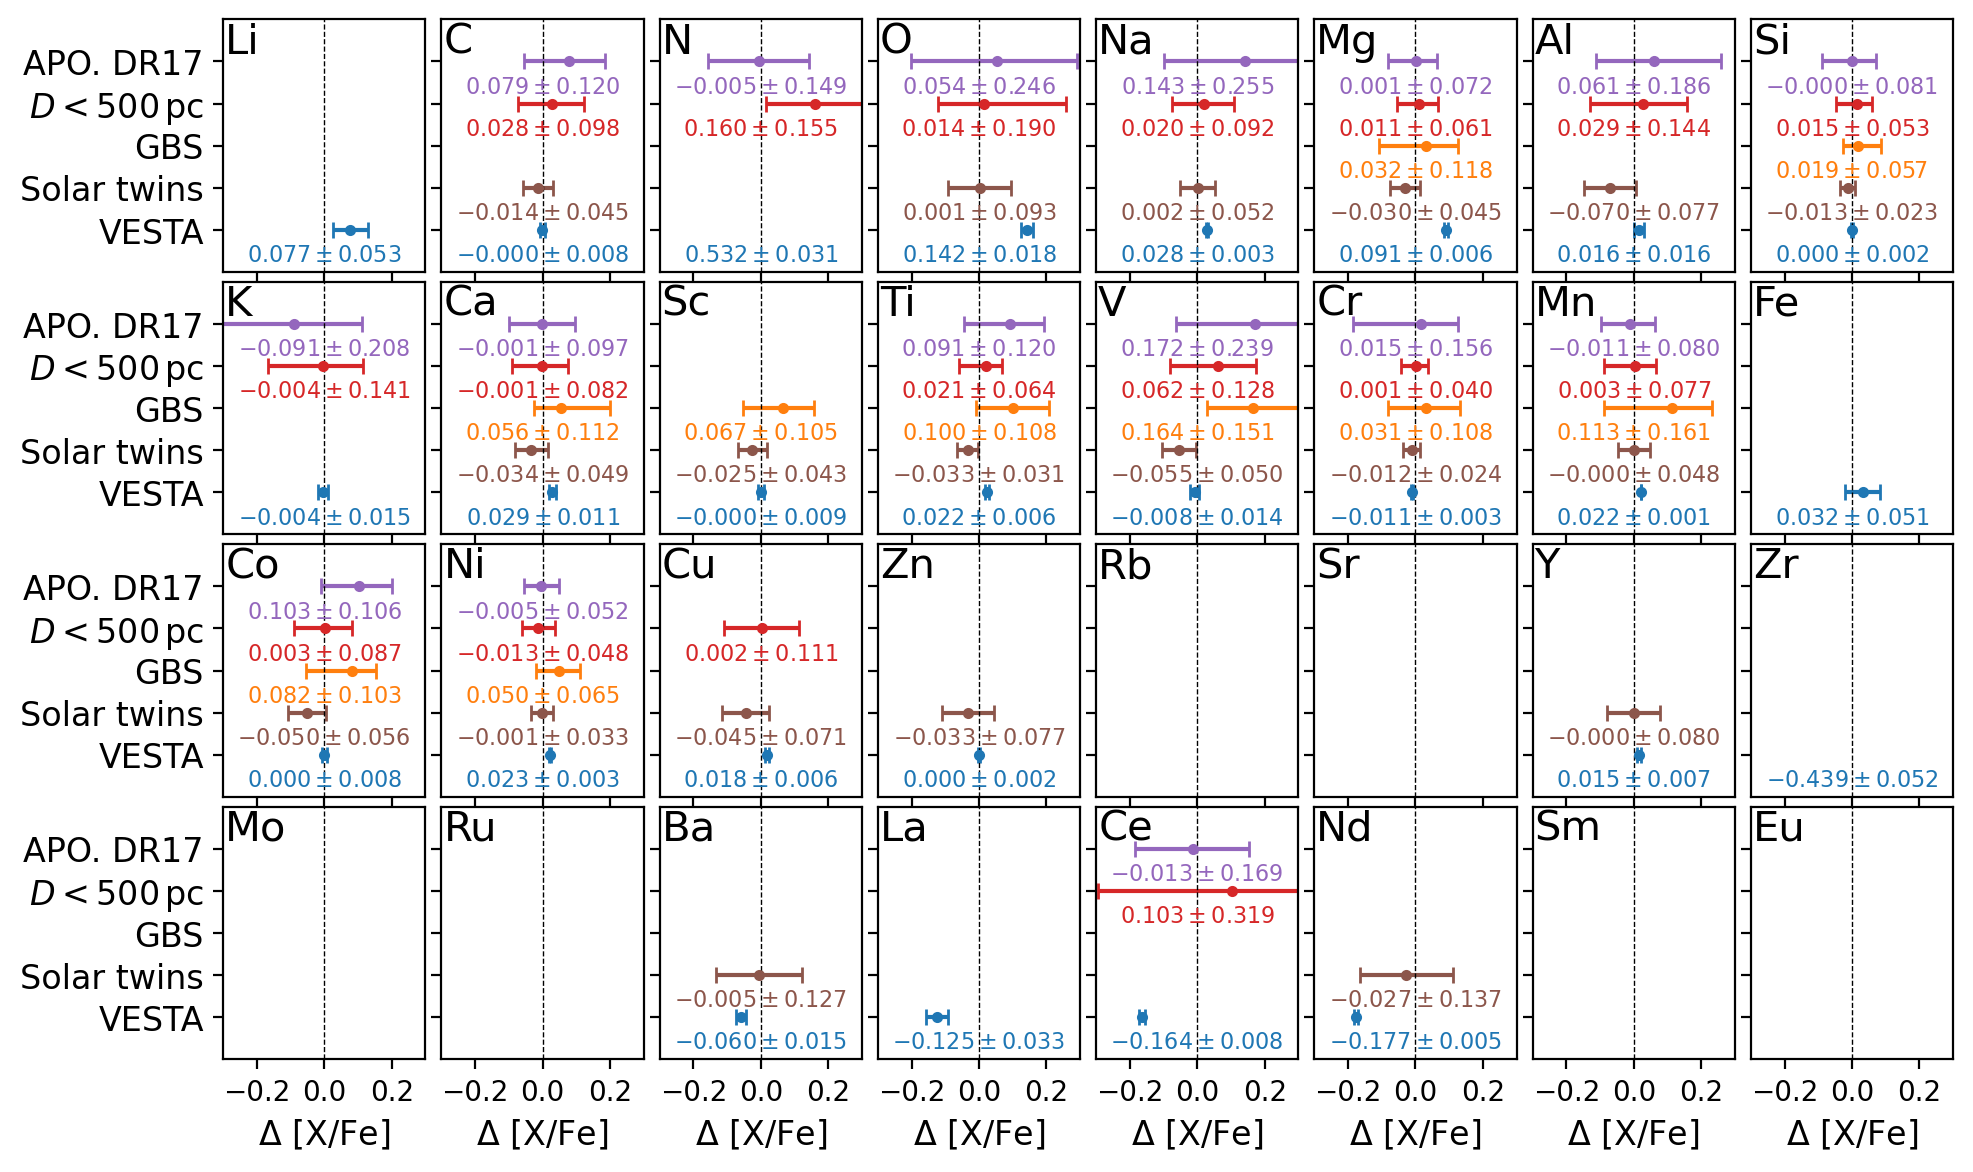
\includegraphics[width=\textwidth]{figures/galah_dr4_zeropoint_checks_allstar.png}
 \caption{\textbf{Zeropoint estimates of elemental abundances for GALAH DR4.}. Each panel shows the comparison to literature (DR4 - literature) for Vesta (blue), \Gaia FKG Benchmark Stars (orange), Stars with $\vert \mathrm{[Fe/H]} \vert \leq 0.1$ closer than $D_\varpi < 0.5\,\mathrm{kpc}$ (red), as well as stars that were also observed by APOGEE DR17 (purple).}
 \label{fig:galah_dr4_zeropoint_checks_allstar}
\end{figure*}

\subsection{Precision}

Fig.~\ref{fig:galah_dr4_precision_abundances}

\begin{figure*}[ht]
 \centering
 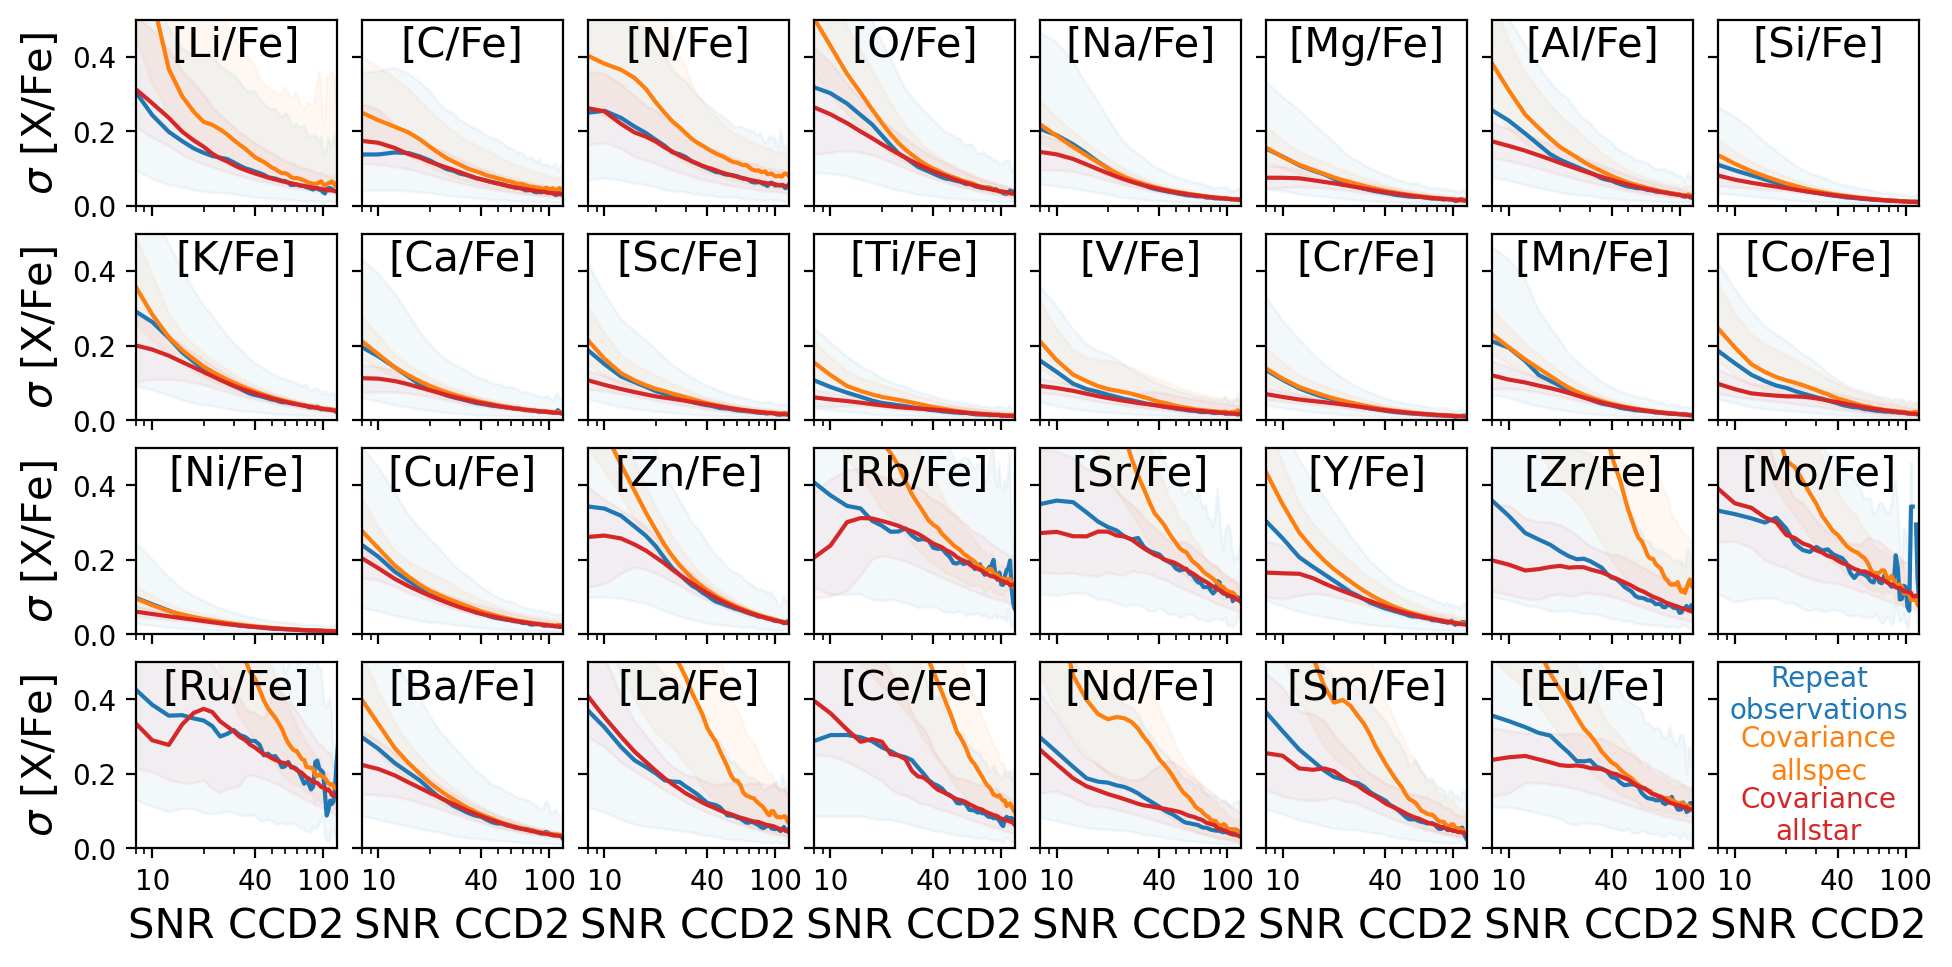
\includegraphics[width=\textwidth]{figures/galah_dr4_precision_abundances.png}
 \caption{\textbf{Precision monitoring of elemental abundances as a function of SNR for the green CCD2 across for GALAH DR4.}. Each panel shows the behavior for bins of width 10 for the scatter of repeat observations of the \texttt{allspec} runs (blue) as well as covariance uncertainties of \texttt{allspec} (orange) and \texttt{allstar} (red) setups.}
 \label{fig:galah_dr4_precision_abundances}
\end{figure*}

\begin{figure*}[ht]
 \centering
 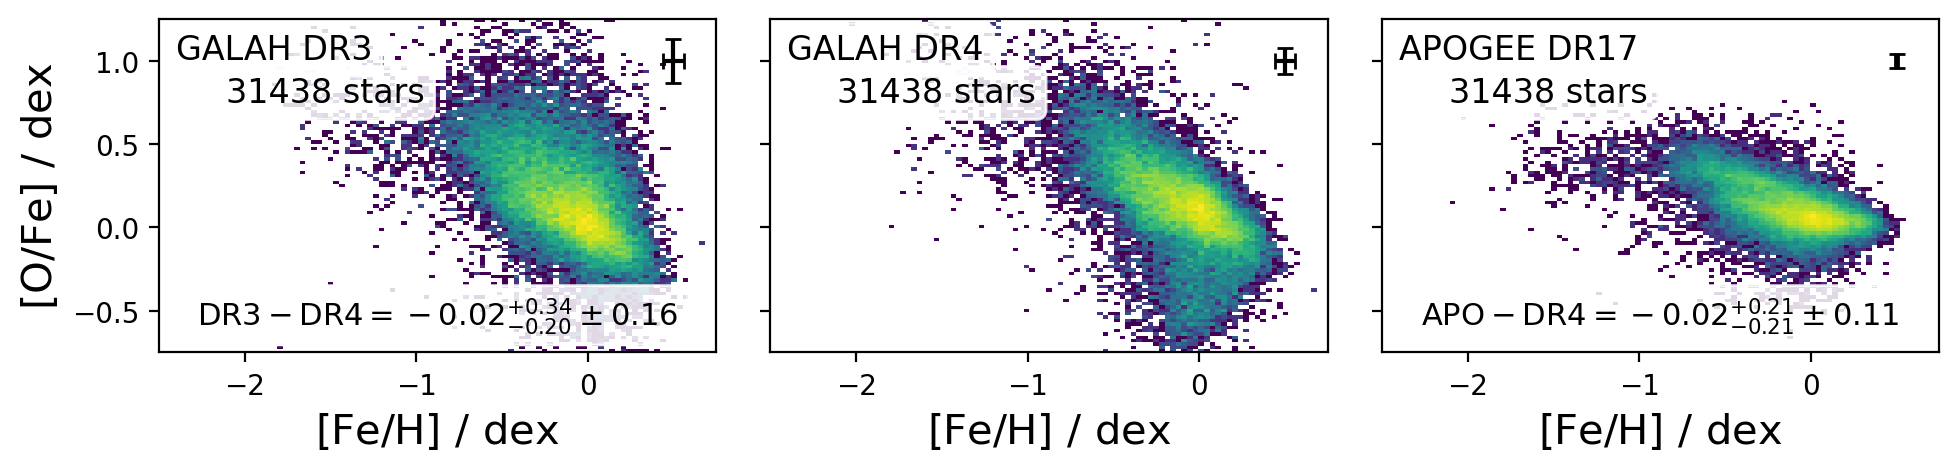
\includegraphics[width=0.87\textwidth]{figures/comparison_dr4_dr3_apo17_O_fe.png}
 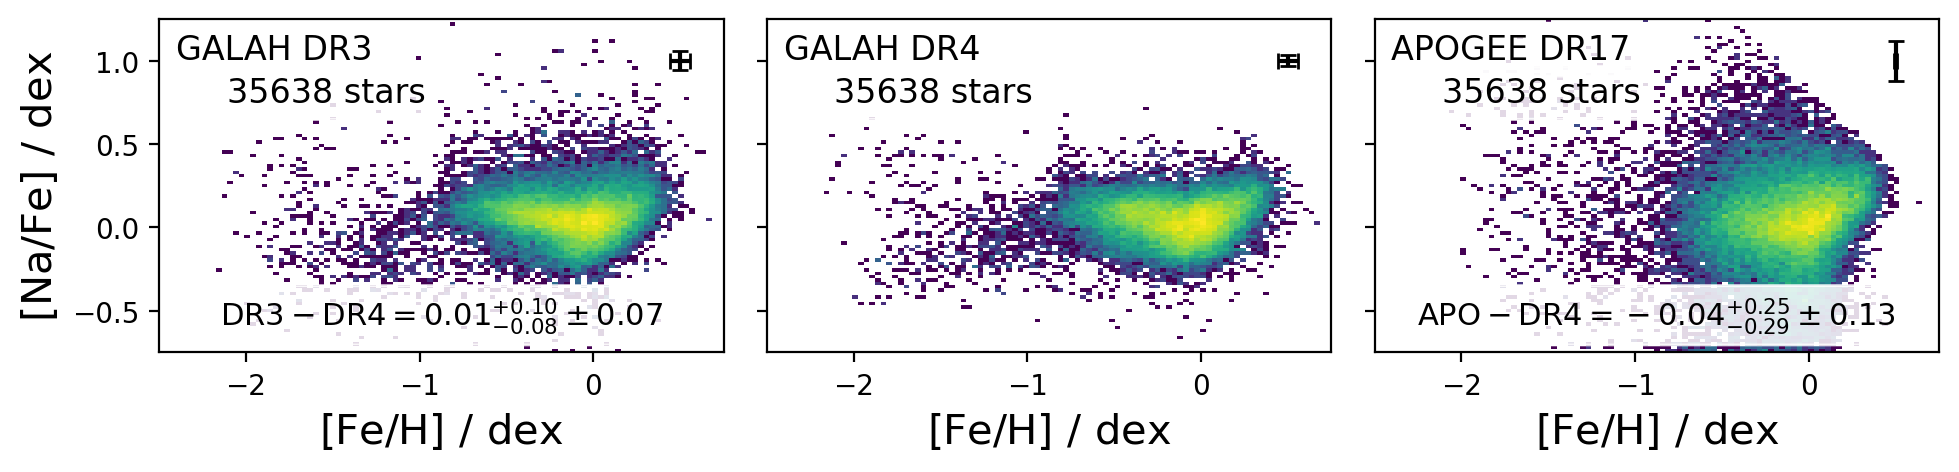
\includegraphics[width=0.87\textwidth]{figures/comparison_dr4_dr3_apo17_Na_fe.png}
 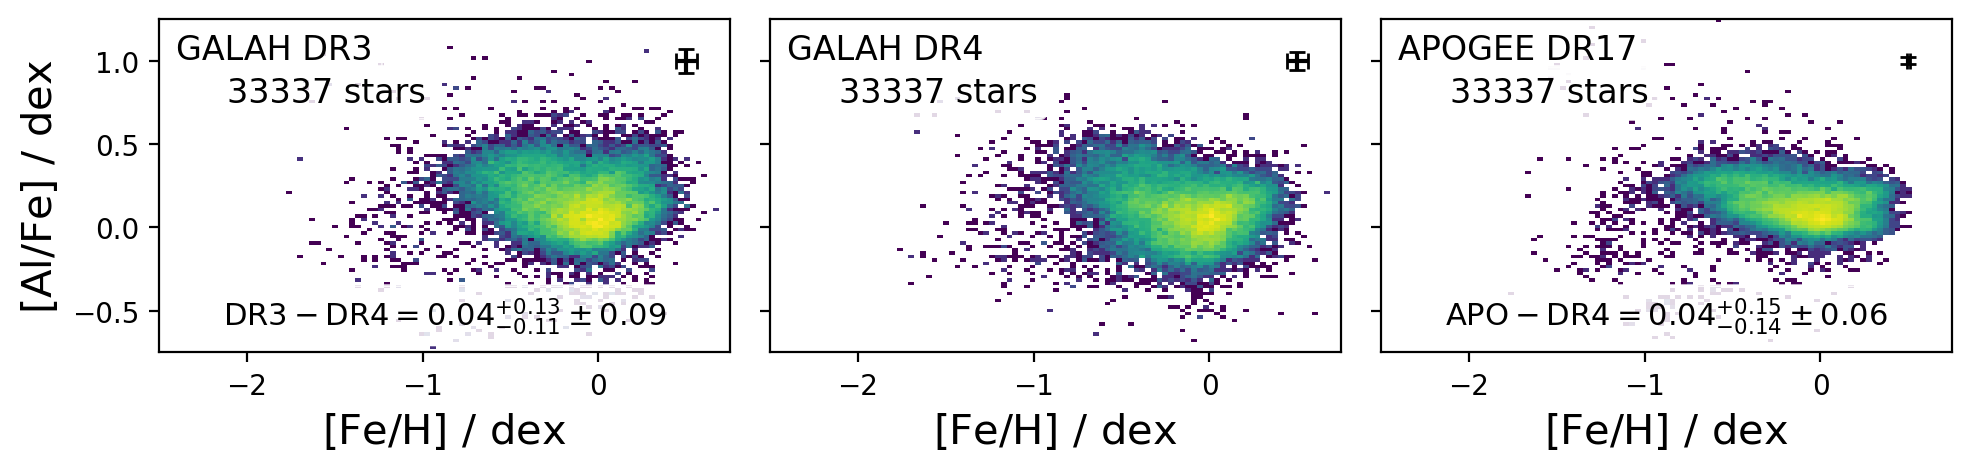
\includegraphics[width=0.87\textwidth]{figures/comparison_dr4_dr3_apo17_Al_fe.png}
 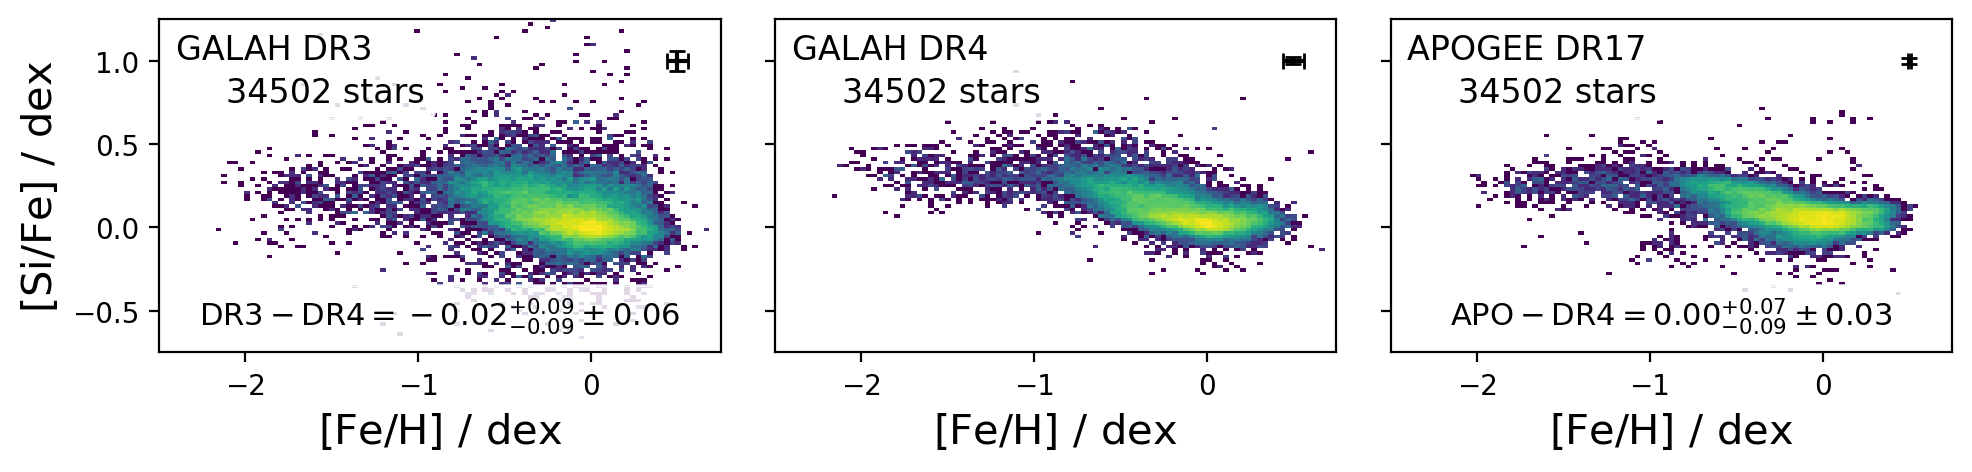
\includegraphics[width=0.87\textwidth]{figures/comparison_dr4_dr3_apo17_Si_fe.png}
 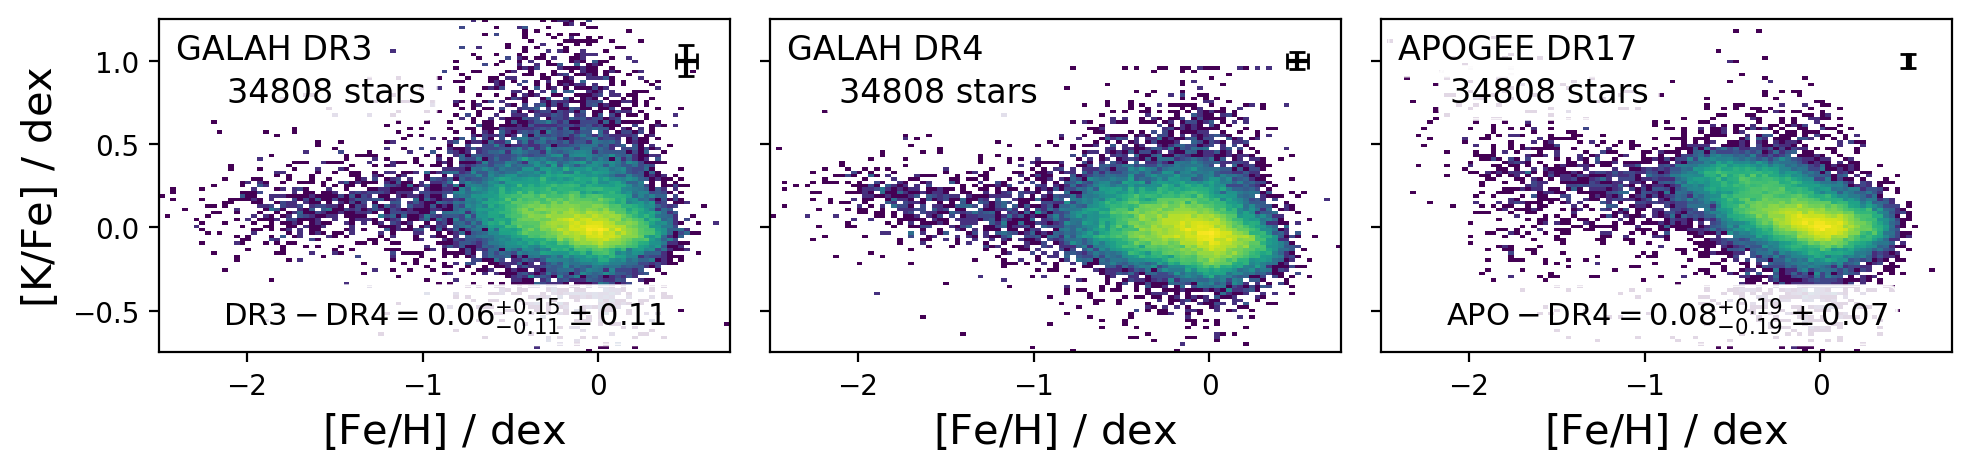
\includegraphics[width=0.87\textwidth]{figures/comparison_dr4_dr3_apo17_K_fe.png}
 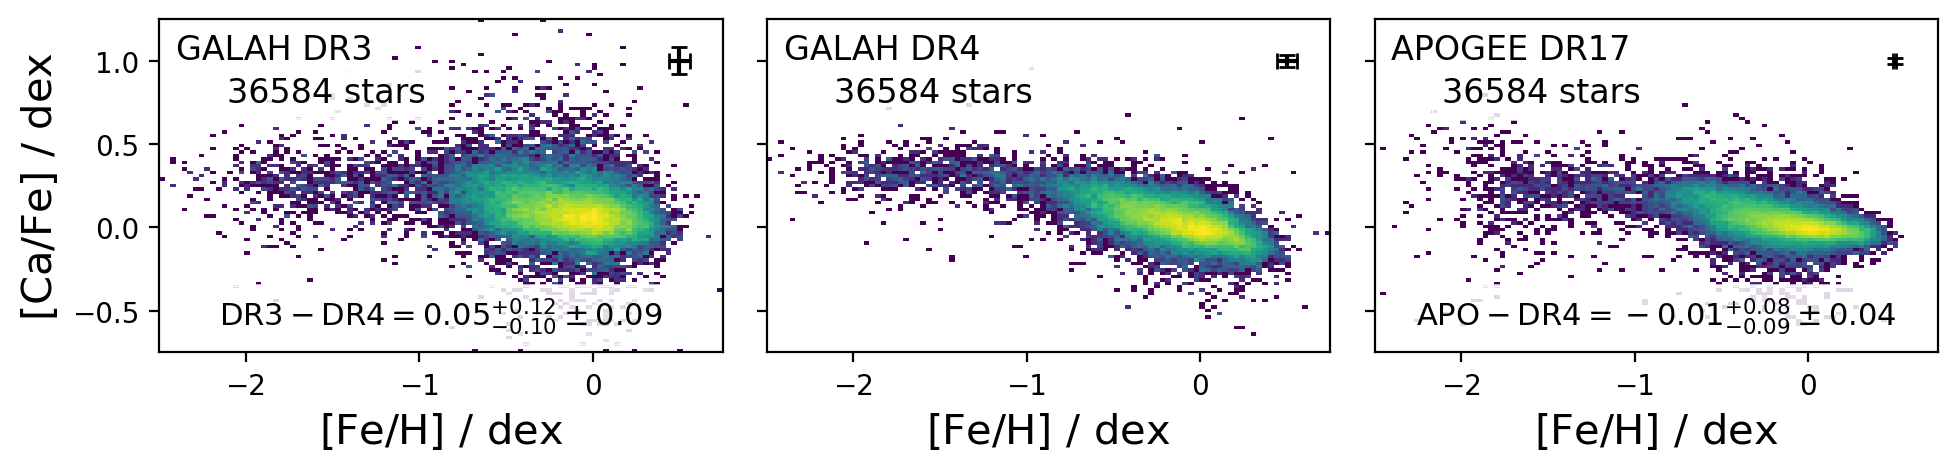
\includegraphics[width=0.87\textwidth]{figures/comparison_dr4_dr3_apo17_Ca_fe.png}
 \caption{\textbf{Comparison of stars with available measurements in GALAH DR3 (left column), GALAH DR4 (middle column) and APOGEE DR17 (right) for O, Na, Al, Si, K, and Ca}.}
 \label{fig:comparison_dr3_dr4_apo17_rest}
\end{figure*}


\begin{figure*}[ht]
 \centering
 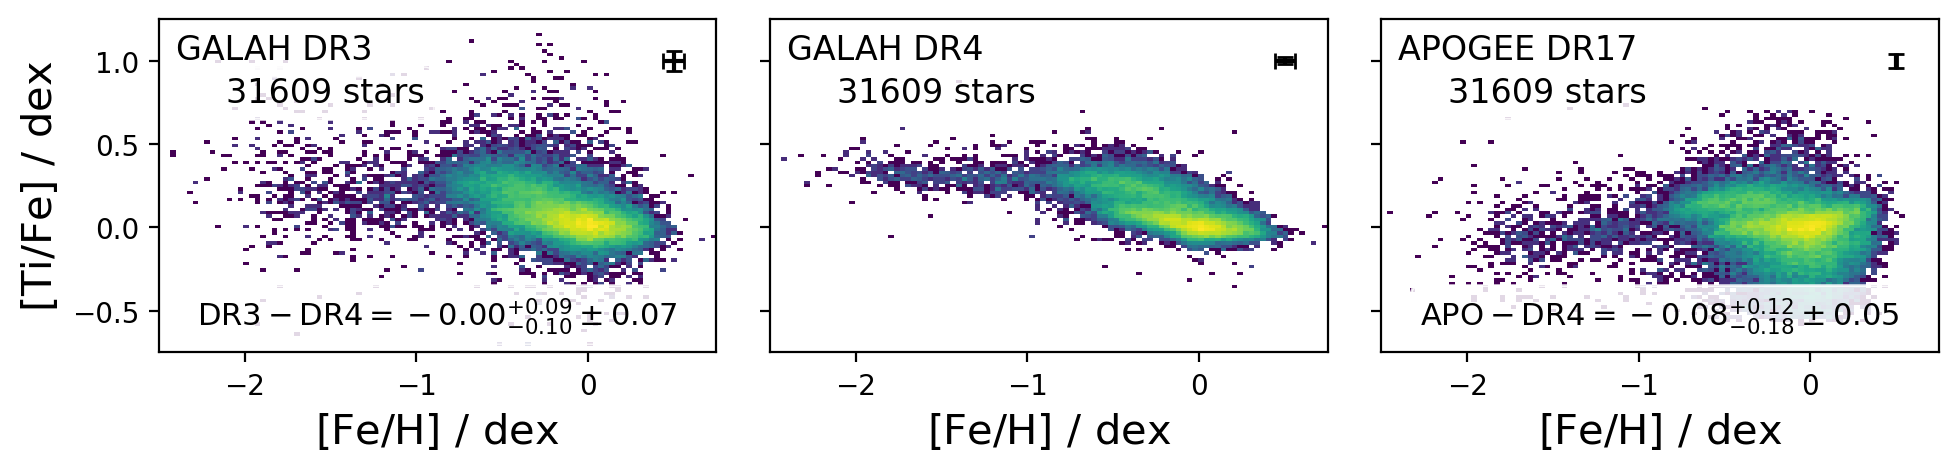
\includegraphics[width=0.87\textwidth]{figures/comparison_dr4_dr3_apo17_Ti_fe.png}
 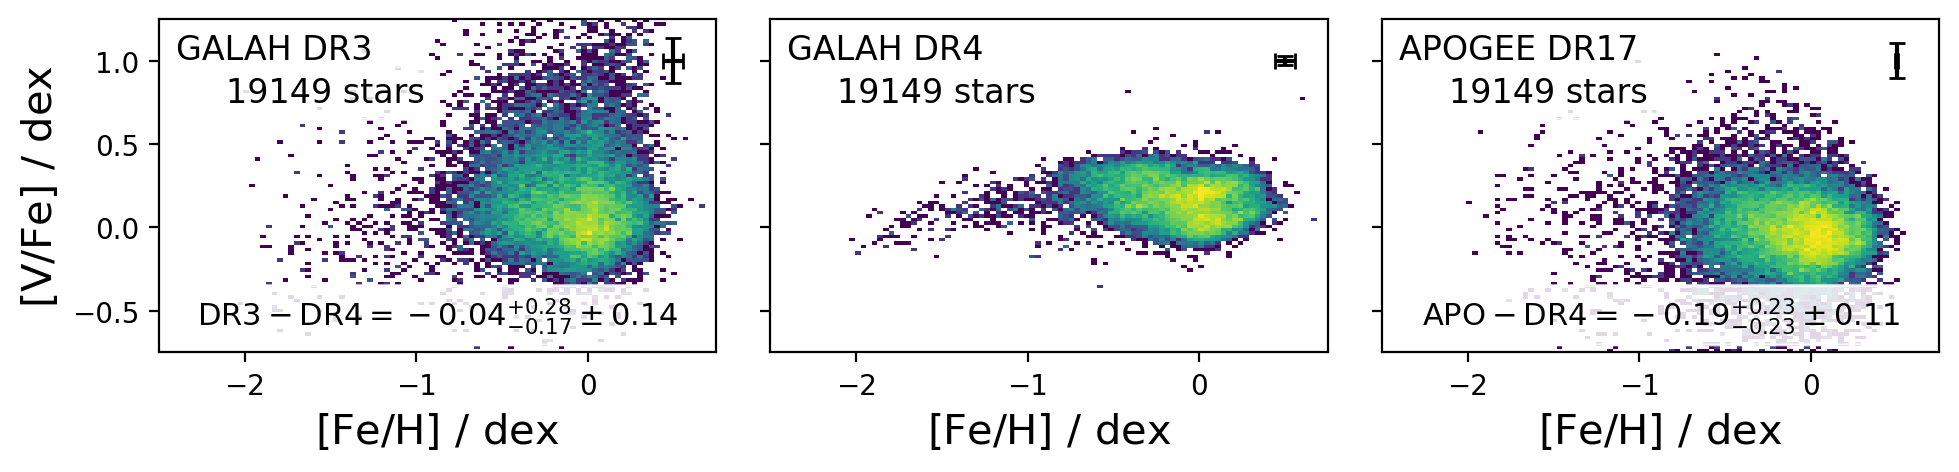
\includegraphics[width=0.87\textwidth]{figures/comparison_dr4_dr3_apo17_V_fe.png}
 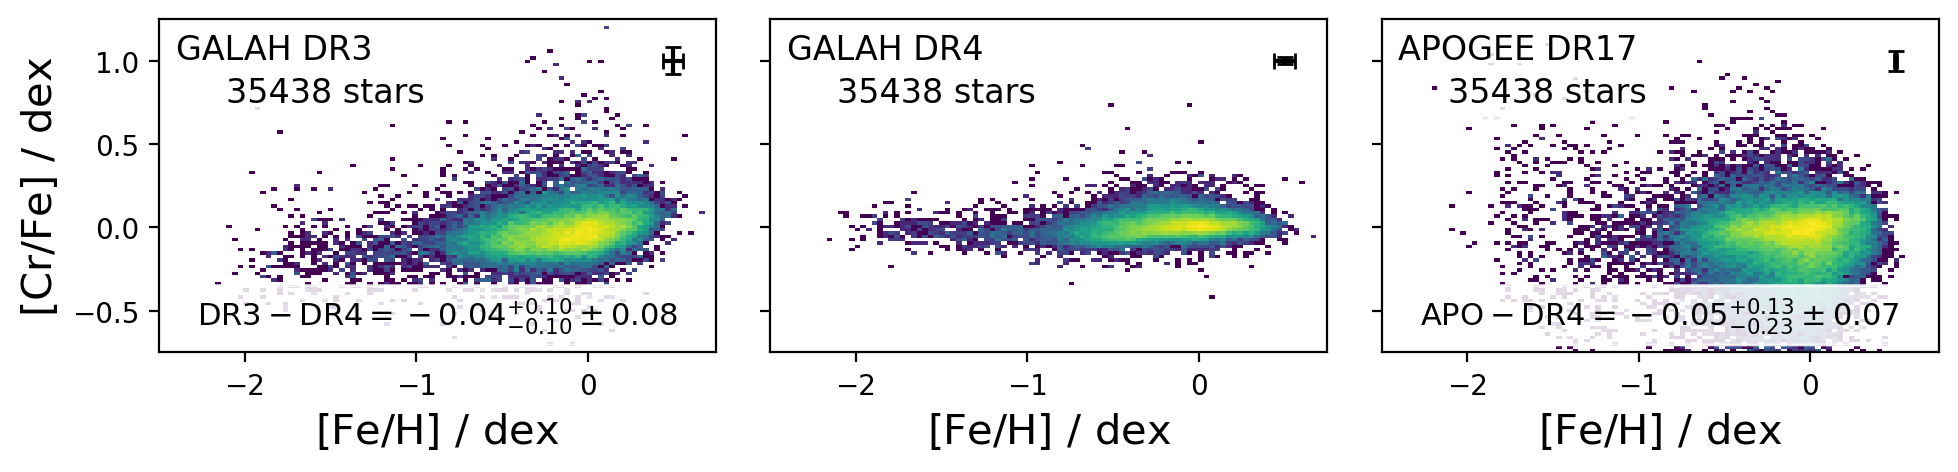
\includegraphics[width=0.87\textwidth]{figures/comparison_dr4_dr3_apo17_Cr_fe.png}
 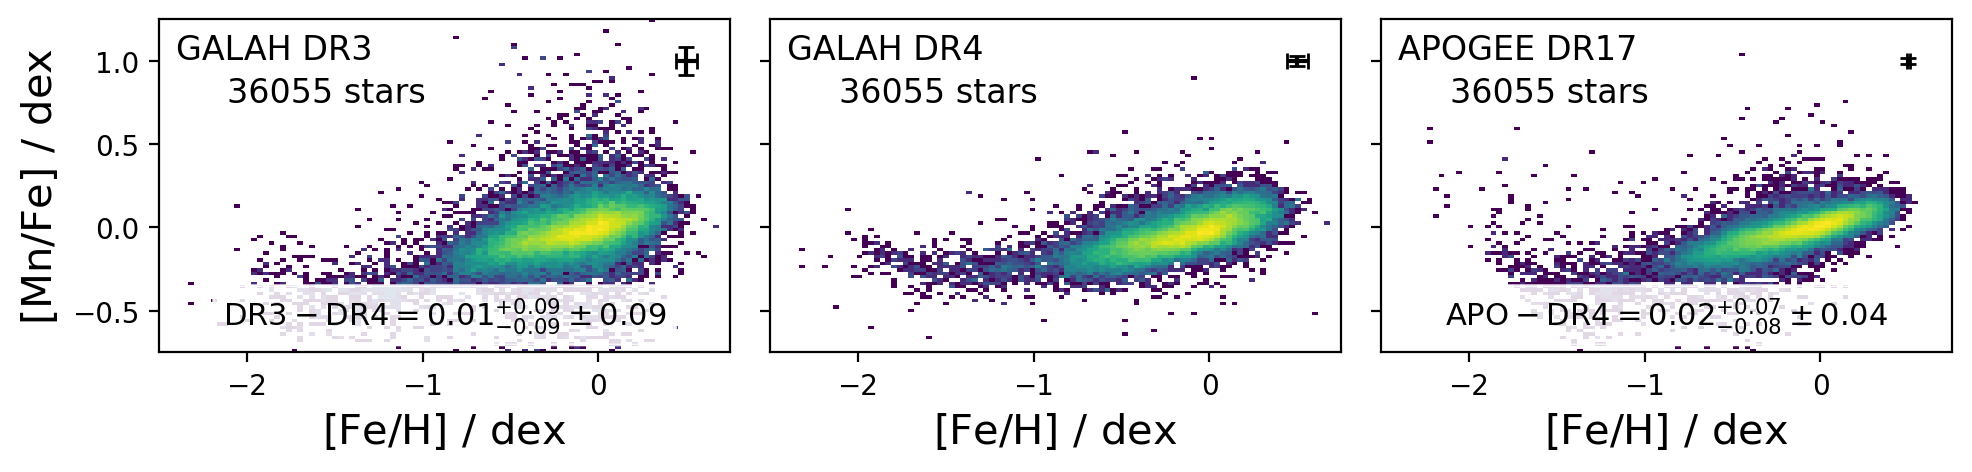
\includegraphics[width=0.87\textwidth]{figures/comparison_dr4_dr3_apo17_Mn_fe.png}
 \includegraphics[width=0.87\textwidth]{figures/comparison_dr4_dr3_apo17_Co_fe.png}
 \includegraphics[width=0.87\textwidth]{figures/comparison_dr4_dr3_apo17_Ce_fe.png}
 \caption{\textbf{Continuation of Fig.~\ref{fig:comparison_dr3_dr4_apo17_rest} for Ti, V, Cr, Mn, Co, and Ce}.}
 \label{fig:comparison_dr3_dr4_apo17_rest2}
\end{figure*}


% \begin{landscape}
\begin{figure*}
\includegraphics[width=\textwidth]{figures/galah_dr4_gcs_teff_logg.png}
\caption{
\textbf{Collage of globular clusters in the \Teff-\logg space, coloured by stellar metallicity \feh.} There are only minor trends between \feh and \Teff, even for the horizontal branch stars in NGC 288, NGC 6656 (M22), and NGC 6121 (M4). NGC 5139 ($\upomega$Cen) shows a significant range in \feh. RMS scatter and median metallicity uncertainties for each cluster are given in the lower right of each panel.}
\label{fig:galah_dr4_gcs_teff_logg}
\end{figure*}
% \end{landscape}

Although multiple of the observed globular clusters are expected to show an abundance spread, including for iron, we show a collage of globular clusters with ascending iron abundance in Fig.~\ref{fig:galah_dr4_gcs_teff_logg}, with each panel indicating the median iron abundance per cluster as well as the spread (scatter) of the iron abundance distribution and the average measurement uncertainty. A more comprehensive analysis of the globular clusters will be presented in upcoming work (McKenzie et al., in preparation).

\subsection{Distribution of flagged stars}

Fig.~\ref{fig:flag_sp_overview_allstar}

\begin{figure*}[ht]
 \centering
 \includegraphics[width=\textwidth]{figures/flag_sp_overview_allstar.png}
 \caption{\textbf{Parameter overview of stars with raised major quality flag \texttt{flag\_sp} for \texttt{allstar}.}
 \textbf{Each panel} shows the logarithmic density distribution of stars in the \Teff and \logg plane with blue colormaps. A PARSEC isochrone with $\mathrm{[M/H]}=0$ and $\tau = 4.5\,\mathrm{Gyr}$ is overplotted in orange and the same mass binary main sequence (shifted from the single star one by $\Delta \log g = -0.3\,\mathrm{dex}$) is shown in red. Panel heads denote the bit mask and its description as well as how many times the flag was raised. We neglect distributions with no flag (0), for flags which have not been raised (8,9,11), and for which no results were available (15).} \label{fig:flag_sp_overview_allstar}
\end{figure*}

\end{document}
